\Huge{ \tb{Brouillion}}\normalsize

\subsection{Generic formulations}

Now that we reached a clear understanding of the averaged models, we introduce the Hybrid model for dispersed two phase flows. 

As it has been shown in earlier studies \citep{jackson2000dynamics,chu2016flux} it is more physical to express the non-convective flux appearing in \ref{eq:avg_dt_chi_f} with the volume fraction outside the divergence operator. 
These considerations finally leads us to the general form of the continuous phase equation : 
\begin{equation}
    \pddt (\phi_1 f_1)
    + \div (\phi_1 f_1\textbf{u}_1
    + \phi_1 \bm{\Phi}^\text{Re}_1)
    = 
    \phi_1(s_1  +\div \mathbf{\Phi}_1)
    - n_p \textbf{F}_p
    \label{eq:hybrid_avg_dt_chif}
\end{equation}
Where we introduced the following definition, 
\begin{align*}
    \textbf{F}_\alpha 
    &= 
    \int_{\Sigma_\alpha}
    \left(
        \mathbf{\Phi}_1^0 
        - \mathbf{\Phi}_1
    \right)  
    \cdot \textbf{n}_2d\Sigma
    + 
    \int_{\Sigma_\alpha}f_1^0
    \left(
        \textbf{u}_I^0
        - \textbf{u}_1^0
    \right)
    \cdot \textbf{n}_2d\Sigma,\\
    \textbf{M}_\alpha 
    &= \int_{\Sigma_\alpha} \textbf{r}
        \left(\mathbf{\Phi}_1^0- \mathbf{\Phi}_1\right)\cdot \textbf{n}_2d\Sigma
        + \int_{\Sigma_\alpha} \textbf{r}f_1^0
        \left(
            \textbf{u}_I^0
            - \textbf{u}_1^0
        \right)
    \cdot \textbf{n}_2d\Sigma\\
    \bm{\Phi}^\text{Re}_1
    &= \oneavg{f_1' \textbf{u}_1'}  - \textbf{M}_p n_p
\end{align*}
where we neglected the second order moment or higher moments. 

Regarding the dispersed phase, we consider the zeroth and first moment equation (\ref{eq:avg_dt_dq_alpha_tot} and \ref{eq:avg_dt_dQ_alpha_tot}) as  a part of the hybrid model.
Under this form the couplings terms in \ref{eq:hybrid_avg_dt_chif} do not correspond to the ones appearing in both, \ref{eq:avg_dt_dq_alpha_tot} and \ref{eq:avg_dt_dQ_alpha_tot} which is essential for ensuring a consistent model. 
To fix this problem we reformulated both exchange terms following \citet{zhang1997momentum} such that it correspond to $\mathbf{F}_\alpha$ and $\textbf{M}_\alpha$. 
Then we may rewrite the momentum and moment of momentum equations (\ref{eq:avg_dt_dq_alpha_tot} and \ref{eq:avg_dt_dQ_alpha_tot}) as : 
\begin{multline}
    \pddt \left(n_p q_p^\text{tot}\right)
    + \div \left(n_p\textbf{u}_p
    q_p^\text{tot} + 
    \textbf{q}_p^\text{Re}
    \right)
    = 
    n_p v_p  \div \mathbf{\Phi}_1 
    + n_p \textbf{F}_p,
    + \pnavg{\int_{\Omega_\alpha} s_2 d\Omega}
    + \pnavg{\int_{\Sigma_\alpha} s_I d\Sigma}
    \label{eq:hybrid_avg_dt_q_alpha}
\end{multline}
\begin{multline}
    \pddt \left(n_p \mathcal{Q}_p^\text{tot}\right)
    + \div \left(
        n_p \textbf{u}_p \mathcal{Q}_p^\text{tot}
    + \mathcal{Q}_p^\text{Re}
    \right)
    =
    n_p v_p \mathbf{\Phi}_1 
    + n_p \textbf{M}_p\\
    \pnavg{\int_{\Omega_\alpha} \left(
        \textbf{r} s_2^0         
        + f_2^0  \textbf{w}_2^0 
        - \mathbf{\Phi}_2^0
        \right) d\Omega}
        + \pnavg{\int_{\Sigma_\alpha} \left(
        \textbf{r}s_I^0
        + f_I^0 \textbf{w}_I^0
        - \mathbf{\Phi}_{I||}^0
    \right) d\Sigma},
    \label{eq:hybrid_avg_dt_Q_alpha}
\end{multline}
respectively. 
Where  we introduced the following notation
\begin{align*}
    \textbf{q}_p^\text{Re}
    &= 
    \pnavg{\textbf{u}_\alpha'(q_\alpha'+q_{I_\alpha}')} \\
    \mathcal{Q}_p^\text{Re}
    &= 
    + \pnavg{\textbf{u}_\alpha'(\mathcal{Q}_\alpha'+\mathcal{Q}_{I_\alpha}')'}
\end{align*}

Then, \ref{eq:hybrid_avg_dt_chif}, \ref{eq:hybrid_avg_dt_q_alpha} and \ref{eq:hybrid_avg_dt_Q_alpha}, are the most general form of a first-order accurate hybrid model for arbitrary particle. 
Lastly, it is worth noting that by incorporating more terms in the expansion of \ref{eq:avg_dt_chi_f} and higher order moments equations, one can reach an arbitrary order of accuracy, as stated by \citet{zhang1997momentum}. 


\subsubsection{The Reynolds stress due to wake}
The fluctuation term $\avg{\chi_1 \textbf{u}_1'\textbf{u}_1'}$ can be reformulated. 
It must have an isotropic component and a component slightly higher in teh direction of the relative velocity.  
First of all the trace can be written down with, 
\begin{equation*}
    k_1=
    \frac{1}{2}\textbf{I}:\oneavg{\textbf{u}_1'\textbf{u}_1'}
\end{equation*}
The deviatoric part is then, 
\begin{equation*}
    (\oneavg{\textbf{u}_1'\textbf{u}_1'})^\text{dev}=
    \oneavg{\textbf{u}_1'\textbf{u}_1'}
    - \frac{2}{3}k_1\textbf{I}
\end{equation*}
If we assume the form, 
\begin{equation*}
    \oneavg{\textbf{u}_1'\textbf{u}_1'}
    = 
    \textbf{U}
    \textbf{U}
    k^{||}_1
    + 
    \left[
        \textbf{I} (\textbf{U}\cdot \textbf{U})
    -
    \textbf{U}
    \textbf{U}
    \right]
    k^{\bot}_1
    = 
    \textbf{U}
    \textbf{U}
    (k^{||}_1 - k^{\bot}_1)
    + \textbf{I} (\textbf{U}\cdot\textbf{U}) k^\bot_1
\end{equation*}
where $\textbf{U} = (\textbf{u}_p - \textbf{u}_f)$. 
Since the velocity fluctuation is higher in the flow direction $k^\bot_1 < k_1 < k^{||}_1$. 
The last expression is the one usually used. 
However, we would like to see appear $k_1$ in this expression since we solve an equation for $k_1$.  
The ultimate goal is to factor out $k_1$ from the above expression thus note that :
\begin{align*}
    k_1 =
    \frac{1}{2} \oneavg{\textbf{u}_1'\textbf{u}_1'} : \textbf{I}
    &= 
    \frac{1}{2} \textbf{U}
    \textbf{U}
    (k^{||}_1 - k^{\bot}_1) : \textbf{I}
    + \frac{1}{2} \textbf{I} (\textbf{U}\cdot\textbf{U}) k^\bot_{||} : \textbf{I}\\
    &= 
    \frac{1}{2} 
    \textbf{U}\cdot 
    \textbf{U}
    (k^{||}_1 - k^{\bot}_1)
    + \frac{3}{2}  (\textbf{U}\cdot\textbf{U}) k^\bot_1 \\
    &= 
    \frac{1}{2} 
    (\textbf{U}\cdot 
    \textbf{U})[
        k^{||}_1 
        + 2 k^\bot_1
    ]\\
    &= 
    (\textbf{U}\cdot 
    \textbf{U})[
        \frac{1}{2}k^{||}_1 
        + k^\bot_1
    ]
\end{align*}
Let's add and subtract $\frac{1}{2}\textbf{I}(\textbf{U}\cdot\textbf{U})(k^{||}_1)$ to the previous expression of the Reynolds stress, 
\begin{align*}
    \oneavg{\textbf{u}_1'\textbf{u}_1'}
    &= 
    \textbf{U}
    \textbf{U}
    (k^{||}_1 - k^{\bot}_1)
    + \textbf{I} 
    (\textbf{U}\cdot\textbf{U}) k^\bot_1
    + \frac{1}{2}\textbf{I} 
    (\textbf{U}\cdot\textbf{U}) (k^{||}_1)
    - \frac{1}{2}\textbf{I} 
    (\textbf{U}\cdot\textbf{U}) (k^{||}_1)\\
    &= 
    \textbf{U}
    \textbf{U}
    (k^{||}_1 - k^{\bot}_1)
    - \frac{1}{2}\textbf{I} 
    (\textbf{U}\cdot\textbf{U}) k^{||}_1
    + \textbf{I} 
    (\textbf{U}\cdot\textbf{U}) k^*_1
    \\
\end{align*}
where $ k^*_1 = k_1 /(\textbf{U}\cdot \textbf{U})$ is the dimensionless granular temperature.  

To introduce a simpler notation we pose $k^{||}_1 = (C_1 +1/3) 2k_1^*$ and $k^{\bot}_1 = (C_2+1/3) 2k_1^*$ so that in the isotope scenario,  when $k^{||}_1 = \frac{2}{3} k^*_1$ or $k^{||}_1 =\frac{2}{3} k^*_1$ the constant $C_1$ and $C_2$ equal zero. 
\begin{align*}
    \oneavg{\textbf{u}_1'\textbf{u}_1'}
    &= 
    \textbf{U}
    \textbf{U}
    ((C_1 +1/3)2k_1^* -( C_2+1/3) 2 k_1^*)
    - \frac{1}{2}\textbf{I} 
    (\textbf{U}\cdot\textbf{U})  (C_1+1/3) 2k_1^*
    + \textbf{I} 
    (\textbf{U}\cdot\textbf{U}) k^*_1\\
    &= k^*_1 \left[
        \textbf{U}
        \textbf{U}
        (C_1  - C_2 )
        + \textbf{I} 
        (\textbf{U}\cdot\textbf{U})  (C_1+2/3) 
    \right]
\end{align*}
Note that when, $C_1=C_2= 0$ we recover $\oneavg{\textbf{u}_1'\textbf{u}_1'}=\frac{2}{3} \textbf{I}(\textbf{U}\cdot \textbf{U}) k^*_1$

\section{The ultimate model ?}
The main idea is to let the internal viscous term of particles : $\lambda \phi_2 \bm{\tau}_2$ within the divergence of the momentum equation to recover the proper Stresslet term, i.e $\mathscr{S}_p = n_p(\textbf{r} \bm{\sigma}_1^0 \cdot \textbf{n})_p^\Sigma -n_p(\textbf{r} \cdot \bm{\sigma}_1^0 \cdot \textbf{n})_p^\Sigma \textbf{I} - \lambda \phi_2 \bm{\tau}_2$. 
The trace of the stress let might be removed by the use of the averaged pressure $p_1$ present in the models below. 
How about the viscosity ratio part ? Well it can be show that, 
\begin{align*}
    n_p (\textbf{r} \bm{\sigma}_1'\cdot \textbf{n}_1)_p^\Sigma
    = 
    n_p (\textbf{r} \bm{\sigma}_1^0\cdot \textbf{n}_1)_p^\Sigma
    - n_p v_p \bm{\sigma}_1 
\end{align*}
From the formulas, 
\begin{align*}
    \bm{\sigma}_1 \phi_1
    &=- \phi_1 p_1 \textbf{I}
    + \mu_1 \textbf{e}
    - \lambda \phi_2 \bm{\tau}_2\\
    \bm{\sigma}_1 n_p v_p 
    &=- n_p v_p p_1 \textbf{I}
    + \frac{n_p v_p}{\phi_1}\mu_1 \textbf{e}
    - \lambda \frac{n_pv_p\phi_2}{\phi_1} \bm{\tau}_2
\end{align*}
we see that we hardly recover the real stresslet, because under this form the term related to the particle shear is lumped into the divergence at the other side of the equations. 
Therefore, the BEST model is the one were we throw $-p_1$ and $\textbf{q}_1$ on the Others side of the  equaiton. 
Note that the trace of $n_p(\textbf{r} \cdot (\bm{\sigma}_1^0 - p_1) \cdot \textbf{n})_p^\Sigma \textbf{I}$ is surely null since no pressure force form the normal viscous force is possible. 

In a shearing problem this might be not the best option because the mean shear isn't subtracted to the drag and first moment. 

\subsection*{Fluid phase}

Using the generic formulation \ref{eq:hybrid_avg_dt_chif} and the local expression of the mass, momentum and total energy expression, i.e. : \ref{eq:dt_rho},\ref{eq:dt_rhou_k} and \ref{eq:dt_rhoE_k} we easily find the averaged form of these equations as, 
\begin{align}
    \label{eq:dt_&vg_rho}
    \pddt (\phi_1 \rho_1)  
    + \div (
        \phi_1 \rho_1\textbf{u}_1
    )
    &= 
    0\\
    \label{eq:dt_&vg_rhou_1}
    \pddt (\phi_1 \rho_1\textbf{u}_1)  
    + \div (
        \phi_1 \rho_1\textbf{u}_1\textbf{u}_1
        + \bm{\sigma}_1^\text{eq}
    )
    &= 
    \phi_1 (\rho_1 \textbf{g} 
    - \grad p_1 ) 
    -  \avg{\delta_I \bm{\sigma}_1' \cdot \textbf{n}_2}\\
    \label{eq:dt_&vg_rhoE_1}
    \pddt (\phi_1\rho_1E_1)  
    + \div (
        \phi_1\rho_1E_1\textbf{u}_1
        + \bm{q}_1^\text{eq}
        + \textbf{u}_1 \cdot \bm{\sigma}_1^\text{eq}
        % - \textbf{u}_1^0 \cdot \bm{\sigma}_1^0 
        % + \textbf{q}_1^0
        )
    &= 
    \phi_1 [\rho_1\textbf{u}_1 \cdot \textbf{g} 
    - \div(\textbf{u}_1p_1 + \textbf{q}_1)]
    - \textbf{u}_1 \cdot\avg{\delta_I \bm{\sigma}_1'\cdot \textbf{n}_2}\nonumber\\
    &- \avg{\delta_I (\textbf{u}_1' \cdot \bm{\sigma}_1^0 )\cdot \textbf{n}_2}
    + \avg{\delta_I\textbf{q}_1'\cdot \textbf{n}_2}
\end{align} 
\begin{align*}
    &\bm{\sigma}_1^\text{eq}
    = \phi_1\rho_1\kavg{\textbf{u}_1'\textbf{u}_1'}
    - \bm{\tau}_1 \phi_1
    &\textbf{q}_1^\text{eq}
    =\textbf{q}_1^\text{e} +\textbf{q}_1^\text{k}  \\
    &\textbf{q}_1^\text{e}
    = \phi_1\rho_1 \kavg{\textbf{u}_1' e_1'} 
    &\textbf{q}_1^\text{k}
    = \phi_1\rho_1 \kavg{\textbf{u}_1' k_1} 
    - \phi_1\kavg{\textbf{u}_1' \cdot \bm{\sigma}_1^0}
\end{align*}
Applying the energy decomposition, 
\begin{align}
    \pddt (\phi_1 \rho_1u_1^2/2)  
    + \div (
        \phi_1 \rho_1\textbf{u}_1u_1^2/2
        + \textbf{u}_1 \cdot \bm{\sigma}_1^\text{eq}
    )
    &= 
    + \bm{\sigma}_1^\text{eq} : \grad \textbf{u}_1
    + \phi_1  \textbf{u}_1\cdot(\rho_1 \textbf{g} - \grad p_1) 
    -  \textbf{u}_1\cdot \avg{\delta_I \bm{\sigma}_1' \cdot \textbf{n}_2}\\
    \pddt (\phi_1\rho_1k_1)  
    + \div (
        \phi_1\rho_1k_1\textbf{u}_1
        + \textbf{q}_1^\text{k} 
        )
    &= 
    - \textbf{d}_1
    - (\phi_1 p_1 + \bm{\sigma}_1^\text{eq} ): \grad \textbf{u}_1
    - \avg{\delta_I \textbf{u}_1' \cdot \bm{\sigma}_1^0 \cdot \textbf{n}_2}\\
    \pddt (\phi_1\rho_1e_1)  
    + \div (
        \phi_1 \rho_1e_1\textbf{u}_1
        +
        \textbf{q}_1^\text{e} 
        )
    &= 
    \textbf{d}_1
    - \phi_1 \div \textbf{q}_1
    + \avg{\delta_I \textbf{q}_1' \cdot \textbf{n}_2} 
\end{align}
The interfacial terms in the momentum equation can be reformulated as,
\begin{align*}
    \avg{\delta_I \bm{\sigma}_1' \cdot \textbf{n}_2}
    = n_p \textbf{f}_\text{p} - \div (n_p \mathcal{F}_p)\\
    \avg{\delta_I (\textbf{u}_1' \cdot \bm{\sigma}_1^0)\cdot \textbf{n}_2}
    = n_p \textbf{c}_\text{p} - \div (n_p\mathcal{C}_p)\\
    \avg{\delta_I \textbf{q}_1 \cdot \textbf{n}_2}
    = n_p \textbf{q}_\text{p} - \div (n_p \mathcal{Q}_p)
\end{align*}
The new equations are then, 
\begin{align}
    \pddt (\phi_1 \rho_1)  
    + \div (
        \phi_1 \rho_1\textbf{u}_1
    )
    &= 
    0\\
    \pddt (\phi_1 \rho_1\textbf{u}_1)  
    + \div (
        \phi_1 \rho_1\textbf{u}_1\textbf{u}_1
        + \bm{\sigma}_1^\text{eq}
    )
    &= 
    \phi_1 (\rho_1 \textbf{g} 
    - \grad p_1 ) 
    -  n_p \textbf{f}_p\\
    \pddt (\phi_1\rho_1E_1)  
    + \div (
        \phi_1\rho_1E_1\textbf{u}_1
        + \bm{q}_1^\text{eq}
        + \textbf{u}_1 \cdot \bm{\sigma}_1^\text{eq}
        )
    &= 
    -n_p \mathcal{F}_p :\grad \textbf{u}_1
    +\phi_1 [\rho_1\textbf{u}_1 \cdot \textbf{g} 
    - \div(\textbf{u}_1p_1 + \textbf{q}_1)]\nonumber\\
    &- n_p \textbf{u}_1 \cdot \textbf{f}_p
    - n_p \textbf{c}_p
    + n_p \textbf{q}_p
\end{align} 
\begin{align*}
    &\bm{\sigma}_1^\text{eq}
    = \phi_1\rho_1\kavg{\textbf{u}_1'\textbf{u}_1'}
    - \bm{\tau}_1 \phi_1
    - n_p \mathcal{F}_p
    &\textbf{q}_1^\text{eq}
    =\textbf{q}_1^\text{e} +\textbf{q}_1^\text{k} \\
    &\textbf{q}_1^\text{e}
    = \phi_1\rho_1 \kavg{\textbf{u}_1' e_1'} + n_p \mathcal{Q}_p
    &\textbf{q}_1^\text{k}
    = \phi_1\rho_1 \kavg{\textbf{u}_1' k_1} 
    - \phi_1\kavg{\textbf{u}_1' \cdot \bm{\sigma}_1^0}
    - n_p \mathcal{C}_p 
\end{align*}
The energies equations can be written : 
\begin{align}
    \pddt (\phi_1 \rho_1u_1^2/2)  
    + \div (
        \phi_1 \rho_1\textbf{u}_1u_1^2/2
        + \textbf{u}_1 \cdot \bm{\sigma}_1^\text{eq}
    )
    &= 
    + \bm{\sigma}_1^\text{eq} : \grad \textbf{u}_1
    + \phi_1  \textbf{u}_1\cdot(\rho_1 \textbf{g} - \grad p_1) 
    - n_p \textbf{u}_1\cdot \textbf{f}_p\\
    \pddt (\phi_1\rho_1k_1)  
    + \div (
        \phi_1\rho_1k_1\textbf{u}_1
        + \textbf{q}_1^\text{k} 
        )
    &= 
    - \textbf{d}_1
    + \phi_1(\bm{\sigma}_1 - \rho_1 \oneavg{\textbf{u}_1'\textbf{u}_1'} ): \grad \textbf{u}_1
    - n_p \textbf{c}_p\\
    \pddt (\phi_1\rho_1e_1)  
    + \div (
        \phi_1 \rho_1e_1\textbf{u}_1
        +
        \textbf{q}_1^\text{e} 
        )
    &= 
    \textbf{d}_1
    - \phi_1 \div \textbf{q}_1
    + n_p \textbf{q}_p
\end{align}
It is interesting to note that the first moment of hydrodynamic forces appear under inside the macroscopic sink term. 
Inside the kinetic energy only the higher moment of the exchange terms appear. 
And so on for the internal energy. 


\subsection*{Particules phase}
Regarding the dispersed phase we have  if we assume a certain error we obtain :
\begin{align*}
    \pddt \left(n_p m_p\right)
    + \div \left(n_pm_p\textbf{u}_p
    \right)
    = 
    0\\
    \pddt \left(n_p m_p \textbf{u}_p\right)
    + \div \left(n_p
    m_p \textbf{u}_p \textbf{u}_p 
    + \bm{\sigma}_p^\text{eq}
    \right)
    = 
    n_p v_p (\rho_2 \textbf{g}
    - \grad p_1)
    + n_p (\bm{\sigma}_1' \cdot \textbf{n}_2)_p^\Sigma,\\
    \pddt(m_p n_pE_p^\text{tot})
    + \div(m_pn_p E_p^\text{tot} \textbf{u}_p 
    + \textbf{q}_p^\text{eq} 
    + \textbf{u}_p \cdot \bm{\sigma}_p^\text{eq})
    =  n_p v_p [\rho_2 \textbf{u}_p\cdot  \textbf{g}
    - \div (\textbf{u}_1 p_1 + \textbf{q}_1)]\\
    % +  n_p ( \textbf{u}'_1 \cdot \bm{\sigma}_1^0 \cdot \textbf{n}_2)_p^\Sigma
    -  n_p (\textbf{q}_1' \cdot \textbf{n}_2)_p^\Sigma
    +  n_p (\textbf{u}_1 \cdot \bm{\sigma}_1' \cdot \textbf{n}_2)_p^\Sigma
    +  n_p (\textbf{u}_1' \cdot \bm{\sigma}_1^0\cdot \textbf{n}_2)_p^\Sigma
\end{align*}
\begin{align*}
    &\bm{\sigma}_p^\text{eq}
    = m_p\pnavg{\textbf{u}_\alpha'\textbf{u}_\alpha'}
    &\textbf{q}_p^\text{eq}
    =\textbf{q}_p^\text{e} 
    +\textbf{q}_p^\text{k}  
    +\textbf{q}_p^\text{w}  
    \\
    &\textbf{q}_1^\text{e}
    = m_p \pnavg{\textbf{u}_\alpha' e_\alpha'} 
    &\textbf{q}_p^\text{k}
    = m_p \pnavg{\textbf{u}_\alpha' k_\alpha} 
    \\
    &\textbf{q}_p^\text{w}
    = 
    + \pnavg{\textbf{u}_\alpha'(\rho_2 (w^0_2)^2/2 )'_\Omega}
    + \gamma \pnavg{\textbf{u}_\alpha' s_\alpha'}
\end{align*}
Following the energy decomposition : 
\begin{align*}
    \avg{\delta_I (\bm{\sigma}_1^0 ) \textbf{n}_2} - p_1 \grad \phi_1
    = 
    % \avg{\delta_I (\bm{\sigma}_1^0 + p_1)\cdot \textbf{n}_2}
    % = 
    \avg{\delta_I \bm{\sigma}_1'\cdot \textbf{n}_2}
    \\
    \avg{\delta_I (\textbf{u}_1^0 \cdot\bm{\sigma}_1^0 )} - \textbf{u}_1p_1\cdot \grad \phi_1
    % = \avg{\delta_I (\textbf{u}_1 \cdot \bm{\sigma}_1' + \textbf{u}_1' \cdot \bm{\sigma}_1^0 )\cdot \textbf{n}_2}
    = \textbf{u}_1 \cdot \avg{\delta_I \bm{\sigma}_1'\cdot \textbf{n}_2}
    + \avg{\delta_I (\textbf{u}_1' \cdot \bm{\sigma}_1^0 )\cdot \textbf{n}_2}
\end{align*}

The energy decomposition :
\begin{align*}
    E_1 = e_1 + k_1 + u_k^2/2
\end{align*}
\begin{equation*}
    n_p m_p E_p(t) 
    = m_p n_p e_p 
    + \pnavg{\int_{\Omega_\alpha(t)} \rho_2  (w_2^0)^2/2 d\Omega}
    + m_p n_p k_p
    + m_p n_p (u_p)^2/2
    + n_p s_p \gamma
    % + \textbf{u}_\alpha \cdot \int_{\Omega_\alpha(t)} \rho_2  \textbf{w}_2^0 d\Omega
\end{equation*}


we obtain the following system of equaiton 
\begin{align*}
    &\pddt \left(n_p m_p u_p^2/ 2\right)
    + \div \left(n_p
    m_p u_p^2/ 2 \textbf{u}_p 
    + \textbf{u}_p \cdot \bm{\sigma}_p^\text{eq}
    \right)
    = 
     \bm{\sigma}_p^\text{eq}  :\grad \textbf{u}_p
    +  n_p v_p \textbf{u}_p \cdot 
    (\rho_2 \textbf{g} - \grad p_1)
    + n_p \textbf{u}_p \cdot (\bm{\sigma}_1' \cdot \textbf{n}_2)^\Sigma_p,\\
    &\pddt \left(n_p m_p (u_\alpha^2)_p/ 2\right)
    + \div \left(n_p
    m_p (u_\alpha^2)_p/ 2 \textbf{u}_p 
    + \textbf{q}^k_p
    + \textbf{u}_p \cdot \bm{\sigma}_p^\text{eq}
    \right)
    = 
    n_p v_p \textbf{u}_p \cdot
    (\rho_2 \textbf{g} - \grad p_1)
    + n_p\textbf{u}_p\cdot (\bm{\sigma}_1' \cdot \textbf{n}_2)^\Sigma_p\\
    &+n_p(\textbf{u}_\alpha'\cdot(\bm{\sigma}_1^0 \cdot \textbf{n}_2)^\Sigma)_p
    \\
    &\pddt \left(n_p (\rho_2 w^2 )_p^\Omega+\gamma s_p n_p\right)
    + \div 
    (n_p (\rho_2 w^2 )_p^\Omega+\gamma s_p n_p
    \textbf{u}_p 
    +  \textbf{q}_p^\text{w}
    )
    = 
    - n_p (\bm{\sigma}_2^0 : \grad\textbf{u}_2^0)^\Omega_p
    % + n_p (\textbf{u}_1^0 \cdot \bm{\sigma}_1^0 \cdot  \textbf{n}_2)^\Sigma_p
    + n_p (\textbf{w}_1^0 \cdot \bm{\sigma}_1^0 \cdot  \textbf{n}_2)^\Sigma_p\\
    &\pddt \left(n_p m_p e_p\right)
    + \div \left(n_p
    m_p e_p \textbf{u}_p 
    +  \textbf{q}_p^\text{e}
    \right)
    = 
    + n_p (\bm{\sigma}_2^0 : \grad\textbf{u}_2^0)^\Omega_p
    - n_p v_p \div \textbf{q}_1
    - n_p (\textbf{q}_1'\cdot \textbf{n}_2)^\Sigma_p\\
\end{align*}


From the two first equations it is evident that the granular temperature equation is, 
\begin{multline*}
    \pddt(m_p n_pk_p)
    + \div(m_pn_p k_p \textbf{u}_p 
    + \textbf{q}_p^\text{k})
    = 
     - \bm{\sigma}_p^\text{eq}  :\grad \textbf{u}_p
     + n_p (\textbf{u}_\alpha' \cdot (\bm{\sigma}_1^0 \cdot  \textbf{n}_2)^\Sigma)_p
    \\
\end{multline*}

In the total NRJ equations can re express the terms 
\begin{multline*}
    n_p (\textbf{u}_1 \cdot \bm{\sigma}_1' \cdot  \textbf{n}_2)^\Sigma_p
    = 
    n_p (\textbf{u}_1(\textbf{x}_\alpha) \cdot \bm{\sigma}_1' \cdot  \textbf{n}_2)^\Sigma_p
    + n_p (\textbf{r}\grad\textbf{u}_1(\textbf{x}_\alpha) \cdot \bm{\sigma}_1' \cdot  \textbf{n}_2)^\Sigma_p
    =n_p \textbf{u}_1 \cdot \textbf{f}_p
    + n_p \mathcal{F}_p :\grad \textbf{u}_1
\end{multline*}
Besides note that without mass transfert and with incompressible fluid the internal fluctuation source term yields,
\begin{multline*}
    (\textbf{w}_1^0 \cdot \bm{\sigma}_1^0 \cdot  \textbf{n}_2)^\Sigma_p
    =   
    (\textbf{w}_1^0 \cdot \bm{\sigma}_1' \cdot  \textbf{n}_2)^\Sigma_p
    =   
    (\textbf{u}_1^0 \cdot \bm{\sigma}_1^0 \cdot  \textbf{n}_2)^\Sigma_p
    - \textbf{u}_p \cdot (\bm{\sigma}_1^0 \cdot  \textbf{n}_2)^\Sigma_p
    - (\textbf{u}_\alpha' \cdot \bm{\sigma}_1^0 \cdot  \textbf{n}_2)^\Sigma_p\\
    =   
    (\textbf{u}_1 \cdot \bm{\sigma}_1^0 \cdot  \textbf{n}_2)^\Sigma_p
    + (\textbf{u}_1' \cdot \bm{\sigma}_1^0 \cdot  \textbf{n}_2)^\Sigma_p
    - \textbf{u}_p \cdot (\bm{\sigma}_1^0 \cdot  \textbf{n}_2)^\Sigma_p
    - (\textbf{u}_\alpha' \cdot \bm{\sigma}_1^0 \cdot  \textbf{n}_2)^\Sigma_p\\
    =   
    (\textbf{r}\bm{\sigma}_1^0 \cdot  \textbf{n}_2)^\Sigma_p : \grad \textbf{u}_1+
    (\textbf{u}_1 - \textbf{u}_p) \cdot (\bm{\sigma}_1^0 \cdot  \textbf{n}_2)^\Sigma_p
    + (\textbf{u}_1' \cdot \bm{\sigma}_1^0 \cdot  \textbf{n}_2)^\Sigma_p
    - (\textbf{u}_\alpha' \cdot \bm{\sigma}_1^0 \cdot  \textbf{n}_2)^\Sigma_p\\
    =   
    n_p(\mathcal{F}_p - v_p p_1): \grad \textbf{u}_1+
    (\textbf{u}_1 - \textbf{u}_p) \cdot [\textbf{f}_pn_p - n_pv_p\grad p_1]
    + \textbf{c}_p
    - (\textbf{u}_\alpha' \cdot \bm{\sigma}_1^0 \cdot  \textbf{n}_2)^\Sigma_p\\
    =   
    n_p \mathcal{F}_p : \grad \textbf{u}_1
    - n_p \textbf{u}_p \cdot (\textbf{f}_p - v_p\grad p_1)
    + \textbf{u}_1  \cdot \textbf{f}_pn_p 
    - n_pv_p \div (p_1 \textbf{u}_1)
    + \textbf{c}_p
    - (\textbf{u}_\alpha' \cdot \bm{\sigma}_1^0 \cdot  \textbf{n}_2)^\Sigma_p\\
\end{multline*}
From the particle balance eq, 
\begin{equation}
    (\textbf{w}_1^0 \cdot \bm{\sigma}_1^0 \cdot  \textbf{n}_2)^\Sigma_p
    =
    n_p(\mathcal{F}_p + v_p p_1): \grad \textbf{u}_1+
    (\textbf{u}_1 - \textbf{u}_p) \cdot ((\ddt \textbf{u}_\alpha m_\alpha)_p - m_\alpha \textbf{g})
    + \textbf{c}_p
    - (\textbf{u}_\alpha' \cdot \bm{\sigma}_1^0 \cdot  \textbf{n}_2)^\Sigma_p\\
\end{equation}

If we note $W_\alpha = (\textbf{w}_2^0\cdot \textbf{w}_2^0/2)^\Omega_\alpha+ s_\alpha\gamma$ then we have using its evolutin eq and the above relation,
\begin{equation}
    (\textbf{w}_1^0 \cdot \bm{\sigma}_1^0 \cdot  \textbf{n}_2)^\Sigma_p
    = 
    n_p (\dot{ W_\alpha})_p
    + n_p \textbf{d}_p
\end{equation}
which therefore equivalent to : 
\begin{equation}
     (\textbf{u}_\alpha' \cdot \bm{\sigma}_1^0 \cdot  \textbf{n}_2)^\Sigma_p
    =
    n_p(\mathcal{F}_p + v_p p_1 \textbf{I}): \grad \textbf{u}_1
    + \textbf{c}_p
    + (\textbf{u}_1 - \textbf{u}_p) \cdot (\textbf{f}_pn_p - n_pv_p\grad p_1)
    - n_p (\dot{ W_\alpha})_p
    - n_p \textbf{d}_p
\end{equation}
Finally, the transport equation for $k_p$ reads, 
\begin{multline*}
    \pddt(m_p n_pk_p)
    + \div(m_pn_p k_p \textbf{u}_p 
    + \textbf{q}_p^\text{k})
    = 
     - \bm{\sigma}_p^\text{eq}  :\grad \textbf{u}_p
     + 
     n_p(\mathcal{F}_p + v_p p_1 \textbf{I}): \grad \textbf{u}_1\\
     + \textbf{c}_p
    + (\textbf{u}_1 - \textbf{u}_p) \cdot (\textbf{f}_pn_p - n_pv_p\grad p_1)
    - n_p (\dot{ W_\alpha})_p
    - n_p \textbf{d}_p
    \\
\end{multline*}

\subsection*{Fluid phase with pfp}
The new equations are then, 
\begin{align}
    \pddt (\phi_1 \rho_1)  
    + \div (
        \phi_1 \rho_1\textbf{u}_1
    )
    &= 
    0\\
    \pddt (\phi_1 \rho_1\textbf{u}_1)  
    + \div (
        \phi_1 \rho_1\textbf{u}_1\textbf{u}_1
        + \bm{\sigma}_1^\text{eq}
    )
    &= 
    \phi_1 (\rho_1 \textbf{g} 
    - \grad p_1 ) 
    -  n_p \textbf{f}_\text{pm}\\
    \pddt (\phi_1\rho_1E_1)  
    + \div (
        \phi_1\rho_1E_1\textbf{u}_1
        + \bm{q}_1^\text{eq}
        + \textbf{u}_1 \cdot \bm{\sigma}_1^\text{eq}
        )
    &= 
    n_p (\mathcal{F}_{pfp}- \mathcal{F}_p) :\grad \textbf{u}_1
    +\phi_1 [\rho_1\textbf{u}_1 \cdot \textbf{g} 
    - \div(\textbf{u}_1p_1 + \textbf{q}_1)]\nonumber\\
    &- n_p \textbf{u}_1 \cdot \textbf{f}_\text{pm}
    - n_p \textbf{c}_p
    + n_p \textbf{q}_p
\end{align} 
\begin{align*}
    &\bm{\sigma}_1^\text{eq}
    = \phi_1\rho_1\kavg{\textbf{u}_1'\textbf{u}_1'}
    - \bm{\tau}_1 \phi_1
    + n_p (\mathcal{F}_{pfp} - \mathcal{F}_\text{p})
    &\textbf{q}_1^\text{eq}
    =\textbf{q}_1^\text{e} +\textbf{q}_1^\text{k} \\
    &\textbf{q}_1^\text{e}
    = \phi_1\rho_1 \kavg{\textbf{u}_1' e_1'} + n_p \mathcal{Q}_p
    &\textbf{q}_1^\text{k}
    = \phi_1\rho_1 \kavg{\textbf{u}_1' k_1} 
    - \phi_1\kavg{\textbf{u}_1' \cdot \bm{\sigma}_1^0}
    - n_p \mathcal{C}_p 
\end{align*}
The energies equations can be written : 
\begin{align}
    \pddt (\phi_1 \rho_1u_1^2/2)  
    + \div (
        \phi_1 \rho_1\textbf{u}_1u_1^2/2
        + \textbf{u}_1 \cdot \bm{\sigma}_1^\text{eq}
    )
    &= 
    + \bm{\sigma}_1^\text{eq} : \grad \textbf{u}_1
    + \phi_1  \textbf{u}_1\cdot(\rho_1 \textbf{g} - \grad p_1) 
    - n_p \textbf{u}_1\cdot \textbf{f}_p\\
    \pddt (\phi_1\rho_1k_1)  
    + \div (
        \phi_1\rho_1k_1\textbf{u}_1
        + \textbf{q}_1^\text{k} 
        )
    &= 
    - \textbf{d}_1
    + \phi_1(\bm{\sigma}_1 - \rho_1 \oneavg{\textbf{u}_1'\textbf{u}_1'} ): \grad \textbf{u}_1
    - n_p \textbf{c}_p\\
    \pddt (\phi_1\rho_1e_1)  
    + \div (
        \phi_1 \rho_1e_1\textbf{u}_1
        +
        \textbf{q}_1^\text{e} 
        )
    &= 
    \textbf{d}_1
    - \phi_1 \div \textbf{q}_1
    + n_p \textbf{q}_p
\end{align}
It is interesting to note that the first moment of hydrodynamic forces appear under inside the macroscopic sink term. 
Inside the kinetic energy only the higher moment of the exchange terms appear. 
And so on for the internal energy. 

\subsection*{Particle phase with pfp}

Let's include the particle-fluid-particle stress into the particle phase equation as we know it doesn't play a role in the equations. 
We assume that the others exchange terms aren't correlated with the nearest neighbor. 
Regarding the dispersed phase we have  if we assume a certain error we obtain :
\begin{align*}
    \pddt \left(n_p m_p\right)
    + \div \left(n_pm_p\textbf{u}_p
    \right)
    = 
    0\\
    \pddt \left(n_p m_p \textbf{u}_p\right)
    + \div \left(n_p
    m_p \textbf{u}_p \textbf{u}_p 
    + \bm{\sigma}_p^\text{eq}
    \right)
    = 
    n_p v_p (\rho_2 \textbf{g}
    - \grad p_1)
    + n_p \textbf{f}_{pm},\\
    \pddt(m_p n_pE_p^\text{tot})
    + \div(m_pn_p E_p^\text{tot} \textbf{u}_p 
    + \textbf{q}_p^\text{eq} 
    + \textbf{u}_p \cdot \bm{\sigma}_p^\text{eq})
    = n_p (\mathcal{F}_p -\mathcal{F}_\text{pfp}): \grad \textbf{u}_1 \\
    + n_p v_p [\rho_2 \textbf{u}_p\cdot  \textbf{g}
    - \div (\textbf{u}_1 p_1 + \textbf{q}_1)]
    % +  n_p ( \textbf{u}'_1 \cdot \bm{\sigma}_1^0 \cdot \textbf{n}_2)_p^\Sigma
    -  n_p \textbf{q}_p
    +  n_p \textbf{u}_1 \cdot \textbf{f}_{pm}
    +  n_p \textbf{c}_p
\end{align*}
\begin{align*}
    &\bm{\sigma}_p^\text{eq}
    = m_p\pnavg{\textbf{u}_\alpha'\textbf{u}_\alpha'} 
    - n_p \mathcal{F}_\text{pfp} 
    &\textbf{q}_p^\text{eq}
    =\textbf{q}_p^\text{e} 
    +\textbf{q}_p^\text{k}  
    +\textbf{q}_p^\text{w}  
    \\
    &\textbf{q}_1^\text{e}
    = m_p \pnavg{\textbf{u}_\alpha' e_\alpha'} 
    &\textbf{q}_p^\text{k}
    = m_p \pnavg{\textbf{u}_\alpha' k_\alpha} 
    \\
    &\textbf{q}_p^\text{w}
    = 
    + \pnavg{\textbf{u}_\alpha'(\rho_2 (w^0_2)^2/2 )'_\Omega}
    + \gamma \pnavg{\textbf{u}_\alpha' s_\alpha'}
    - n_p (\textbf{u}_1 - \textbf{u}_p)\cdot \mathcal{F}_\text{pfp}
\end{align*}
Following the energy decomposition : 
\begin{align*}
    \avg{\delta_I (\bm{\sigma}_1^0 ) \textbf{n}_2} - p_1 \grad \phi_1
    = 
    % \avg{\delta_I (\bm{\sigma}_1^0 + p_1)\cdot \textbf{n}_2}
    % = 
    \avg{\delta_I \bm{\sigma}_1'\cdot \textbf{n}_2}
    \\
    \avg{\delta_I (\textbf{u}_1^0 \cdot\bm{\sigma}_1^0 )} - \textbf{u}_1p_1\cdot \grad \phi_1
    % = \avg{\delta_I (\textbf{u}_1 \cdot \bm{\sigma}_1' + \textbf{u}_1' \cdot \bm{\sigma}_1^0 )\cdot \textbf{n}_2}
    = \textbf{u}_1 \cdot \avg{\delta_I \bm{\sigma}_1'\cdot \textbf{n}_2}
    + \avg{\delta_I (\textbf{u}_1' \cdot \bm{\sigma}_1^0 )\cdot \textbf{n}_2}
\end{align*}

The energy decomposition :
\begin{align*}
    E_1 = e_1 + k_1 + u_k^2/2
\end{align*}
\begin{equation*}
    n_p m_p E_p(t) 
    = m_p n_p e_p 
    + \pnavg{\int_{\Omega_\alpha(t)} \rho_2  (w_2^0)^2/2 d\Omega}
    + m_p n_p k_p
    + m_p n_p (u_p)^2/2
    + n_p s_p \gamma
    % + \textbf{u}_\alpha \cdot \int_{\Omega_\alpha(t)} \rho_2  \textbf{w}_2^0 d\Omega
\end{equation*}


we obtain the following system of equaiton 
\begin{align*}
    &\pddt \left(n_p m_p u_p^2/ 2\right)
    + \div \left(n_p
    m_p u_p^2/ 2 \textbf{u}_p 
    + \textbf{u}_p \cdot \bm{\sigma}_p^\text{eq}
    \right)
    = 
     \bm{\sigma}_p^\text{eq}  :\grad \textbf{u}_p
    +  n_p v_p \textbf{u}_p \cdot 
    (\rho_2 \textbf{g} - \grad p_1)
    + n_p \textbf{u}_p \cdot \textbf{f}_{pm},\\
    &\pddt \left(n_p m_p (u_\alpha^2)_p/ 2\right)
    + \div \left(n_p
    m_p (u_\alpha^2)_p/ 2 \textbf{u}_p 
    + \textbf{q}^k_p
    + \textbf{u}_p \cdot \bm{\sigma}_p^\text{eq}
    \right)
    = 
    - \mathcal{F}_\text{pfp} : \nabla \textbf{u}_p
    + n_p v_p \textbf{u}_p \cdot
    (\rho_2 \textbf{g} - \grad p_1)\\
    &+ n_p\textbf{u}_p \cdot \textbf{f}_\text{pm}
    +n_p(\textbf{u}_\alpha'\cdot(\bm{\sigma}_1^0 \cdot \textbf{n}_2)^\Sigma)_p
    \\
    &\pddt \left(n_p (\rho_2 w^2 )_p^\Omega+\gamma s_p n_p\right)
    + \div 
    (n_p (\rho_2 w^2 )_p^\Omega+\gamma s_p n_p
    \textbf{u}_p 
    +  \textbf{q}_p^\text{w}
    )
    = 
    - n_p \textbf{d}_p
    - n_p \mathcal{F}_{pfp} : \grad (\textbf{u}_1 - \textbf{u}_p)\\
    &+ n_p \mathcal{F}_p : \grad \textbf{u}_1
    - n_p \textbf{u}_p \cdot (\textbf{f}_\text{pm} - v_p\grad p_1)
    + \textbf{u}_1  \cdot \textbf{f}_\text{pm}n_p 
    - n_pv_p \div (p_1 \textbf{u}_1)
    + \textbf{c}_p
    - (\textbf{u}_\alpha' \cdot \bm{\sigma}_1^0 \cdot  \textbf{n}_2)^\Sigma_p\\
    &\pddt \left(n_p m_p e_p\right)
    + \div \left(n_p
    m_p e_p \textbf{u}_p 
    +  \textbf{q}_p^\text{e}
    \right)
    = 
    + n_p \textbf{d}_p
    - n_p v_p \div \textbf{q}_1
    - n_p \textbf{q}_p\\
\end{align*}


From the two first equations it is evident that the granular temperature equation is, 
\begin{multline*}
    \pddt(m_p n_pk_p)
    + \div(m_pn_p k_p \textbf{u}_p 
    + \textbf{q}_p^\text{k})
    = 
     - \bm{\sigma}_p^\text{Re} :\grad \textbf{u}_p
     + n_p (\textbf{u}_\alpha' \cdot (\bm{\sigma}_1^0 \cdot  \textbf{n}_2)^\Sigma)_p
    \\
\end{multline*}
Interestingly the pfp cancel out in the dissipation term. 

If we add this eq to the expression of W2 we get :
\begin{multline}
    \pddt(n_p (m_p k_p + W_p))
    + \div(n_p(m_p k_p + W_p) \textbf{u}_p 
    + \textbf{q}_p^\text{k}
    +  \textbf{q}_p^\text{w}
    )
    = 
    - \bm{\sigma}_p^\text{Re} :\grad \textbf{u}_p
    - n_p \textbf{d}_p
    - n_p \mathcal{F}_{pfp} : \grad (\textbf{u}_1 - \textbf{u}_p)\\
    + n_p \mathcal{F}_p : \grad \textbf{u}_1
    - n_p \textbf{u}_p \cdot (\textbf{f}_\text{pm} - v_p\grad p_1)
    + \textbf{u}_1  \cdot \textbf{f}_\text{pm}n_p 
    - n_pv_p \div (p_1 \textbf{u}_1)
    + \textbf{c}_p
\end{multline}
Which can be simplified as, 
\begin{multline}
    \pddt(n_p (m_p k_p + W_p))
    + \div(n_p(m_p k_p + W_p) \textbf{u}_p 
    + \textbf{q}_p^\text{k}
    +  \textbf{q}_p^\text{w}
    )
    = 
    - \bm{\sigma}_p^\text{eq} :\grad \textbf{u}_p
    - n_p \textbf{d}_p\\
    + n_p (\mathcal{F}_p - \mathcal{F}_{pfp}) : \grad \textbf{u}_1
    + n_p (\textbf{u}_1 - \textbf{u}_p)\cdot\textbf{f}_\text{pm}
    + n_p \textbf{u}_p \cdot v_p\grad p_1
    - n_pv_p \div (p_1 \textbf{u}_1)
    + \textbf{c}_p
\end{multline}


In the total NRJ equations can re express the terms 
\begin{multline*}
    n_p (\textbf{u}_1 \cdot \bm{\sigma}_1' \cdot  \textbf{n}_2)^\Sigma_p
    = 
    n_p (\textbf{u}_1(\textbf{x}_\alpha) \cdot \bm{\sigma}_1' \cdot  \textbf{n}_2)^\Sigma_p
    + n_p (\textbf{r}\grad\textbf{u}_1(\textbf{x}_\alpha) \cdot \bm{\sigma}_1' \cdot  \textbf{n}_2)^\Sigma_p
    =n_p \textbf{u}_1 \cdot \textbf{f}_p
    + n_p \mathcal{F}_p :\grad \textbf{u}_1
\end{multline*}
Besides note that without mass transfert and with incompressible fluid the internal fluctuation source term yields,
\begin{multline*}
    (\textbf{w}_1^0 \cdot \bm{\sigma}_1^0 \cdot  \textbf{n}_2)^\Sigma_p
    =   
    (\textbf{w}_1^0 \cdot \bm{\sigma}_1' \cdot  \textbf{n}_2)^\Sigma_p
    =   
    (\textbf{u}_1^0 \cdot \bm{\sigma}_1^0 \cdot  \textbf{n}_2)^\Sigma_p
    - \textbf{u}_p \cdot (\bm{\sigma}_1^0 \cdot  \textbf{n}_2)^\Sigma_p
    - (\textbf{u}_\alpha' \cdot \bm{\sigma}_1^0 \cdot  \textbf{n}_2)^\Sigma_p\\
    =   
    \div [(\textbf{u}_1 - \textbf{u}_p) n_p \mathcal{F}_{pfp}]
    - n_p \mathcal{F}_{pfp} \grad (\textbf{u}_1 - \textbf{u}_p)
    +n_p(\mathcal{F}_p + v_p p_1): \grad \textbf{u}_1+\\
    (\textbf{u}_1 - \textbf{u}_p) \cdot [\textbf{f}_{pm}n_p - n_pv_p\grad p_1]
    + \textbf{c}_p
    - (\textbf{u}_\alpha' \cdot \bm{\sigma}_1^0 \cdot  \textbf{n}_2)^\Sigma_p\\
    =   
    \div [(\textbf{u}_1 - \textbf{u}_p) n_p \mathcal{F}_{pfp}]
    - n_p \mathcal{F}_{pfp} : \grad (\textbf{u}_1 - \textbf{u}_p)
    + n_p \mathcal{F}_p : \grad \textbf{u}_1\\
    - n_p \textbf{u}_p \cdot (\textbf{f}_\text{pm} - v_p\grad p_1)
    + \textbf{u}_1  \cdot \textbf{f}_\text{pm}n_p 
    - n_pv_p \div (p_1 \textbf{u}_1)
    + \textbf{c}_p
    - (\textbf{u}_\alpha' \cdot \bm{\sigma}_1^0 \cdot  \textbf{n}_2)^\Sigma_p\\
\end{multline*}
Therefore, 
\begin{equation}
    (\textbf{w}_1^0 \cdot \bm{\sigma}_1^0 \cdot  \textbf{n}_2)^\Sigma_p
    =   
    n_p(\mathcal{F}_p - v_p p_1): \grad \textbf{u}_1+
    (\textbf{u}_1 - \textbf{u}_p) \cdot [\textbf{f}_{pm}n_p - n_pv_p\grad p_1+\grad (n_p \textbf{F}_\text{pfp})] 
    + \textbf{c}_p
    - (\textbf{u}_\alpha' \cdot \bm{\sigma}_1^0 \cdot  \textbf{n}_2)^\Sigma_p\\
\end{equation}
substinuing the first term on the RHS,
\begin{multline}
    (\textbf{u}_\alpha' \cdot \bm{\sigma}_1^0 \cdot  \textbf{n}_2)^\Sigma_p
    =   
    - n_p\textbf{d}_p
    - n_p(\dot{W_\alpha})_p
    + n_p(\mathcal{F}_p - v_p p_1): \grad \textbf{u}_1+\\
    (\textbf{u}_1 - \textbf{u}_p) \cdot [\textbf{f}_{pm}n_p - n_pv_p\grad p_1+\grad (n_p \textbf{F}_\text{pfp})] 
    + \textbf{c}_p
\end{multline}
Substituting the $(\textbf{u}'_\alpha \intO{\bm{\sigma}_0 \cdot \textbf{n}_2})$ gives, 


If we performe the reformulation we obtain : 

\begin{multline*}
    \pddt(m_p n_pk_p)
    + \div(m_pn_p k_p \textbf{u}_p 
    + \textbf{q}_p^\text{k})
    % - (\textbf{u}_1 - \textbf{u}_p) n_p \mathcal{F}_{pfp}]
    = 
     - \bm{\sigma}_p^\text{Re}  :\grad \textbf{u}_p
     - n_p\textbf{d}_p
     - n_p(\dot{W_\alpha})_p\\
     + n_p(\mathcal{F}_p - v_p p_1): \grad \textbf{u}_1+
     (\textbf{u}_1 - \textbf{u}_p) \cdot [\textbf{f}_{pm}n_p - n_pv_p\grad p_1+\grad (n_p \textbf{F}_\text{pfp})] 
     + \textbf{c}_p
    \\
\end{multline*}
Let pretend that we are in an infinitely large and homogeneous domain. 
Then, the above equation can be written :
\begin{multline*}
    0
    = 
     - n_p\textbf{d}_p
    %  - n_p(\dot{W_\alpha})_p
     + (\textbf{u}_1 - \textbf{u}_p) \cdot [\textbf{f}_{pm}n_p - n_pv_p\grad p_1] 
     + \textbf{c}_p
    \\
\end{multline*}
This equation suggest that there is an equilibrium between the relative work between the particles, the dissipation and the microscopic fluctuation term. 

\section{Clear ones}
\subsection{Continuous phase}
Here we try to make appear only the gradient of pressure. 
We consider Newtonian fluid such that $\bm{\sigma}_k^0 = -p^0_k \textbf{I} + \bm{\tau}_k^0$. 

\begin{align}
    \label{eq:dt_&vg_rho}
    \pddt (\phi_1 \rho_1)  
    + \div (
        \phi_1 \rho_1\textbf{u}_1
    )
    &= 
    0\\
    \label{eq:dt_&vg_rhou_1}
    \pddt (\phi_1 \rho_1\textbf{u}_1)  
    + \div (
        \phi_1 \rho_1\textbf{u}_1\textbf{u}_1
        - \bm{\sigma}_1^\text{eq}
    )
    &= 
    \phi_1  (\rho_1\textbf{g} - \grad p_1 )
    -  \avg{\delta_I \bm{\sigma}_1' \cdot \textbf{n}_2}\\
    \label{eq:dt_&vg_rhoE_1}
    \pddt (\phi_1\rho_1E_1)  
    + \div (
        \phi_1\rho_1E_1\textbf{u}_1
        + \bm{q}_1^\text{eq}
        - \textbf{u}_1 \cdot \bm{\sigma}_1^\text{eq}
        % - \textbf{u}_1^0 \cdot \bm{\sigma}_1^0 
        % + \textbf{q}_1^0
        )
    &= 
    \phi_1 \textbf{u}_1 \cdot (\rho_1\textbf{g}
    - \grad p_1 
    )
    - \phi_1 p_1 \div \textbf{u}_1\\
    &- \avg{\delta_I (\textbf{u}_1' \cdot \bm{\sigma}_1^0 
    - \textbf{q}_1^0)\cdot \textbf{n}_2}
    - \textbf{u}_1 \cdot \avg{\delta_I ( \bm{\sigma}_1')\cdot \textbf{n}_2}
\end{align} 
\begin{align*}
    &\bm{\sigma}_1^\text{eq}
    = \phi_1 (
        \bm{\tau}_1%- n_p \textbf{M}_p
        - \rho_1\kavg{\textbf{u}_1'\textbf{u}_1'})  
    &\textbf{q}_1^\text{eq}
    =\textbf{q}_1^\text{e} 
    +\textbf{q}_1^\text{k}  \\
    &\textbf{q}_1^\text{e}
    = \phi_1\rho_1 \kavg{\textbf{u}_1' e_1'} 
    + \phi_1\textbf{q}_1 
    &\textbf{q}_1^\text{k}
    = \phi_1\rho_1 \kavg{\textbf{u}_1' k_1} 
    - \phi_1\kavg{\textbf{u}_1' \cdot \bm{\sigma}_1^0}
\end{align*}
In the above definition we wrote $\bm{\sigma}_1' =\bm{\sigma}_1^0 - p_1 \textbf{I}$. And we use the expressions, 
\begin{align*}
    \avg{\delta_I (\bm{\sigma}_1^0 ) \textbf{n}_2} - p_1 \grad \phi_1
    = 
    \avg{\delta_I (\bm{\sigma}_1^0 + p_1)\cdot \textbf{n}_2}
    = 
    \avg{\delta_I \bm{\sigma}_1'\cdot \textbf{n}_2}
    \\
    \avg{\delta_I (\textbf{u}_1^0 \cdot\bm{\sigma}_1^0 )} - \textbf{u}_1p_1\cdot \grad \phi_1
    % = \avg{\delta_I (\textbf{u}_1 \cdot \bm{\sigma}_1' + \textbf{u}_1' \cdot \bm{\sigma}_1^0 )\cdot \textbf{n}_2}
    = \textbf{u}_1 \cdot \avg{\delta_I \bm{\sigma}_1'\cdot \textbf{n}_2}
    + \avg{\delta_I (\textbf{u}_1' \cdot \bm{\sigma}_1^0 )\cdot \textbf{n}_2}
\end{align*}
The interfacial terms in the momentum equation can be reformulated as,
\begin{align*}
    \avg{\delta_I \bm{\sigma}_1' \cdot \textbf{n}_2}
    = n_p \textbf{f}_\text{pm} + \div (n_p \mathcal{F}_\text{pfp} - n_p \mathcal{F}_p)
\end{align*}
where $\mathcal{P}_\text{pfp}$ is the particle-fluid -particles interaction and $\mathcal{F}_p$ is the first hydrodynamical moments.
Regarding the energy equation transfer term it can be expressed as that,  
\begin{align*}
    \avg{\delta_I (\textbf{u}_1' \cdot \bm{\sigma}_1^0)\cdot \textbf{n}_2}
    = n_p \textbf{c}_\text{pm} + \div (n_p \mathcal{C}_\text{pfp} - \mathcal{C}_p)\\
    \avg{\delta_I \textbf{q}_1 \cdot \textbf{n}_2}
    = n_p \textbf{e}_\text{pm} + \div (n_p \mathcal{E}_\text{pfp} - \mathcal{E}_p)
\end{align*}
where we use similar definition as the drag force. 
With this consideration the above equations becomes, 

\begin{align}
    \pddt (\phi_1 \rho_1)  
    + \div (
        \phi_1 \rho_1\textbf{u}_1
    )
    &= 
    0\\
    \pddt (\phi_1 \rho_1\textbf{u}_1)  
    + \div (
        \phi_1 \rho_1\textbf{u}_1\textbf{u}_1
        - \bm{\sigma}_1^\text{eq}
    )
    &= 
    \phi_1  (\rho_1\textbf{g} - \grad p_1 )
    -  \textbf{f}_\text{pm}\\
    \pddt (\phi_1\rho_1E_1)  
    + \div (
        \phi_1\rho_1E_1\textbf{u}_1
        + \bm{q}_1^\text{eq}
        - \textbf{u}_1 \cdot \bm{\sigma}_1^\text{eq}
        % - \textbf{u}_1^0 \cdot \bm{\sigma}_1^0 
        % + \textbf{q}_1^0
        )
    &= 
    n_p (\mathcal{F}_\text{pfp} - \mathcal{F}_p):\grad \textbf{u}_1
    + \phi_1 \textbf{u}_1 \cdot (\rho_1\textbf{g}
    - \grad p_1 
    )\nonumber \\ 
    &- \phi_1 p_1 \div \textbf{u}_1
    - n_p \textbf{c}_\text{pm}
    + n_p \textbf{e}_\text{pm}
    - \textbf{u}_1 \cdot \textbf{f}_\text{pm}
\end{align} 
\begin{align*}
    &\bm{\sigma}_1^\text{eq}
    = \phi_1 (
        \bm{\tau}_1%- n_p \textbf{M}_p
        - \rho_1\kavg{\textbf{u}_1'\textbf{u}_1'}) 
        - n_p  (\mathcal{F}_{pfp} - \mathcal{F}_\text{p})
    &\textbf{q}_1^\text{eq}
    =\textbf{q}_1^\text{e} 
    +\textbf{q}_1^\text{k}  \\
    &\textbf{q}_1^\text{e}
    = \phi_1\rho_1 \kavg{\textbf{u}_1' e_1'} 
    + \phi_1\textbf{q}_1 
    - n_p (\mathcal{E}_\text{pfp} - \mathcal{E}_p)
    &\textbf{q}_1^\text{k}
    = \phi_1\rho_1 \kavg{\textbf{u}_1' k_1} 
    - \phi_1\kavg{\textbf{u}_1' \cdot \bm{\sigma}_1^0}
    + n_p (\mathcal{C}_\text{pfp} - \mathcal{C}_p)
\end{align*}
It is interesting to note that the fluide-particle-fluide particle stress and the first moment (actually just the stress let) act as dissipative term in the equation of the total energy. 
In a recent study of \citet{boniou2023shock} they indeed include such term in the dissipation term. 
They claim that $\mathcal{F}_\text{pfp} : \grad \textbf{u}_1 $ is the work done by the pfp interaction on the particles.
to reduce their volume fraction. 
However, they omit the Stresslet and other probably important terms. 
The total averaged energy can be express as, 
\begin{equation*}
    E_1 = e_1 + k_1 + \frac{1}{2}u^2_1 
\end{equation*}
Taking the dot product of $\textbf{u}_1$ with the momentum equation one obtain an equation for $u^2_1$, it reads, 
\begin{align}
    \pddt (\phi_1 \rho_1u_1^2/2)  
    + \div (
        \phi_1 \rho_1\textbf{u}_1u_1^2/2
        - \textbf{u}_1 \cdot \bm{\sigma}_1^\text{eq}
    )
    &= 
    - \bm{\sigma}_1^\text{eq}  : \grad \textbf{u}_1
    + \phi_k \textbf{u}_1 \cdot (\textbf{g} \rho_k - \grad p_1 )
    -  n_p \textbf{u}_1\cdot \textbf{f}_\text{pm}\\
    \pddt (\phi_1\rho_1k_1)  
    + \div (
        \phi_1\rho_1k_1\textbf{u}_1
        + \textbf{q}_1^\text{k} 
        )
    &= 
    - \phi_1 \textbf{d}_1 
    +\phi_1 (\bm{\tau}_1 - \rho_1 \oneavg{\textbf{u}'_1\textbf{u}'_1} ) : \grad \textbf{u}_1
    - \phi_1 p_1  \div\textbf{u}_1
    -n_p  \textbf{c}_\text{pm}\\
    \pddt (\phi_1\rho_1e_1)  
    + \div (
        \phi_1 \rho_1e_1\textbf{u}_1
        +
        \textbf{q}_1^\text{e} 
        )
    &= 
    \phi_1 \textbf{d}_1 
    + n_p \textbf{e}_\text{pm}
\end{align}
It is interesting to note that even through we considered particle fluid particle interactions the PFP stress do not impact the turbulent kinetic energy equations. 

\subsection{The dispersed phase equations}

Regarding the dispersed phase, we found the mass, momentum and total energy balance equations, 
\begin{align*}
    \pddt \left(n_p m_p\right)
    + \div \left(n_pm_p\textbf{u}_p
    \right)
    &= 
    0\\
    \pddt \left(n_p m_p \textbf{u}_p\right)
    + \div \left(n_p
    m_p \textbf{u}_p \textbf{u}_p 
    - \bm{\sigma}_p^\text{eq}
    \right)
    &= 
    n_p v_p  (  
    \rho_2 \textbf{g}
    - \grad p_1)
    + n_p \textbf{f}_\text{pm},\\
    \pddt(m_p n_pE_p^\text{tot})
    + \div(m_pn_p E_p^\text{tot} \textbf{u}_p 
    + \textbf{q}_p^\text{eq} - \textbf{u}_p \cdot \bm{\sigma}_p^\text{eq})
    &=  n_p v_p [\rho_2 \textbf{u}_p\cdot  \textbf{g} 
    - \textbf{u}_1 \cdot \grad p_1  -  p_1 \div \textbf{u}_1]\\
    + n_p (\mathcal{F}_p - \mathcal{F}_\text{pfp}):\grad \textbf{u}_1
    + n_p (\textbf{c}_\text{pm}
    - \textbf{e}_\text{pm})
    + n_p \textbf{u}_1 \cdot \textbf{f}_\text{pm}
\end{align*}
\begin{align*}
    &\bm{\sigma}_p^\text{eq}
    = -  m_p\pnavg{\textbf{u}_\alpha'\textbf{u}_\alpha'}
        + n_p \mathcal{F}_\text{pfp} 
    &\textbf{q}_p^\text{eq}
    =\textbf{q}_p^\text{e} 
    +\textbf{q}_p^\text{k}  
    +\textbf{q}_p^\text{w}  
    \\
    &\textbf{q}_1^\text{e}
    = m_p \pnavg{\textbf{u}_\alpha' e_\alpha'} 
    + n_p \mathcal{E}_\text{pfp} 
    &\textbf{q}_p^\text{k}
    = m_p \pnavg{\textbf{u}_\alpha' k_\alpha} 
    - n_p \mathcal{C}_\text{pfp} 
    \\
    &\textbf{q}_p^\text{w}
    = 
    + \pnavg{\textbf{u}_\alpha'(\rho_2 (w^0_2)^2/2 )'_\Omega}
    + \gamma \pnavg{\textbf{u}_\alpha' s_\alpha'}
    + n_p (\textbf{u}_p - \textbf{u}_1)\cdot \mathcal{F}_\text{pfp} 
\end{align*}
where we made use of the expression, 
\begin{align*}
    n_p (\bm{\sigma}_1^0 \cdot  \textbf{n}_2)^\Sigma_p
    &= 
    n_p ( \bm{\sigma}_1' \cdot  \textbf{n}_2)^\Sigma_p
    - n_p v_p \grad p_1\\
    n_p (\textbf{u}_1^0 \cdot \bm{\sigma}_1^0 \cdot  \textbf{n}_2)^\Sigma_p
    &= 
    n_p \textbf{u}_1 \cdot \textbf{f}_{pm}
    + n_p (\mathcal{F}_p - \mathcal{F}_\text{pfp}): \grad \textbf{u}_1
    + n_p \textbf{c}_\text{pm}
    + \div [n_p(\mathcal{C}_\text{pfp} + \textbf{u}_1 \cdot \mathcal{F}_\text{pfp})]
    - n_p v_p \div (\textbf{u}_1 p_1) \\
    n_p (\textbf{w}_1^0 \cdot \bm{\sigma}_1^0 \cdot  \textbf{n}_2)^\Sigma_p
    &= 
    n_p (\textbf{u}_1^0 \cdot \bm{\sigma}_1^0 \cdot  \textbf{n}_2)^\Sigma_p
    - n_p (\textbf{u}_\alpha \cdot \bm{\sigma}_1^0 \cdot  \textbf{n}_2)^\Sigma_p
    % n_p (\textbf{u}_1 \cdot \bm{\sigma}_1' \cdot  \textbf{n}_2)^\Sigma_p
    % + n_p (\textbf{u}_1' \cdot \bm{\sigma}_1^0 \cdot  \textbf{n}_2)^\Sigma_p
    % - n_p v_p \div (\textbf{u}_1 p_1) \\
\end{align*}
to express correctly the exchange term. 
Under this form it is clear that the diffusive source term $+ n_p (\mathcal{F}_p - \mathcal{F}_\text{pfp}):\grad \textbf{u}_1$ drive the exchange between both phase. 
The averaged total energy of the particle phase can be written,
The averaged particle energy $n_p E_p$ can be split into five components,
\begin{equation*}
    n_p m_p E_p(t) 
    = m_p n_p e_p 
    + n_p (\rho_2  (w_2^0)^2/2 )_p^\Omega
    + n_p s_p \gamma
    + m_p n_p k_p
    + m_p n_p (u_p)^2/2
    % + \textbf{u}_\alpha \cdot \int_{\Omega_\alpha(t)} \rho_2  \textbf{w}_2^0 d\Omega
\end{equation*}
The second term refer to other internal motion, \tb{take about the solely spining spheres}
Consequently, to derive an equation for $k_p$ one must derive an equation for all the components and subtract to the total energy equation. 
The macroscopic energy equation reads, 
\begin{align*}
    &\pddt \left(n_p m_p u_p^2/ 2\right)
    + \div \left(n_p
    m_p u_p^2 \textbf{u}_p /2
    - \textbf{u}_p \cdot \bm{\sigma}_p^\text{eq}
    \right)
    = 
    - \bm{\sigma}_p^\text{eq}  :\grad \textbf{u}_p
    +  n_p v_p \textbf{u}_p \cdot (
    \rho_2 \textbf{g}
    - \grad p_1 )
    + n_p \textbf{u}_p \cdot \textbf{f}_{pm},\\
    &\pddt \left(n_p m_p (u_\alpha^2)_p/ 2\right)
    + \div \left(n_p
    m_p (u_\alpha^2)_p/ 2 \textbf{u}_p 
    + \textbf{q}^k_p
    - \textbf{u}_p \cdot \bm{\sigma}_p^\text{eq}
    \right)
    = 
    n_p m_p \textbf{u}_p \cdot
    \textbf{g}
    + 
    (\textbf{u}_\alpha\cdot
    (\bm{\sigma}_1^0 \cdot \textbf{n}_2)^\Sigma)_p\\
    &\pddt \left(n_p (\rho_2 w^2 )_p^\Omega+\gamma s_p n_p\right)
    + \div 
    (n_p (\rho_2 w^2 )_p^\Omega+\gamma s_p n_p)
    \textbf{u}_p 
    +  \textbf{q}_p^\text{w}
    )
    = 
    - n_p \textbf{d}_p
    +  n_p (\textbf{u}_1 -\textbf{u}_p) \cdot  (\textbf{f}_{pm} - v_p \grad p_1)
    + n_p\textbf{c}_p\\
    &\pddt \left(n_p m_p e_p\right)
    + \div \left(n_p
    m_p e_p \textbf{u}_p 
    +  \textbf{q}_p^\text{e}
    \right)
    = 
    + n_p \textbf{d}_p
    + n_p \textbf{e}_{pm},\\
\end{align*}
Subtracting to the total energy the sum of these equations give an additional equation for the granular temperature. 
\begin{equation}
    \pddt(m_p n_pk_p)
    + \div(m_pn_p k_p \textbf{u}_p 
    + \textbf{q}_p^\text{k})
    = 
     -m_p \pnavg{\textbf{u}_\alpha'\textbf{u}_\alpha'} :\grad \textbf{u}_p
     + n_p (\textbf{u}_\alpha' \cdot (\bm{\sigma}_1' \cdot  \textbf{n}_2)^\Sigma)_p
    \\
\end{equation}
We see that we recover the classic equation of kinetic theory. 
Nevertheless, we obtain additional equation to describe internal energy within the particles. 


\subsection*{Second order moment equation}

If one need to solve for additional degree of freedom of the particle one can use the first order moment of momentum and first order moment of mass averaged equaiton which yields, 

\begin{align}
    \pddt \left(n_p \mathcal{M}_p\right)
    + \div \left(
        n_p \textbf{u}_p \mathcal{M}_p
    + \Sigma_p^\text{eq}
    \right)
    &=
    n_p \mathcal{S}_p\\
    \pddt \left(n_p \mathcal{P}_p\right)
    + \div \left(
        n_p \textbf{u}_p \mathcal{P}_p
    + \Sigma_p^\text{eq}
    \right)
    &=
    -n_p v_p p_1 \textbf{I}
    + n_p \mathcal{F}_p
    + \left(
        \rho_2 \textbf{w}_2^0  \textbf{w}_2^0 
        - \bm{\sigma}_2'
    \right)^\Omega_p
    - n_p (\gamma \textbf{I}_{||})^\Sigma_p,
\end{align}

\subsection{A note on the bulk stress equaiton}
The first closures appearing in this equation is the equivalent stress. 

\section*{Last model : giving sense to the exchange terms}





\section*{Brouillons }

\begin{align}
    \label{eq:dt_&vg_rho}
    \pddt (\phi_1 \rho_1)  
    + \div (
        \phi_1 \rho_1\textbf{u}_1
    )
    &= 
    0\\
    \label{eq:dt_&vg_rhou_1}
    \pddt (\phi_1 \rho_1\textbf{u}_1)  
    + \div (
        \phi_1 \rho_1\textbf{u}_1\textbf{u}_1
        - \bm{\sigma}_1^\text{eq}
    )
    &= 
    \phi_1  (\rho_1\textbf{g} - \grad p_1 )
    +  \avg{\delta_I \bm{\sigma}_1' \cdot \textbf{n}_1}\\
    \label{eq:dt_&vg_rhoE_1}
    \pddt (\phi_1\rho_1E_1)  
    + \div (
        \phi_1\rho_1E_1\textbf{u}_1
        + \bm{q}_1^\text{eq}
        - \textbf{u}_1 \cdot \bm{\sigma}_1^\text{eq}
        % - \textbf{u}_1^0 \cdot \bm{\sigma}_1^0 
        % + \textbf{q}_1^0
        )
    &= 
    \phi_1 \textbf{u}_1 \cdot (\rho_1\textbf{g}
    - \grad p_1 
    )
    - \phi_1 p_1 \div \textbf{u}_1\\
    &+ \avg{\delta_I (\textbf{u}_1' \cdot \bm{\sigma}_1^0 
    - \textbf{q}_1^0)\cdot \textbf{n}_1}
    + \textbf{u}_1 \cdot \avg{\delta_I ( \bm{\sigma}_1')\cdot \textbf{n}_1}
\end{align} 
\begin{align*}
    &\bm{\sigma}_1^\text{eq}
    = \phi_1 (
        \bm{\tau}_1%- n_p \textbf{M}_p
        - \rho_1\kavg{\textbf{u}_1'\textbf{u}_1'})  
    &\textbf{q}_1^\text{eq}
    =\textbf{q}_1^\text{e} 
    +\textbf{q}_1^\text{k}  \\
    &\textbf{q}_1^\text{e}
    = \phi_1\rho_1 \kavg{\textbf{u}_1' e_1'} 
    + \phi_1\textbf{q}_1 
    &\textbf{q}_1^\text{k}
    = \phi_1\rho_1 \kavg{\textbf{u}_1' k_1} 
    - \phi_1\kavg{\textbf{u}_1' \cdot \bm{\sigma}_1^0}
\end{align*}




\subsection{Continuous phase}
Here we try to make appear only the gradient of pressure. 
We consider Newtonian fluid such that $\bm{\sigma}_k^0 = -p^0_k \textbf{I} + \bm{\tau}_k^0$. 

\begin{align}
    \label{eq:dt_&vg_rho}
    \pddt (\phi_1 \rho_1)  
    + \div (
        \phi_1 \rho_1\textbf{u}_1
    )
    &= 
    0\\
    \label{eq:dt_&vg_rhou_1}
    \pddt (\phi_1 \rho_1\textbf{u}_1)  
    + \div (
        \phi_1 \rho_1\textbf{u}_1\textbf{u}_1
        - \bm{\sigma}_1^\text{eq}
    )
    &= 
    \phi_1  (\rho_1\textbf{g} - \grad p_1 )
    +  \avg{\delta_I \bm{\sigma}_1' \cdot \textbf{n}_1}\\
    \label{eq:dt_&vg_rhoE_1}
    \pddt (\phi_1\rho_1E_1)  
    + \div (
        \phi_1\rho_1E_1\textbf{u}_1
        + \bm{q}_1^\text{eq}
        - \textbf{u}_1 \cdot \bm{\sigma}_1^\text{eq}
        % - \textbf{u}_1^0 \cdot \bm{\sigma}_1^0 
        % + \textbf{q}_1^0
        )
    &= 
    \phi_1 \textbf{u}_1 \cdot (\rho_1\textbf{g}
    - \grad p_1 
    )
    - \phi_1 p_1 \div \textbf{u}_1\\
    &+ \avg{\delta_I (\textbf{u}_1' \cdot \bm{\sigma}_1^0 
    - \textbf{q}_1^0)\cdot \textbf{n}_1}
    + \textbf{u}_1 \cdot \avg{\delta_I ( \bm{\sigma}_1')\cdot \textbf{n}_1}
\end{align} 
\begin{align*}
    &\bm{\sigma}_1^\text{eq}
    = \phi_1 (
        \bm{\tau}_1%- n_p \textbf{M}_p
        - \rho_1\kavg{\textbf{u}_1'\textbf{u}_1'})  
    &\textbf{q}_1^\text{eq}
    =\textbf{q}_1^\text{e} 
    +\textbf{q}_1^\text{k}  \\
    &\textbf{q}_1^\text{e}
    = \phi_1\rho_1 \kavg{\textbf{u}_1' e_1'} 
    + \phi_1\textbf{q}_1 
    &\textbf{q}_1^\text{k}
    = \phi_1\rho_1 \kavg{\textbf{u}_1' k_1} 
    - \phi_1\kavg{\textbf{u}_1' \cdot \bm{\sigma}_1^0}
\end{align*}
In the above definition we wrote $\bm{\sigma}_1' =\bm{\sigma}_1^0 - p_1 \textbf{I}$. 
Both transfer term can be reformulated using an expansion within the particle volume and inter particles distances. 
First of all, 
\begin{align*}
    \avg{\delta_I \bm{\sigma}_k' \cdot \textbf{n}_k}
    = n_p \textbf{f}_p - \div (n_p \mathcal{F}_p)
\end{align*}
Additionally $n_p \textbf{f}_p$ can be further decomposed using the nearest particle statistic decomposition, 
\begin{align*}
    \avg{\delta_I \bm{\sigma}_k' \cdot \textbf{n}_k}
    = n_p \textbf{f}_\text{pm} + \div (n_p \mathcal{F}_\text{pfp} - n_p \mathcal{F}_p)
\end{align*}
with the definition,
\begin{align*}
    n_p \mathcal{F}_p 
    = \pavg{\int_{\Sigma_\alpha}  \textbf{r} \bm{\sigma}_k' \cdot \textbf{n}_k d\Sigma }
    &&
    n_p \mathcal{F}_\text{pfp} 
    = \int \textbf{r} \pavg{ \delta_\beta  h_{\alpha\beta}\int_{\Sigma_\alpha} \bm{\sigma}_k' \cdot \textbf{n}_k d\Sigma } d\textbf{r}
\end{align*} 
and, 
\begin{equation*}
    n_p \textbf{f}_\text{pm} 
    = \frac{1}{2}\int \textbf{f}^\text{nst}P_\text{nst}(\textbf{x} - \textbf{r}/2, \textbf{r}) + \textbf{f}^\text{nst}P_\text{nst}(\textbf{x} + \textbf{r}/2,\textbf{r}) d\textbf{r}
\end{equation*}
Is the pure drag force components. 

using the same formalism we can show equally that, 
\begin{align*}
    \avg{\delta_I (\textbf{u}_k' \cdot \bm{\sigma}_k^0 + \textbf{u}_k \cdot \bm{\sigma}_k' - \textbf{q}_k^0)\cdot \textbf{n}_k}
    &= n_p \textbf{c}_\text{pm}^\text{tot} 
    + \div (n_p \mathcal{C}_\text{pfp}^\text{tot} - n_p \mathcal{C}_p^\text{tot})\\
    &=
    n_p \textbf{c}_\text{pm} 
    + n_p \textbf{e}_\text{pm} 
    + n_p \textbf{u}_k \cdot \textbf{f}_\text{pm}\\
    &+ \div [n_p \mathcal{C}_\text{pfp} - n_p \mathcal{C}_p + n_p \mathcal{E}_\text{pfp} - n_p \mathcal{E}_p + n_p \textbf{u}_k \cdot (\mathcal{F}_\text{pfp} - \mathcal{F}_p) ]
\end{align*}
with the following definitions
\begin{align*}
    n_p \textbf{c}_p^\text{tot}
    &= \int \pavg{\delta_\beta h_{\alpha\beta}\int_{\Sigma_\alpha}  (\textbf{u}_k' \cdot \bm{\sigma}_k^0 + \textbf{u}_k \cdot \bm{\sigma}_k' - \textbf{q}_k^0) d\cdot \textbf{n}_k d\Sigma }(\textbf{x}\pm \textbf{r}/2,\mp\textbf{r}) d\textbf{r}\\
    &= n_p \textbf{c}_{pm} 
    + n_p \textbf{e}_{pm} 
    + n_p \textbf{u}_k \cdot \textbf{f}_{pm} 
    \\
    n_p \mathcal{C}_p^\text{tot}
    &= \pavg{\int_{\Sigma_\alpha}  \textbf{r} (\textbf{u}_k' \cdot \bm{\sigma}_k^0 + \textbf{u}_k \cdot \bm{\sigma}_k' - \textbf{q}_k^0)\cdot \textbf{n}_k d\Sigma }\\
    &= n_p \mathcal{C}_p 
    + n_p \mathcal{E}_p 
    + n_p \textbf{u}_k \cdot \mathcal{F}_p 
    \\
    n_p \mathcal{C}_\text{pfp}^\text{tot} 
    &= \int \textbf{r} \pavg{ \delta_\beta  h_{\alpha\beta}\int_{\Sigma_\alpha} (\textbf{u}_k' \cdot \bm{\sigma}_k^0 + \textbf{u}_k \cdot \bm{\sigma}_k' - \textbf{q}_k^0)\cdot \textbf{n}_k d\Sigma } d\textbf{r} \\
    &= n_p \mathcal{C}_\text{pfp} 
    +n_p \mathcal{E}_\text{pfp} 
    + n_p \textbf{u}_k \cdot \mathcal{F}_\text{pfp} \\
\end{align*} 
But, we could have shown that,
\begin{align*}
    \avg{\delta_I (\textbf{u}_k' \cdot \bm{\sigma}_k^0 + \textbf{u}_k \cdot \bm{\sigma}_k' - \textbf{q}_k')\cdot \textbf{n}_k}
    &= 
    \avg{\delta_I (\textbf{u}_k' \cdot \bm{\sigma}_k^0 - \textbf{q}_k')\cdot \textbf{n}_k}
    + \avg{\delta_I \textbf{u}_k \cdot \bm{\sigma}_k'\cdot \textbf{n}_k}\\
    &=
    n_p \textbf{c}_\text{pm} 
    + \div [n_p \mathcal{C}_\text{pfp} - n_p \mathcal{C}_p]
    + \textbf{u}_k \cdot 
    [n_p \textbf{f}_\text{pm} + \div (n_p \mathcal{F}_\text{pfp} - n_p \mathcal{F}_p)]\\
\end{align*}
Consequently, we must deduce that, 
\begin{equation*}
    + \textbf{u}_k \cdot \div (n_p \mathcal{F}_\text{pfp} - n_p \mathcal{F}_p)
    = 
    + \div [ n_p \textbf{u}_k \cdot (\mathcal{F}_\text{pfp} - \mathcal{F}_p) ]
\end{equation*}
Meaning, $(n_p \mathcal{F}_\text{pfp} - n_p \mathcal{F}_p) :  \grad \textbf{u}_k = 0$
Using the generic formulation \ref{eq:hybrid_avg_dt_chif} and the local expression of the mass, momentum and total energy expression, i.e. : \ref{eq:dt_rho},\ref{eq:dt_rhou_1} and \ref{eq:dt_rhoE_1} we easily find the averaged form of these equations as, 

\begin{align}
    \pddt (\phi_1 \rho_1)  
    + \div (
        \phi_1 \rho_1\textbf{u}_1
    )
    &= 
    0\\
    \pddt (\phi_1 \rho_1\textbf{u}_1)  
    + \div (
        \phi_1 \rho_1\textbf{u}_1\textbf{u}_1
        - \bm{\sigma}_1^\text{eq}
    )
    &= 
    \phi_1  (\rho_1\textbf{g} - \grad p_1 )
    - n_p \textbf{f}_\text{pm}\\
    \pddt (\phi_1\rho_1E_1)  
    + \div (
        \phi_1\rho_1E_1\textbf{u}_1
        + \bm{q}_1^\text{eq}
        - \textbf{u}_1 \cdot \bm{\sigma}_1^\text{eq}
        )
    &= 
    \phi_1 \textbf{u}_1 \cdot [\rho_1 \textbf{g} 
    - \grad p_1 ] - \phi_1 p_1 \div \textbf{u}_1\\
    & - n_p (\textbf{c}_\text{pm}
    + \textbf{e}_\text{pm})
    - n_p \textbf{u}_1 \cdot \textbf{f}_\text{pm}
\end{align} 
\todo{Is this formulation usefull for the NRJ equaiton ? }
where we have defined, 
\begin{align*}
    &\bm{\sigma}_1^\text{eq}
    = \phi_1(
        \bm{\tau}_1%- n_p \textbf{M}_p
        - \rho_1 
        \kavg{\textbf{u}_1'\textbf{u}_1'})
        - n_p \mathcal{F}_\text{pfp} + n_p \mathcal{F}_p
    &\textbf{q}_1^\text{eq}
    =\textbf{q}_1^\text{e} 
    +\textbf{q}_1^\text{k}  
    \\
    &\textbf{q}_1^\text{e}
    = \phi_1\rho_1 \kavg{\textbf{u}_1' e_1'} 
    + \phi_1 \textbf{q}_1
    + n_p \mathcal{E}_\text{pfp} 
    - n_p \mathcal{E}_p 
    &\textbf{q}_1^\text{k}
    = \phi_1\rho_1 \kavg{\textbf{u}_1' k_1} 
    - \phi_1\kavg{\textbf{u}_1' \cdot \bm{\sigma}_1^0} 
    + n_p \mathcal{C}_\text{pfp} 
    - n_p \mathcal{C}_p 
\end{align*}
Note that the phase averaged energy equation can be further decompose following, 
\begin{align*}
    E_1 = e_1 + k_1 + u_1^2/2
\end{align*}
where $K_1$ is the pseudo-turbulent kinetic energy defined such as, $\phi_1 k_1 = \avg{\chi_1 (u_1')^2/2}$. 
The Macroscopic kinetic energy equation can be obtain by taking the dot product with $\textbf{u}_1$. 
\begin{align}
    \pddt (\phi_1 \rho_1u_1^2/2)  
    + \div (
        \phi_1 \rho_1\textbf{u}_1u_1^2/2
        - \textbf{u}_1 \cdot \bm{\sigma}_1^\text{eq}
    )
    &= 
    - \bm{\sigma}_1^\text{eq}  : \grad \textbf{u}_1
    + \phi_k \textbf{u}_1 \cdot (\textbf{g} \rho_k - \grad p_1 )
    -  n_p \textbf{u}_1\cdot \textbf{f}_\text{pm}\\
    \pddt (\phi_1\rho_1k_1)  
    + \div (
        \phi_1\rho_1k_1\textbf{u}_1
        + \textbf{q}_1^\text{k} 
        )
    &= 
    - \phi_1 \textbf{d}_1 
    + \bm{\sigma}_1^\text{eq} : \grad \textbf{u}_1
    - \phi_1 p_1  \div\textbf{u}_1
    -n_p  \textbf{c}_\text{pm}\\
    \pddt (\phi_1\rho_1e_1)  
    + \div (
        \phi_1 \rho_1e_1\textbf{u}_1
        +
        \textbf{q}_1^\text{e} 
        )
    &= 
    \phi_1 \textbf{d}_1 
    - n_p \textbf{e}_\text{pm}
\end{align}
where $\textbf{d}_1 = \oneavg{\bm{\sigma}_1^0 : \grad \textbf{u}_1^0}$ is the averaged dissipation tensor. 
\todo[inline]{check the cst }
\subsection{The dispersed phase equations simple try}

Regarding the dispersed phase, we found the mass, momentum and total energy balance equations, 
\begin{align*}
    \pddt \left(n_p m_p\right)
    + \div \left(n_pm_p\textbf{u}_p
    \right)
    = 
    0\\
    \pddt \left(n_p m_p \textbf{u}_p\right)
    + \div \left(n_p
    m_p \textbf{u}_p \textbf{u}_p 
    - \bm{\sigma}_p^\text{eq}
    \right)
    = 
    n_p v_p \rho_2 \textbf{g}
    + n_p (\bm{\sigma}_1^0 \cdot \textbf{n}_2)_p^\Sigma,\\
    \pddt(m_p n_pE_p^\text{tot})
    + \div(m_pn_p E_p^\text{tot} \textbf{u}_p 
    + \textbf{q}_p^\text{eq} - \textbf{u}_p \cdot \bm{\sigma}_p^\text{eq})
    =  n_p v_p \rho_2 \textbf{u}_p\cdot  \textbf{g}\\
    % +  n_p ( \textbf{u}'_1 \cdot \bm{\sigma}_1^0 \cdot \textbf{n}_2)_p^\Sigma
    -  n_p (\textbf{q}_1^0 \cdot \textbf{n}_2)_p^\Sigma
    +  n_p (\textbf{u}_1^0 \cdot \bm{\sigma}_1^0\cdot \textbf{n}_2)_p^\Sigma
\end{align*}
where we have defined, 
\begin{align*}
    &\bm{\sigma}_p^\text{eq}
    = -  m_p\pnavg{\textbf{u}_\alpha'\textbf{u}_\alpha'}
    &\textbf{q}_p^\text{eq}
    =\textbf{q}_p^\text{e} 
    +\textbf{q}_p^\text{k}  
    +\textbf{q}_p^\text{w}  
    \\
    &\textbf{q}_1^\text{e}
    = m_p \pnavg{\textbf{u}_\alpha' e_\alpha'} 
    &\textbf{q}_p^\text{k}
    = m_p \pnavg{\textbf{u}_\alpha' k_\alpha} 
    \\
    &\textbf{q}_p^\text{w}
    = 
    + \pnavg{\textbf{u}_\alpha'(\rho_2 (w^0_2)^2/2 )'_\Omega}
    + \gamma \pnavg{\textbf{u}_\alpha' s_\alpha'}
\end{align*}
Also, 
\begin{align*}
    &\pddt \left(n_p m_p u_p^2/ 2\right)
    + \div \left(n_p
    m_p u_p^2/ 2 \textbf{u}_p 
    - \textbf{u}_p \cdot \bm{\sigma}_p^\text{eq}
    \right)
    = 
    - \bm{\sigma}_p^\text{eq}  :\grad \textbf{u}_p
    +  n_p v_p \textbf{u}_p \cdot 
    \rho_2 \textbf{g}
    + n_p \textbf{u}_p \cdot (\bm{\sigma}_1^0 \cdot \textbf{n}_2)^\Sigma_p,\\
    &\pddt \left(n_p m_p (u_\alpha^2)_p/ 2\right)
    + \div \left(n_p
    m_p (u_\alpha^2)_p/ 2 \textbf{u}_p 
    + \textbf{q}^k_p
    - \textbf{u}_p \cdot \bm{\sigma}_p^\text{eq}
    \right)
    = 
    n_p m_p \textbf{u}_p \cdot
    \textbf{g}
    + 
    (\textbf{u}_\alpha\cdot
    \textbf{f}_\alpha)_p\\
    &\pddt \left(n_p (\rho_2 w^2 )_p^\Omega+\gamma s_p n_p\right)
    + \div 
    (n_p (\rho_2 w^2 )_p^\Omega+\gamma s_p n_p
    \textbf{u}_p 
    +  \textbf{q}_p^\text{w}
    )
    = \\
    &- n_p (\bm{\sigma}_2^0 : \grad\textbf{u}_2^0)^\Omega_p
    + n_p (\textbf{u}_1^0 \cdot \bm{\sigma}_1^0 \cdot  \textbf{n}_2)^\Sigma_p
    - n_p (\textbf{u}_\alpha \cdot \bm{\sigma}_1^0 \cdot  \textbf{n}_2)^\Sigma_p
    \\
    &\pddt \left(n_p m_p e_p\right)
    + \div \left(n_p
    m_p e_p \textbf{u}_p 
    +  \textbf{q}_p^\text{e}
    \right)
    = 
    + n_p (\bm{\sigma}_2^0 : \grad\textbf{u}_2^0)^\Omega_p
    - n_p (\textbf{q}_1^0\cdot \textbf{n}_2)^\Sigma_p\\
\end{align*}
Thus, it is in fact trivial to show, 
\begin{multline*}
    \pddt(m_p n_pk_p)
    + \div(m_pn_p k_p \textbf{u}_p 
    + \textbf{q}_p^\text{k})
    = 
     \bm{\sigma}_p^\text{eq}  :\grad \textbf{u}_p
     + n_p (\textbf{u}_\alpha' \cdot \bm{\sigma}_1^0 \cdot  \textbf{n}_2)^\Sigma_p
    \\
\end{multline*}
anyhow the pfp doesn't appear in this equation. 
This source term might be expressed as follow, 

\tb{The colision source term arise from the pair probability not the drag force so it cannot appear there unless we consider the expansion of the above term}

Then we can re expess the 
\begin{multline*}
    (\textbf{w}_1^0 \cdot \bm{\sigma}_1^0 \cdot  \textbf{n}_2)^\Sigma_p
    = 
    (\textbf{u}_1 \cdot \bm{\sigma}_1^0 \cdot  \textbf{n}_2)^\Sigma_p
    + (\textbf{u}_1' \cdot \bm{\sigma}_1^0 \cdot  \textbf{n}_2)^\Sigma_p
    - \textbf{u}_p \cdot (\bm{\sigma}_1^0 \cdot  \textbf{n}_2)^\Sigma_p
    - (\textbf{u}_\alpha' \cdot \bm{\sigma}_1^0 \cdot  \textbf{n}_2)^\Sigma_p\\
    =   
    n_p \mathcal{F}_p : \grad \textbf{u}_1
    + (\textbf{u}_1 - \textbf{u}_p) \cdot (\bm{\sigma}_1^0 \cdot  \textbf{n}_2)^\Sigma_p
    + (\textbf{u}_1' \cdot \bm{\sigma}_1^0 \cdot  \textbf{n}_2)^\Sigma_p
    - (\textbf{u}_\alpha' \cdot \bm{\sigma}_1^0 \cdot  \textbf{n}_2)^\Sigma_p\\
\end{multline*}
If we note $W_\alpha = (\textbf{w}_2^0\cdot \textbf{w}_2^0/2)^\Omega_\alpha+ s_\alpha\gamma$ then we have using its evolutin eq and the above relation,
\begin{equation}
    (\textbf{w}_1^0 \cdot \bm{\sigma}_1^0 \cdot  \textbf{n}_2)^\Sigma_p
    = 
    n_p (\dot{ W_\alpha})_p
    + n_p \textbf{d}_p
\end{equation}
which is therefore equivalent to : 
\begin{multline*}
    + (\textbf{u}_\alpha' \cdot \bm{\sigma}_1^0 \cdot  \textbf{n}_2)^\Sigma_p
    =\\
     (\textbf{u}_\alpha' \cdot \bm{\sigma}_1' \cdot  \textbf{n}_2)^\Sigma_p
    =
    n_p \mathcal{F}_p : \grad \textbf{u}_1
    + (\textbf{u}_1 - \textbf{u}_p) \cdot (\bm{\sigma}_1^0 \cdot  \textbf{n}_2)^\Sigma_p
    + (\textbf{u}_1' \cdot \bm{\sigma}_1^0 \cdot  \textbf{n}_2)^\Sigma_p
    - n_p (\dot{ W_\alpha})_p
    - n_p \textbf{d}_p
\end{multline*}
My new transport equation for $k_p$ now reads, 
\begin{multline*}
    \pddt(m_p n_pk_p)
    + \div(m_pn_p k_p \textbf{u}_p 
    + \textbf{q}_p^\text{k})
    = 
     \bm{\sigma}_p^\text{eq}  :\grad \textbf{u}_p
     + 
     n_p \mathcal{F}_p : \grad \textbf{u}_1
     + (\textbf{u}_1 - \textbf{u}_p) \cdot (\bm{\sigma}_1^0 \cdot  \textbf{n}_2)^\Sigma_p\\
     + (\textbf{u}_1' \cdot \bm{\sigma}_1^0 \cdot  \textbf{n}_2)^\Sigma_p
     - n_p (\dot{ W_\alpha})_p
     - n_p \textbf{d}_p
    \\
\end{multline*}

\subsection{The continuous phase easy}

Using the generic formulation \ref{eq:hybrid_avg_dt_chif} and the local expression of the mass, momentum and total energy expression, i.e. : \ref{eq:dt_rho},\ref{eq:dt_rhou_k} and \ref{eq:dt_rhoE_k} we easily find the averaged form of these equations as, 

\begin{align}
    \label{eq:dt_&vg_rho}
    \pddt (\phi_k \rho_k)  
    + \div (
        \phi_k \rho_k\textbf{u}_k
    )
    &= 
    0\\
    \label{eq:dt_&vg_rhou_k}
    \pddt (\phi_k \rho_k\textbf{u}_k)  
    + \div (
        \phi_k \rho_k\textbf{u}_k\textbf{u}_k
        - \bm{\sigma}_k^\text{eq}
    )
    &= 
    \phi_k \rho_k \textbf{g} 
    +  \avg{\delta_I \bm{\sigma}_k^0 \cdot \textbf{n}_k}\\
    \label{eq:dt_&vg_rhoE_k}
    \pddt (\phi_k\rho_kE_k)  
    + \div (
        \phi_k\rho_kE_k\textbf{u}_k
        + \bm{q}_k^\text{eq}
        - \textbf{u}_k \cdot \bm{\sigma}_k^\text{eq}
        % - \textbf{u}_k^0 \cdot \bm{\sigma}_k^0 
        % + \textbf{q}_k^0
        )
    &= 
    \phi_k \rho_k\textbf{u}_k \cdot \textbf{g} 
    + \avg{\delta_I (\textbf{u}_k^0 \cdot \bm{\sigma}_k^0 - \textbf{q}_k^0)\cdot \textbf{n}_k}
\end{align} 
\todo{Is this formulation usefull for the NRJ equaiton ? }
where we have defined, 
\begin{align*}
    &\bm{\sigma}_k^\text{eq}
    = \phi_k (
        \bm{\sigma}_k%- n_p \textbf{M}_p
        - \rho_k \kavg{\textbf{u}_k'\textbf{u}_k'})  
    &\textbf{q}_k^\text{eq}
    =\textbf{q}_k^\text{e} +\textbf{q}_k^\text{k}  \\
    &\textbf{q}_k^\text{e}
    = \phi_k\rho_k \kavg{\textbf{u}_k' e_k'} 
    + \phi_k\textbf{q}_k 
    &\textbf{q}_k^\text{k}
    = \phi_k\rho_k \kavg{\textbf{u}_k' k_k} 
    - \phi_k\kavg{\textbf{u}_k' \cdot \bm{\sigma}_k^0}
\end{align*}
Note that the phase averaged energy equation can be further decompose following, 
\begin{align*}
    E_1 = e_1 + k_1 + u_k^2/2
\end{align*}
where $K_1$ is the pseudo-turbulent kinetic energy defined such as, $\phi_1 k_1 = \avg{\chi_1 (u_1')^2/2}$. 
The Macroscopic kinetic energy equation can be obtain by taking the dot product with $\textbf{u}_k$. 
\begin{align}
    \pddt (\phi_k \rho_ku_k^2/2)  
    + \div (
        \phi_k \rho_k\textbf{u}_ku_k^2/2
        - \textbf{u}_k \cdot \bm{\sigma}_k^\text{eq}
    )
    &= 
    - \bm{\sigma}_k^\text{eq} : \grad \textbf{u}_k
    + \phi_k \rho_k \textbf{u}_k\cdot \textbf{g} 
    +  \textbf{u}_k\cdot \avg{\delta_I \bm{\sigma}_k^0 \cdot \textbf{n}_k}\\
    \pddt (\phi_k\rho_kk_k)  
    + \div (
        \phi_k\rho_kk_k\textbf{u}_k
        + \textbf{q}_k^\text{k} 
        )
    &= 
    - \avg{\chi_k\bm{\sigma}_k^0 : \grad \textbf{u}_k^0}
    + \bm{\sigma}_k^\text{eq} : \grad \textbf{u}_k
    + \avg{\delta_I \textbf{u}_k' \cdot \bm{\sigma}_k^0 \cdot \textbf{n}_k}\\
    \pddt (\phi_k\rho_ke_k)  
    + \div (
        \phi_k \rho_ke_k\textbf{u}_k
        +
        \textbf{q}_k^\text{e} 
        )
    &= 
    \avg{\chi_k\bm{\sigma}_k^0 : \grad \textbf{u}_k^0}
    - \avg{\delta_I \textbf{q}_k^0 \cdot \textbf{n}_k} 
\end{align}

\subsection{The continuous phase full flux for both}

Using the generic formulation \ref{eq:hybrid_avg_dt_chif} and the local expression of the mass, momentum and total energy expression, i.e. : \ref{eq:dt_rho},\ref{eq:dt_rhou_k} and \ref{eq:dt_rhoE_k} we easily find the averaged form of these equations as, 

\begin{align}
    \label{eq:dt_&vg_rho}
    \pddt (\phi_1 \rho_1)  
    + \div (
        \phi_1 \rho_1\textbf{u}_1
    )
    &= 
    0\\
    \label{eq:dt_&vg_rhou_1}
    \pddt (\phi_1 \rho_1\textbf{u}_1)  
    + \div (
        \phi_1 \rho_1\textbf{u}_1\textbf{u}_1
        + \bm{\sigma}_1^\text{eq}
    )
    &= 
    \phi_1 (\rho_1 \textbf{g} 
    + \div \bm{\sigma}_1 ) 
    +  \avg{\delta_I \bm{\sigma}_1' \cdot \textbf{n}_1}\\
    \label{eq:dt_&vg_rhoE_1}
    \pddt (\phi_1\rho_1E_1)  
    + \div (
        \phi_1\rho_1E_1\textbf{u}_1
        + \bm{q}_1^\text{eq}
        + \textbf{u}_1 \cdot \bm{\sigma}_1^\text{eq}
        % - \textbf{u}_1^0 \cdot \bm{\sigma}_1^0 
        % + \textbf{q}_1^0
        )
    &= 
    \phi_1 [\rho_1\textbf{u}_1 \cdot \textbf{g} 
    + \div(\textbf{u}_1 \cdot \bm{\sigma}_1 - \textbf{q}_1)]
    + \textbf{u}_1 \cdot\avg{\delta_I \bm{\sigma}_1'\cdot \textbf{n}_1}\nonumber\\
    &+ \avg{\delta_I (\textbf{u}_1' \cdot \bm{\sigma}_1^0 )\cdot \textbf{n}_1}
    - \avg{\delta_I\textbf{q}_1'\cdot \textbf{n}_1}
\end{align} 
\begin{align*}
    &\bm{\sigma}_1^\text{eq}
    = \phi_1\rho_1\kavg{\textbf{u}_1'\textbf{u}_1'}
    &\textbf{q}_1^\text{eq}
    =\textbf{q}_1^\text{e} +\textbf{q}_1^\text{k}  \\
    &\textbf{q}_1^\text{e}
    = \phi_1\rho_1 \kavg{\textbf{u}_1' e_1'} 
    &\textbf{q}_1^\text{k}
    = \phi_1\rho_1 \kavg{\textbf{u}_1' k_1} 
    - \phi_1\kavg{\textbf{u}_1' \cdot \bm{\sigma}_1^0}
\end{align*}
\tb{This formulation will separate the stresslet into two components in the momentum equation therefore it is not good}
\begin{align}
    \pddt (\phi_1 \rho_1u_1^2/2)  
    + \div (
        \phi_1 \rho_1\textbf{u}_1u_1^2/2
        + \textbf{u}_1 \cdot \bm{\sigma}_1^\text{eq}
    )
    &= 
    + \bm{\sigma}_1^\text{eq} : \grad \textbf{u}_1
    + \phi_1  \textbf{u}_1\cdot(\rho_1 \textbf{g} + \div \bm{\sigma}_1) 
    +  \textbf{u}_1\cdot \avg{\delta_I \bm{\sigma}_1' \cdot \textbf{n}_1}\\
    \pddt (\phi_1\rho_1k_1)  
    + \div (
        \phi_1\rho_1k_1\textbf{u}_1
        + \textbf{q}_1^\text{k} 
        )
    &= 
    - \textbf{d}_1
    + (\phi_1 \bm{\sigma}_1 - \bm{\sigma}_1^\text{eq} ): \grad \textbf{u}_1
    + \avg{\delta_I \textbf{u}_1' \cdot \bm{\sigma}_1^0 \cdot \textbf{n}_1}\\
    \pddt (\phi_1\rho_1e_1)  
    + \div (
        \phi_1 \rho_1e_1\textbf{u}_1
        +
        \textbf{q}_1^\text{e} 
        )
    &= 
    \textbf{d}_1
    - \phi_1 \div \textbf{q}_1
    - \avg{\delta_I \textbf{q}_1' \cdot \textbf{n}_1} 
\end{align}
\tb{The higher moment of surface and inter particular distance can then be extracted }


Regarding the dispersed phase we have  if we assume a certain error we obtain :
\begin{align*}
    \pddt \left(n_p m_p\right)
    + \div \left(n_pm_p\textbf{u}_p
    \right)
    = 
    0\\
    \pddt \left(n_p m_p \textbf{u}_p\right)
    + \div \left(n_p
    m_p \textbf{u}_p \textbf{u}_p 
    + \bm{\sigma}_p^\text{eq}
    \right)
    = 
    n_p v_p (\rho_2 \textbf{g}
    + \div \bm{\sigma}_1)
    + n_p (\bm{\sigma}_1' \cdot \textbf{n}_2)_p^\Sigma,\\
    \pddt(m_p n_pE_p^\text{tot})
    + \div(m_pn_p E_p^\text{tot} \textbf{u}_p 
    + \textbf{q}_p^\text{eq} 
    + \textbf{u}_p \cdot \bm{\sigma}_p^\text{eq})
    =  n_p v_p [\rho_2 \textbf{u}_p\cdot  \textbf{g}
    + \div (\textbf{u}_1 \cdot \bm{\sigma}_1 - \textbf{q}_1)]\\
    % +  n_p ( \textbf{u}'_1 \cdot \bm{\sigma}_1^0 \cdot \textbf{n}_2)_p^\Sigma
    -  n_p (\textbf{q}_1' \cdot \textbf{n}_2)_p^\Sigma
    +  n_p (\textbf{u}_1 \cdot \bm{\sigma}_1' \cdot \textbf{n}_2)_p^\Sigma
    +  n_p (\textbf{u}_1' \cdot \bm{\sigma}_1^0\cdot \textbf{n}_2)_p^\Sigma
\end{align*}
\begin{align*}
    &\bm{\sigma}_p^\text{eq}
    = m_p\pnavg{\textbf{u}_\alpha'\textbf{u}_\alpha'}
    &\textbf{q}_p^\text{eq}
    =\textbf{q}_p^\text{e} 
    +\textbf{q}_p^\text{k}  
    +\textbf{q}_p^\text{w}  
    \\
    &\textbf{q}_1^\text{e}
    = m_p \pnavg{\textbf{u}_\alpha' e_\alpha'} 
    &\textbf{q}_p^\text{k}
    = m_p \pnavg{\textbf{u}_\alpha' k_\alpha} 
    \\
    &\textbf{q}_p^\text{w}
    = 
    + \pnavg{\textbf{u}_\alpha'(\rho_2 (w^0_2)^2/2 )'_\Omega}
    + \gamma \pnavg{\textbf{u}_\alpha' s_\alpha'}
\end{align*}
Following the energy decomposition : 
\begin{align*}
    \avg{\delta_I (\bm{\sigma}_1^0 ) \textbf{n}_2} - p_1 \grad \phi_1
    = 
    % \avg{\delta_I (\bm{\sigma}_1^0 + p_1)\cdot \textbf{n}_2}
    % = 
    \avg{\delta_I \bm{\sigma}_1'\cdot \textbf{n}_2}
    \\
    \avg{\delta_I (\textbf{u}_1^0 \cdot\bm{\sigma}_1^0 )} - \textbf{u}_1p_1\cdot \grad \phi_1
    % = \avg{\delta_I (\textbf{u}_1 \cdot \bm{\sigma}_1' + \textbf{u}_1' \cdot \bm{\sigma}_1^0 )\cdot \textbf{n}_2}
    = \textbf{u}_1 \cdot \avg{\delta_I \bm{\sigma}_1'\cdot \textbf{n}_2}
    + \avg{\delta_I (\textbf{u}_1' \cdot \bm{\sigma}_1^0 )\cdot \textbf{n}_2}
\end{align*}

The energy decomposition :
\begin{align*}
    E_1 = e_1 + k_1 + u_k^2/2
\end{align*}
\begin{equation*}
    n_p m_p E_p(t) 
    = m_p n_p e_p 
    + \pnavg{\int_{\Omega_\alpha(t)} \rho_2  (w_2^0)^2/2 d\Omega}
    + m_p n_p k_p
    + m_p n_p (u_p)^2/2
    + n_p s_p \gamma
    % + \textbf{u}_\alpha \cdot \int_{\Omega_\alpha(t)} \rho_2  \textbf{w}_2^0 d\Omega
\end{equation*}


we obtain the follwoing system of equaiton 
\begin{align*}
    &\pddt \left(n_p m_p u_p^2/ 2\right)
    + \div \left(n_p
    m_p u_p^2/ 2 \textbf{u}_p 
    + \textbf{u}_p \cdot \bm{\sigma}_p^\text{eq}
    \right)
    = 
     \bm{\sigma}_p^\text{eq}  :\grad \textbf{u}_p
    +  n_p v_p \textbf{u}_p \cdot 
    (\rho_2 \textbf{g} + \div \bm{\sigma}_1)
    + n_p \textbf{u}_p \cdot (\bm{\sigma}_1' \cdot \textbf{n}_2)^\Sigma_p,\\
    &\pddt \left(n_p m_p (u_\alpha^2)_p/ 2\right)
    + \div \left(n_p
    m_p (u_\alpha^2)_p/ 2 \textbf{u}_p 
    + \textbf{q}^k_p
    + \textbf{u}_p \cdot \bm{\sigma}_p^\text{eq}
    \right)
    = 
    n_p v_p \textbf{u}_p \cdot
    (\rho_2 \textbf{g} + \div \bm{\sigma}_1)
    + n_p\textbf{u}_p\cdot (\bm{\sigma}_1' \cdot \textbf{n}_2)^\Sigma_p\\
    &+n_p(\textbf{u}_\alpha'\cdot(\bm{\sigma}_1^0 \cdot \textbf{n}_2)^\Sigma)_p
    \\
    &\pddt \left(n_p (\rho_2 w^2 )_p^\Omega+\gamma s_p n_p\right)
    + \div 
    (n_p (\rho_2 w^2 )_p^\Omega+\gamma s_p n_p
    \textbf{u}_p 
    +  \textbf{q}_p^\text{w}
    )
    = 
    - n_p (\bm{\sigma}_2^0 : \grad\textbf{u}_2^0)^\Omega_p
    % + n_p (\textbf{u}_1^0 \cdot \bm{\sigma}_1^0 \cdot  \textbf{n}_2)^\Sigma_p
    - n_p (\textbf{w}_1^0 \cdot \bm{\sigma}_1^0 \cdot  \textbf{n}_2)^\Sigma_p\\
    &\pddt \left(n_p m_p e_p\right)
    + \div \left(n_p
    m_p e_p \textbf{u}_p 
    +  \textbf{q}_p^\text{e}
    \right)
    = 
    + n_p (\bm{\sigma}_2^0 : \grad\textbf{u}_2^0)^\Omega_p
    - n_p v_p \div \textbf{q}_1
    - n_p (\textbf{q}_1'\cdot \textbf{n}_2)^\Sigma_p\\
\end{align*}
Thus, the granular temperature equation yields 
\begin{multline*}
    \pddt(m_p n_pk_p)
    + \div(m_pn_p k_p \textbf{u}_p 
    + \textbf{q}_p^\text{k})
    = 
     - \bm{\sigma}_p^\text{eq}  :\grad \textbf{u}_p
     + n_p (\textbf{u}_\alpha' \cdot (\bm{\sigma}_1^0 \cdot  \textbf{n}_2)^\Sigma)_p
    \\
\end{multline*}
Te last term of this equaiton can be written : 
\begin{multline*}
    n_p (\textbf{u}_\alpha' \cdot (\bm{\sigma}_1^0 \cdot  \textbf{n}_2)^\Sigma)_p
    = n_p (\textbf{u}_\alpha' \cdot (\bm{\sigma}_1' \cdot  \textbf{n}_2)^\Sigma)_p
    = n_p (\textbf{u}_\alpha' \cdot \textbf{f}_\alpha)_p
    = n_p (\textbf{u}_\alpha' \cdot \textbf{f}_\alpha')_p
    \\
\end{multline*}
which correspond to the covariance between the force acting on the particle $\alpha$ and its center of mass velocity. 


Now that we clearly displayed the equations the link between the fluid phase equation and the particle phase equation must be clearly displayed. 
On the fluid phase we have the exchange term : 
\begin{align*}
    \avg{\delta_I \bm{\sigma}_1'\cdot \textbf{n}_1}
    = n_p (\bm{\sigma}_1'\cdot \textbf{n}_1)_p^\Sigma
    + n_p (\textbf{r} \bm{\sigma}_1'\cdot \textbf{n}_1)_p^\Sigma
\end{align*}
Note that the last term can be written, 
\begin{align*}
    n_p (\textbf{r} \bm{\sigma}_1'\cdot \textbf{n}_1)_p^\Sigma
    = 
    n_p (\textbf{r} \bm{\sigma}_1^0\cdot \textbf{n}_1)_p^\Sigma
    - n_p v_p \bm{\sigma}_1 
\end{align*}
From the formulas, 
\begin{align*}
    \bm{\sigma}_1 \phi_1
    &=- \phi_1 p_1 \textbf{I}
    + \mu_1 \textbf{e}
    - \lambda \phi_2 \bm{\tau}_2\\
    \bm{\sigma}_1 n_p v_p 
    &=- n_p v_p p_1 \textbf{I}
    + \frac{n_p v_p}{\phi_1}\mu_1 \textbf{e}
    - \lambda \frac{n_pv_p\phi_2}{\phi_1} \bm{\tau}_2
\end{align*}

\begin{align*}
    \avg{\delta_I \textbf{u}_1' \cdot \bm{\sigma}_1' \cdot \textbf{n}_1}
    &= 
    \avg{\delta_I \textbf{u}_1^0 \cdot \bm{\sigma}_1' \cdot \textbf{n}_1}
    - \textbf{u}_1 \cdot \avg{\delta_I  \bm{\sigma}_1' \cdot \textbf{n}_1}\\
    &= 
    n_p( \textbf{u}_\alpha \cdot \bm{\sigma}_1' \cdot \textbf{n}_1)^\Sigma_p
    + n_p( \textbf{w}_1^0 \cdot \bm{\sigma}_1' \cdot \textbf{n}_1)^\Sigma_p
    + \div [n_p( \textbf{r}\textbf{u}_1^0 \cdot \bm{\sigma}_1' \cdot \textbf{n}_1)]^\Sigma_p
    - \textbf{u}_1 \cdot \avg{\delta_I  \bm{\sigma}_1' \cdot \textbf{n}_1} \\
    &= 
    n_p( \textbf{u}_\alpha' \cdot \bm{\sigma}_1' \cdot \textbf{n}_1)^\Sigma_p
    + n_p( \textbf{w}_1^0 \cdot \bm{\sigma}_1' \cdot \textbf{n}_1)^\Sigma_p
    + \div [n_p( \textbf{r}\textbf{u}_1^0 \cdot \bm{\sigma}_1' \cdot \textbf{n}_1)]^\Sigma_p
    + (\textbf{u}_p - \textbf{u}_1 )\cdot \avg{\delta_I  \bm{\sigma}_1' \cdot \textbf{n}_1} \\
\end{align*}
\tb{This is definitely worth it}
As we can see the first term exchange with the particle phase the second with the internal fluctuation and the las with the mean momentum phase. 

\subsubsection*{The collisions model for emulsion}

The force term can arise for two distinct reason.
Particle-fluid interaction can near contact forces. 


\subsubsection*{Zeroth attempt to model the fluctuating term}
Using the momentum balance of a signle particle we can rewrite the term, $n_p (\textbf{u}_\alpha' \textbf{f}_\alpha)^\Sigma_p$ as,  $n_p (\textbf{u}_\alpha' \ddt \textbf{u}_\alpha)^\Sigma_p$.
So this term is non-zero if the particle is correlated with its own velocity. 
An other way to express this exchange term is, 
\begin{multline*}
    n_p (\textbf{u}_\alpha' \cdot (\bm{\sigma}_1^0 \cdot  \textbf{n}_2)^\Sigma)_p
    = n_p (\textbf{u}_\alpha \cdot (\bm{\sigma}_1' \cdot  \textbf{n}_2)^\Sigma)_p
    - n_p\textbf{u}_p \cdot ( (\bm{\sigma}_1' \cdot  \textbf{n}_2)^\Sigma)_p
    \\
\end{multline*}

\subsubsection*{First attempt to model the fluctuaiton terme}
Thus, if we assume that $\textbf{f}_\alpha \sim - C_p m_p  (\textbf{u}_\alpha - \textbf{u}_1)$ with $C_p $ the drag coefficient, both quantities are indeed correlated.
Indeed, we can write, $n_p (\textbf{u}_\alpha' \cdot \textbf{f}_\alpha' )_p = n_p A (\textbf{u}_\alpha' \cdot \textbf{u}_\alpha' )_p = - n_p m_p C_p k_p $

In an homogeneous unsteady regime such as homogeneous buoyant rising droplets, the transport equation for $k_p$ reads, 
\begin{multline*}
    \pddt(m_p n_pk_p)
    = 
    - n_p m_p C_p k_p
    \\
\end{multline*}
Thus, $k_p(t) = A_0 e^{- n_p m_p C_p t}$ with $A_0$ a constant depending on the initial condition. 
Consequently, unless $C_p = 0$, the kinetic energy of the particle phase will vanish at $t \rightarrow \infty$.  

However, $k_p$ can still decrease due to contact forces. 

However, if $\textbf{f}_\alpha$ contained the contact force between particles, $n_p (\textbf{u}_\alpha' \cdot \textbf{f}_\alpha')_p$ would still be $0$ since the contact force between particle isn't correlated with the velocity of the particles. 

Therefore, this equation lack of a  \textit{collision kernel}, or a source term representing the correlation between the force applied on the particle $\alpha$ and the position of its neighbors.
It could look like $(\textbf{r}' \textbf{f}_\alpha')$ where $\textbf{r}$ is teh position of the neighbor. 

In fact, this problem can be fix if we consider (Comme dans les papier de balachandar)
that the force $\textbf{f}_\alpha$ is function of the particle velocity, and the position and velocity of its nearest neighbor. 
Such that $\textbf{f}_\alpha(\textbf{u}_\alpha,\textbf{r})  = - C_p m_p  (\textbf{u}_\alpha - \textbf{u}_1) +  C_c(\textbf{u}_\alpha - \textbf{u}_\beta)\cdot(\textbf{x}_\alpha - \textbf{x}_\beta) \textbf{n}$ for smooth particles, where \textbf{n} is the normal vector in the direction of $\textbf{x}_\alpha - \textbf{x}_\beta$ and $C_p$ a coefficient relating the relative velocity to the collision force. 
Then, the source term of the equation for $k_p$ yields,
\begin{multline*}
    n_p (\textbf{u}_\alpha' \cdot \textbf{f}_\alpha)_p
    = - C_p m_p k_p
    +  C_c [\textbf{u}_\alpha' \cdot (\textbf{u}_\alpha - \textbf{u}_\beta)\cdot(\textbf{x}_\alpha - \textbf{x}_\beta) \textbf{n}]_p
    = - C_p m_p k_p
    +  C_c [\textbf{u}_\alpha'  \textbf{u}_\alpha' : (\textbf{x}_\alpha - \textbf{x}_\beta) \textbf{n}]_p
    \\
\end{multline*}
the last term correspond to the collision source term of kinetic theory. 
If we reformulate $(\textbf{x}_\alpha - \textbf{x}_\beta) \textbf{n} = r \textbf{n}\textbf{n}$ we get the desired results. 


is the force contribution due to a particle in $\textbf{r}$ (either solid collision or fluid mediated interaction). 
In this case the source term can be written ,
\section{The modeling of contact forces for spherical droplets}

The transfer term $(\bm{\sigma}_1' \cdot \textbf{n}_1)_p^\Sigma$ can be split in two components. 
Indeed, from \citet{zhang1997momentum}. 
\begin{equation}
    n_p (\bm{\sigma}_1' \cdot \textbf{n}_1)_p^\Sigma
    = \int_{\mathrm{R}^3} (\bm{\sigma}_1' \cdot \textbf{n}_1)_\text{nst}^\Sigma
    P_\text{nst}(\textbf{x},\textbf{r}) d\textbf{r}
    = \int_{|\textbf{r}| < a} (\bm{\sigma}_1' \cdot \textbf{n}_1)_\text{nst}^\Sigma
    P_\text{nst}(\textbf{x},\textbf{r})  d\textbf{r}
    + \int_{|\textbf{r}| > a} (\bm{\sigma}_1' \cdot \textbf{n}_1)_\text{nst}^\Sigma
    P_\text{nst}(\textbf{x},\textbf{r})  d\textbf{r}
\end{equation}
The first contribution is the averaged close contact forces. 
The second contribution is the fluide-particle-fluide mediated interaction or just hydrodynamical interaction or just hydrodynamic interaction. 
This decomposition is possible since the close particle or capillary interaction is just the contribution  from the contact pressure on the drops. 
\begin{figure}[h!]
    \centering
    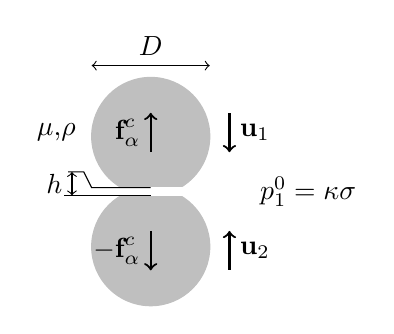
\begin{tikzpicture}
      \draw[lightgray,fill = lightgray] (0,0.7) circle (0.75);
      \draw[lightgray,fill = lightgray] (0,-0.7) circle (0.75);
      \draw[white,fill=white] (-0.75,-0.05) rectangle (0.75,0.05);
      \draw(0,0.05)--++(-0.75,0)--++(-0.1,0.2)--++(-0.2,0);
      \draw(0,-0.05)--++(-1.1,0);
      \draw[<->](-1,-0.05) --++ (0,0.3)node[midway,left]{$h$};
      \draw[<->](-0.75,1.6)--++(1.5,0)node[midway,above]{$D$};
      \node (para) at (-1.2,0.75){$\mu$,$\rho$};
      \node (pressure) at (2,0){$p_1^0 = \kappa \sigma$};
      \draw[->,thick](0,0.5)--++(0,0.5)node[midway,left]{$\textbf{f}_\alpha^\text{c}$};
      \draw[->,thick](0,-0.5)--++(0,-0.5)node[midway,left]{$-\textbf{f}_\alpha^\text{c}$};
      \draw[<-,thick](1,0.5)--++(0,0.5)node[midway,right]{$\textbf{u}_1$};
      \draw[<-,thick](1,-0.5)--++(0,-0.5)node[midway,right]{$\textbf{u}_2$};
    \end{tikzpicture}
    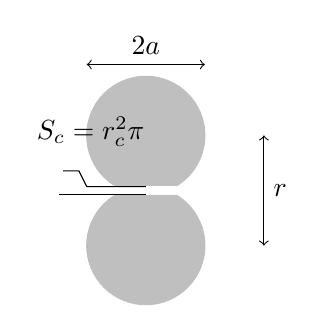
\begin{tikzpicture}
      \draw[lightgray,fill = lightgray] (0,0.7) circle (0.75);
      \draw[lightgray,fill = lightgray] (0,-0.7) circle (0.75);
      \draw[white,fill=white] (-0.75,-0.05) rectangle (0.75,0.05);
      \draw(0,0.05)--++(-0.75,0)--++(-0.1,0.2)--++(-0.2,0);
      \draw(0,-0.05)--++(-1.1,0);
      \draw[<->](-0.75,1.6)--++(1.5,0)node[midway,above]{$2 a$};
      \draw[<->](1.5,0.7)--++(0,-1.4)node[midway,right]{$r$};
      \node (para) at (-0.7,0.75){$S_c = r_c^2 \pi$};
    \end{tikzpicture}
    \caption{Scheme of two colliding droplets at close contact. Note the null kurvature in the region of the interface close to the film leading to a capilary force $\textbf{f}_\alpha^\text{c} \approx - S_c \kappa \sigma \textbf{r}/|\textbf{r}|$. }
\end{figure}

Let use the following notation $(\bm{\sigma}_1' \cdot \textbf{n}_1)^\Sigma = \textbf{f}_\alpha = \textbf{f}_\alpha^\text{h}+\textbf{f}_\alpha^\text{c}$. 
It is clear, since the mean stress contribution $\div \bm{\sigma}_1$ isn't taken in account inside the drag force term, that the contribution $\textbf{f}_\alpha^\text{h}$ vanish or is negligible compared to $\textbf{f}_\alpha^\text{c}$ when the nearest particle is at a distance $|\textbf{r}| < a$ where $a$ is the.  Radius. 

If there is strong inhomogeneous structure in the flow the pure drag force term might be modified to yields the particle fluid particle stress. 
\begin{align*}
    n_p (\bm{\sigma}_1' \cdot \textbf{n}_1)_p^\Sigma
    &= 
    \int_{\mathrm{R}^3} (\bm{\sigma}_1' \cdot \textbf{n}_1)_\text{nst}^\Sigma
    P_\text{nst}(\textbf{x}\pm\textbf{r}/2,\mp\textbf{r}) d\textbf{r}
    +\div \int_{\mathrm{R}^3} \textbf{r} (\bm{\sigma}_1' \cdot \textbf{n}_1)_\text{nst}^\Sigma
    P_\text{nst}(\textbf{x},\textbf{r}) d\textbf{r}\\
\end{align*}
Which can be again decomposed into : 
\begin{align*}
    n_p (\bm{\sigma}_1' \cdot \textbf{n}_1)_p^\Sigma
    &= 
    \frac{1}{2}\int_{\mathrm{R}^3} \textbf{f}^h_\text{nst}P_\text{nst}(\textbf{x}\pm\textbf{r}/2,\mp\textbf{r}) d\textbf{r}
    + \frac{1}{2}\int_{\mathrm{R}^3} \textbf{f}^c_\text{nst}P_\text{nst}(\textbf{x}\pm\textbf{r}/2,\mp\textbf{r}) d\textbf{r} \\
    &
    +\div \int_{\mathrm{R}^3} \textbf{r} \textbf{f}_\text{nst}^\text{h} P_\text{nst}(\textbf{x},\textbf{r}) d\textbf{r}
    +\div \int_{\mathrm{R}^3} \textbf{r} \textbf{f}_\text{nst}^\text{c} P_\text{nst}(\textbf{x},\textbf{r}) d\textbf{r}\\
\end{align*}
The first term is the pure drag force components. 
The second terms is the pure contact force components which we will see to be null in the next section. 
Then, the third term is the particle-fluid-particle stress. 
And the last is the particle-film-particle stress. 


\subsubsection*{The contact forces}
In the same spirit as the classical surface force, as it is defined in \citet{jackson1997locally,zhang1997momentum,nott2011suspension} we can argue that the ensemble average of the close contact force cancel out. 
More precisely, the contact force on a single particle labeled $i$ due to the close contact with particle $j$ can be modeled by, 
\begin{equation*}
    \textbf{f}_{ij}^\text{c}
    = S_c \kappa \sigma \textbf{r}_{ij}/r_{ij}
    = \pi r_c^2 \kappa \sigma \textbf{r}_{ij}/r_{ij}
    = \pi (a^2 - r_{ij}^2/4) \kappa \sigma  \textbf{r}_{ij}/r_{ij}
\end{equation*} 
The resultants of these forces on the particle $i$ is therefore the sum of the contact with all particles except the $j^\text{th}$ particle, 
\begin{equation*}
    \textbf{f}_{i}^\text{c}
    = \sum_{j \neq i}\textbf{f}_{ij}
    = - \sum_{j \neq i} \pi (a^2 - r_{ij}^2/4) \kappa \sigma \textbf{r}_{ij}/r_{ij}
\end{equation*} 
The ensemble average of this force can be written using the classic point particle average,
\begin{align}    
\pavg{\textbf{f}_i^c}
&=
\int \sum_{i} \delta_i 
\textbf{f}_i^c d\PP 
= \int \sum_{i} \sum_{j \neq i} \delta(\textbf{x} - \textbf{x}_i) 
\textbf{f}_{ij}^c d\PP 
\\
\end{align}
Not that $\textbf{f}_{ij} = - \textbf{f}_{ji}$ however $\delta_i \textbf{f}_{ij} \neq - \delta_j\textbf{f}_{ji}$ thus the sum dosen't cancel drictly. 
Thus, following \citet{nott2011suspension,zhang1997momentum} we introduce the sum $\sum_j \delta(\textbf{x}-\textbf{x}_{ij}) \textbf{f}_{ij}^c =0$ where $\textbf{x}_{ij} = \textbf{x}_{ji} = (\textbf{x}_i+\textbf{x}_j)/2$.
Besides, note that, 
\begin{equation*}
    \delta(\textbf{x} - \textbf{x}_{ij})
    = 
    \delta(\textbf{x} - \textbf{x}_i + ( \textbf{x}_{ij} - \textbf{x}_i))
    =
    \delta(\textbf{x} - \textbf{x}_i )
    - ( \textbf{x}_{ij} - \textbf{x}_i)\cdot \grad \delta(\textbf{x}-\textbf{x}_\alpha)
    +\frac{1}{2} (\textbf{x}_{ij} - \textbf{x}_i)(\textbf{x}_{ij} - \textbf{x}_i) : \grad\grad \delta(\textbf{x}-\textbf{x}_\alpha)
\end{equation*}
using both relation yields, 
\begin{align}    
    \pavg{\textbf{f}_i^c}
    &= \int \sum_{i} \sum_{j \neq i} [
        \delta(\textbf{x} - \textbf{x}_i)
        -\delta(\textbf{x} - \textbf{x}_{ij})]
    \textbf{f}_{ij}^c d\PP 
    \\
    &= \div \int \sum_{i} \sum_{j \neq i} \delta(\textbf{x}-\textbf{x}_i) (\textbf{x}_{ij} - \textbf{x}_i)
    \textbf{f}_{ij}^c d\PP 
    \\
    &= \frac{1}{2}\div \int \sum_{i} \sum_{j \neq i} \delta(\textbf{x}-\textbf{x}_i) (\textbf{x}_{j} - \textbf{x}_i)
    \textbf{f}_{ij}^c d\PP 
\end{align}
Using the formula for the contact force gives 
\begin{align}    
    \pavg{\textbf{f}_i^c}
    &= \frac{1}{2}\div \int \sum_{i} \sum_{j \neq i} \delta(\textbf{x}-\textbf{x}_i) 
    \textbf{r}\textbf{r}
    \pi (r^2/4 - a^2) /r \kappa \sigma d\PP 
    \\
\end{align}


\subsubsection*{Nearest stats for contacts forces in dilute case}
In the dilute case we consider only one conatc force so that, 
\begin{equation}
    n_p \textbf{f}^c_p = \iint 
    \sum_i 
    \delta(\textbf{x} -\textbf{x}_i)
    \sum_k 
    \textbf{f}_{k \to i}^\text{c} 
    \sum_{j\neq i}
    \delta(\textbf{x} + \textbf{r} -\textbf{x}_j) h_{ij}(t,\CC)
    d\PP d\textbf{r}\\
\end{equation}
Now we make use of a trick to cancel the pair particles forces by notticing that, 
\begin{equation}
    n_p \textbf{f}^c_p = \iint 
    \sum_k 
    \delta(\textbf{x} -\textbf{x}_k)
    \sum_i
    \textbf{f}_{i\to k}^\text{c} 
    \sum_{j\neq k}
    \delta(\textbf{x} + \textbf{r} -\textbf{x}_j) h_{kj}(t,\CC)
    d\PP d\textbf{r}\\
\end{equation}
So, we have, 
\begin{equation}
    n_p \textbf{f}^c_p = \frac{1}{2}\iint 
    \sum_i 
    \sum_k 
    \left[
        \sum_{j\neq i}
        \delta(\textbf{x} -\textbf{x}_i)
        \delta(\textbf{x} + \textbf{r} -\textbf{x}_j) h_{ij}
        \textbf{f}_{k \to i}^\text{c} 
        +
        \sum_{j\neq k}
        \delta(\textbf{x} -\textbf{x}_k)
        \delta(\textbf{x} + \textbf{r} -\textbf{x}_j) h_{kj}
        \textbf{f}_{i \to k}^\text{c} 
    \right]
    d\PP d\textbf{r}\\
\end{equation}
Note that the sums do not have the same restrictions. 
Nevertheless, this can be neglected since, if for example, $j=i$ we obtain $\delta(\textbf{x}-\textbf{x}_i)\delta(\textbf{x}+\textbf{r}-\textbf{x}_i) = 0$ thus the term cancel unless $\textbf{r}=0$ but let neglect that.
Besides, we must define manually that $h_{ii} = 0$ but it doesn't really matter.   
Or we get out these specifics case such as,
\begin{align}
    n_p \textbf{f}^c_p 
    &= \frac{1}{2}\iint 
    \sum_i 
    \sum_k 
    \sum_{j\neq k,i}
    \left[
        \delta(\textbf{x} -\textbf{x}_i)
        \delta(\textbf{x} + \textbf{r} -\textbf{x}_j) h_{ij}
        \textbf{f}_{k \to i}^\text{c} 
        +
        \delta(\textbf{x} -\textbf{x}_k)
        \delta(\textbf{x} + \textbf{r} -\textbf{x}_j) h_{kj}
        \textbf{f}_{i \to k}^\text{c} 
    \right]
    d\PP d\textbf{r}\\
    &+ \frac{1}{2}\iint 
    \sum_i 
    \sum_k 
    \left[
        \delta(\textbf{x} -\textbf{x}_i)
        \delta(\textbf{x} + \textbf{r} -\textbf{x}_k) h_{ik}
        \textbf{f}_{k \to i}^\text{c} 
        +
        \delta(\textbf{x} -\textbf{x}_k)
        \delta(\textbf{x} + \textbf{r} -\textbf{x}_i) h_{ki}
        \textbf{f}_{i \to k}^\text{c} 
    \right]
    d\PP d\textbf{r}\\
\end{align}

Now we must verify that this framework is coherent with the nearest particle statistics framework.
First we recall the definition of the pure drag term of the contact forces according to the neaerst particle statistics. 
\begin{align*}
    \pavg{\textbf{f}_i^\text{c}}
    &= \frac{1}{2}\int \nstavg{\textbf{f}_i^\text{c}} P_\text{nst}(\textbf{x}\pm\textbf{r}/2,\mp \textbf{r}) d\textbf{r}\\
    &=
    \frac{1}{2}\iint \sum_i \sum_{j\neq i}
    \delta(\textbf{x} \pm \textbf{r}/2 -\textbf{x}_i) 
    \delta(\textbf{x} \mp \textbf{r} -\textbf{x}_j) h_{ij}
    \textbf{f}_i^\text{c} 
    d\PP d\textbf{r}\\
    &=
    \frac{1}{2}\iint \sum_i \sum_{j\neq i}
    \delta(\textbf{x} \pm \textbf{r}/2 -\textbf{x}_i)
    \delta(\textbf{x} \mp \textbf{r} -\textbf{x}_j) h_{ij}
    \sum_{k} \textbf{f}_{ik}^\text{c} 
    d\PP d\textbf{r}\\
    &=
    \frac{1}{2}\iint \sum_i \sum_{j\neq i}
    \delta(\textbf{x} \pm \textbf{r}/2 -\textbf{x}_i)
    \delta(\textbf{x} \mp \textbf{r} -\textbf{x}_j) h_{ij}
     (\textbf{f}_{ij}^\text{c} + \sum_{k\neq i,j} \textbf{f}_{ik}^c)
    d\PP d\textbf{r}
\end{align*}
We must verify that both component of this integral cancel out. 
Changing teh integration sign we get,
\begin{equation*}
    \int \nstavg{\textbf{f}_i^\text{c}} P_\text{nst}(\textbf{x}, \textbf{r}) d\textbf{r}
    = \int \nstavg{\textbf{f}_i^\text{c}} P_\text{nst}(\textbf{x}, - \textbf{r}) d\textbf{r}
\end{equation*}
The drag force can alse, be written, 
\begin{equation*}
    \int [\textbf{f}^c_\text{eb}(\textbf{x}+\textbf{r}/2,\textbf{x} - \textbf{r}/2)+ \textbf{f}_\text{eb}^c(\textbf{x} -\textbf{r}/2,\textbf{x}+ \textbf{r}/2)]P_2(\textbf{x}\pm\textbf{r}/2,\textbf{x}\mp \textbf{r}/2) d\textbf{r}
    = \\
\end{equation*}
And since the contact force has only an antisymmetric contribution in average it is always true that in an averaged sense we have $\nstavg{\textbf{f}_i^\text{c}} P_\text{nst}(\textbf{x}, \textbf{r})  = - \nstavg{\textbf{f}_i^\text{c}} P_\text{nst}(\textbf{x}, - \textbf{r}) $, 
Additionally, 
\begin{align*}
    \pavg{\textbf{f}_\text{eb}^\text{c}}
    &=
    \frac{1}{2}\iint \sum_i \sum_{j\neq i}
    \delta(\textbf{x} + \textbf{r}/2 -\textbf{x}_i)
    \delta(\textbf{x} - \textbf{r}/2 -\textbf{x}_j) h_{ij}
    \sum_{k \neq i} \textbf{f}_{ik}^\text{c} 
    d\PP d\textbf{r}\\
    &=
    \frac{1}{2}\iint \sum_i \sum_{j\neq i}
    \delta(\textbf{x} + \textbf{r}/2 -\textbf{x}_i)
    \delta(\textbf{x} - \textbf{r}/2 -\textbf{x}_j) 
    h_{ij}
    \sum_{k \neq i} \textbf{f}_{ik}^\text{c} 
    d\PP d\textbf{r}\\
\end{align*}

\begin{align}    
\pavg{\textbf{f}_i^c}
&= \int_{|\textbf{r}|<a}
\int \sum_{i \neq j} \delta_i \sum_{j\neq i} \delta_j h_{ij}
\textbf{f}_i^c d\PP d\textbf{r}
= \int_{|\textbf{r}|<a}
\int \sum_{i \neq j} \delta_i \sum_{j\neq i} \delta_j h_{ij}
\sum_{k\neq i} \pi (r_{ik}^2/4 - a^2) \kappa \sigma \textbf{r}_{ik}/r_{ik} d\PP d\textbf{r}\\
&= \int_{|\textbf{r}|<a}
\int \sum_{i \neq j} \delta_i \sum_{j\neq i} \delta_j h_{ij}
\sum_{k\neq i} \pi (r_{ik}^2/4 - a^2) \kappa \sigma \textbf{r}_{ik}/r_{ik} d\PP d\textbf{r}
\\
\end{align}

Anyhow if we lake the assumption that this term indeed cancel we arrive at the expression: 
\begin{equation*}
    \int_{\mathrm{R}^3} \textbf{r} \textbf{f}_\text{nst}^\text{c} P_\text{nst}(\textbf{x},\textbf{r}) d\textbf{r}
    = 
\end{equation*}

\section{The dumping model}

Let decompose the drag force such that $\textbf{f}_\alpha = \textbf{f}_\alpha^h + \textbf{f}_\alpha^c$ with $^h$ being the hydrodynamical forces and $\textbf{f}^c_\alpha$ being the contatc forces. 
Let assume that the particle $\alpha$ interact with the particle $\beta$, where both particles has a radius $a$.
Let note $\textbf{r} = (\textbf{x}_\alpha - \textbf{x}_\beta) = \textbf{n} a$. 
Now let consider that the contact force can be modeled as a spring/dumping model with $k$ being the \textit{Raideur} and $c$ the dumping coefficient.
Then, the contact force between both particles can be written as, 
\begin{equation}
    \textbf{f}_\beta^c
    = \textbf{f}_{\alpha\beta}
    = (|\textbf{r}| - a) \textbf{n} k 
    + (\textbf{u}_\alpha - \textbf{u}_\beta) c
    \;\;\;\;\text{for} \;\;\; (|\textbf{r}| - a) < 0
\end{equation}
For smooth particle the second term can be reduced to the components along the normal vector \textbf{n}.  
Due to Newton's  law and since each interaction force cancel each other we have $\avg{\textbf{f}_\beta^c} \approx 0$. 
However, it is useful to note that we have in the case of inhomogeneous scenario $\avg{\textbf{f}_\beta^c} \approx - \div \Sigma^c$.

Now let's focus on the source term of the granular temperature $\avg{\textbf{f}_\alpha\cdot \textbf{u}_\alpha'} = \avg{\textbf{f}_\alpha^h \cdot \textbf{u}_\alpha'} + \avg{\textbf{f}_\alpha^c\cdot \textbf{u}_\alpha'}$. 
The first source term $\avg{\textbf{f}_\alpha^h \cdot \textbf{u}_\alpha'} \sim k_p$ since $\textbf{f}_\alpha \sim \textbf{u}_\alpha$.

The part due to collision can be re written using the nearest averaged statistics formalism, 
\begin{align*}
    \avg{\textbf{f}_\alpha^c\cdot \textbf{u}_\alpha'}
    &= \int_{\textsc{R}^3}
    \int \sum_{\alpha \neq \beta} \delta_\alpha \delta_\beta h_{\alpha\beta}
    \textbf{u}'_\alpha \textbf{f}_\alpha^c d\PP d\textbf{r}\\
    &= \int_{\textsc{R}^3}
    \int \sum_{\alpha \neq \beta} \delta_\alpha \delta_\beta h_{\alpha\beta}
    \textbf{u}'_\alpha \cdot \textbf{n}
        (|\textbf{r}| - a) 
     d\PP d\textbf{r}
    + \int_{\textsc{R}^3}
    \int \sum_{\alpha \neq \beta} \delta_\alpha \delta_\beta h_{\alpha\beta}
    \textbf{u}'_\alpha 
         (\textbf{u}_\alpha - \textbf{u}_\beta) c
     d\PP d\textbf{r}\\
    &=k \int_{|\textbf{r}|<a}
    \nstavg{\textbf{u}'_\alpha \cdot \textbf{n}
        (|\textbf{r}| - a)   }
        P_{nst}(\textbf{x},\textbf{r})
     d\textbf{r}
    +c \int_{|\textbf{r}|<a}
        \nstavg{\textbf{u}'_\alpha 
         \cdot (\textbf{u}_\alpha - \textbf{u}_\beta)} P_\text{nst}(\textbf{x},\textbf{r})
     d\textbf{r}\\
\end{align*}
Elastic collisions are not dissipative therefore the first term cancel by definition. 
Thus, we are left with, 
\begin{align*}
    \avg{\textbf{f}_\alpha^c\cdot \textbf{u}_\alpha'}
    = c \int_{|\textbf{r}|<a}
        \nstavg{\textbf{u}'_\alpha 
         \cdot (\textbf{u}_\alpha - \textbf{u}_\beta)} P_\text{nst}(\textbf{x},\textbf{r})
     d\textbf{r} 
\end{align*}
\subsection{The dispersed phase equations}

Regarding the dispersed phase, we found the mass, momentum and total energy balance equations, 
\begin{align*}
    \pddt \left(n_p m_p\right)
    + \div \left(n_pm_p\textbf{u}_p
    \right)
    = 
    0\\
    \pddt \left(n_p m_p \textbf{u}_p\right)
    + \div \left(n_p
    m_p \textbf{u}_p \textbf{u}_p 
    - \bm{\sigma}_p^\text{eq}
    \right)
    = 
    n_p v_p  (  
    \rho_2 \textbf{g}
    - \grad p_1)
    + n_p (\bm{\sigma}_1'\cdot \textbf{n}_2)_p^\Sigma,\\
    \pddt(m_p n_pE_p^\text{tot})
    + \div(m_pn_p E_p^\text{tot} \textbf{u}_p 
    + \textbf{q}_p^\text{eq} - \textbf{u}_p \cdot \bm{\sigma}_p^\text{eq})
    =  n_p v_p [\rho_2 \textbf{u}_p\cdot  \textbf{g} 
    - \div (\textbf{u}_1 p_1)]\\
    +  n_p ( \textbf{u}'_1 \cdot \bm{\sigma}_1^0 \cdot \textbf{n}_2)_p^\Sigma
    -  n_p (\textbf{q}_1^0 \cdot \textbf{n}_2)_p^\Sigma
    +  n_p (\textbf{u}_1 \cdot \bm{\sigma}_1'\cdot \textbf{n}_2)_p^\Sigma
\end{align*}
where we have defined, 
\begin{align*}
    &\bm{\sigma}_p^\text{eq}
    = -  m_p\pnavg{\textbf{u}_\alpha'\textbf{u}_\alpha'}
    &\textbf{q}_p^\text{eq}
    =\textbf{q}_p^\text{e} 
    +\textbf{q}_p^\text{k}  
    +\textbf{q}_p^\text{w}  
    \\
    &\textbf{q}_1^\text{e}
    = m_p \pnavg{\textbf{u}_\alpha' e_\alpha'} 
    &\textbf{q}_p^\text{k}
    = m_p \pnavg{\textbf{u}_\alpha' k_\alpha} 
    \\
    &\textbf{q}_p^\text{w}
    = 
    + \pnavg{\textbf{u}_\alpha'(\rho_2 (w^0_2)^2/2 )'_\Omega}
    + \gamma \pnavg{\textbf{u}_\alpha' s_\alpha'}
\end{align*}

Now, subtracting each of these equations to the total NRJ equations yields, 


\tb{Think about doing a surface equation ? ? }
At the Lagrangian scale, 
\begin{equation*}
    \pavg{\ddt (m_\alpha E_\alpha + s_\alpha \gamma)}
    = 
     n_p (\rho_2 \textbf{u}_2^0  \cdot \textbf{g})^\Omega_p
    +n_p (\textbf{u}_1^0 \cdot \bm{\sigma}_1^0 \cdot  \textbf{n}_2)^\Sigma_p
    - n_p (\textbf{q}_1^0 \cdot \textbf{n}_2)^\Sigma_p
\end{equation*}
\begin{align}
    \pavg{\frac{1}{2}\ddt (m_\alpha u_\alpha^2)}
    &= 
    n_p (\rho_2 \textbf{u}_2^0 \cdot
    \textbf{g})_p^\Omega
    + 
    (\textbf{u}_\alpha\cdot
    \textbf{f}_\alpha)_p\\
    \pavg{\frac{1}{2}\ddt \left[\int_{\Omega_\alpha} \rho_2 (w_2^0)^2 d\Omega +s_\alpha \gamma\right] }
    &= (\textbf{w}_1^0 \cdot (\bm{\sigma}_1^0 \cdot \textbf{n}_2) )_p^\Sigma  
     - (\bm{\sigma}_2^0 : \grad\textbf{u}_2^0)_p^\Omega  
    \\
    \pavg{\ddt (m_\alpha e_\alpha )}
    &= 
     + n_p (\bm{\sigma}_2^0 : \grad\textbf{u}_2^0)^\Omega_p
    -  n_p (\textbf{q}_1^0 \cdot \textbf{n}_2 )_p^\Sigma
\end{align}
We first note that, 
\begin{equation*}
    n_p\frac{1}{2}(m_\alpha u_\alpha^2)_p
    = n_p\frac{1}{2}m_p u_p^2
    +  k_p
\end{equation*}
Deriving the momentum kinetic NRJ equation for the particle phase and the above else we can have the following system of equations. 
\begin{align*}
    &\pddt \left(n_p m_p u_p^2/ 2\right)
    + \div \left(n_p
    m_p u_p^2/ 2 \textbf{u}_p 
    - \textbf{u}_p \cdot \bm{\sigma}_p^\text{eq}
    \right)
    = 
    - \bm{\sigma}_p^\text{eq}  :\grad \textbf{u}_p
    +  n_p v_p \textbf{u}_p \cdot (
    \rho_2 \textbf{g}
    - \grad p_1 )
    + n_p \textbf{u}_p \cdot (\bm{\sigma}'_1 \cdot \textbf{n}_2)^\Sigma_p,\\
    &\pddt \left(n_p (\rho_2 w^2 )_p^\Omega+\gamma s_p n_p\right)
    + \div 
    (n_p (\rho_2 w^2 )_p^\Omega+\gamma s_p n_p)
    \textbf{u}_p 
    +  \textbf{q}_p^\text{w}
    )
    = \\
    &- n_p (\bm{\sigma}_2^0 : \grad\textbf{u}_2^0)^\Omega_p
    + n_p (\textbf{u}_1 \cdot \bm{\sigma}_1' \cdot  \textbf{n}_2)^\Sigma_p
    + n_p (\textbf{u}_1' \cdot \bm{\sigma}_1^0 \cdot  \textbf{n}_2)^\Sigma_p
    -n_p v_p \grad (\textbf{u}_1p_1)
    - n_p (\textbf{u}_\alpha \cdot \bm{\sigma}_1^0 \cdot  \textbf{n}_2)^\Sigma_p
    \\
    &\pddt \left(n_p m_p e_p\right)
    + \div \left(n_p
    m_p e_p \textbf{u}_p 
    +  \textbf{q}_p^\text{e}
    \right)
    = 
    + n_p (\bm{\sigma}_2^0 : \grad\textbf{u}_2^0)^\Omega_p
    - n_p (\textbf{q}_1^0\cdot \textbf{n}_2)^\Sigma_p\\
\end{align*}

Now if we subtract these from the total NRJ equation one can show, 
\begin{multline*}
    \pddt(m_p n_pk_p)
    + \div(m_pn_p k_p \textbf{u}_p 
    + \textbf{q}_p^\text{k})
    = 
     \bm{\sigma}_p^\text{eq}  :\grad \textbf{u}_p
     + n_p v_p \textbf{u}_p \grad p_1
     + n_p (\textbf{u}_\alpha \cdot \bm{\sigma}_1^0 \cdot  \textbf{n}_2)^\Sigma_p
     - n_p \textbf{u}_p \cdot (\bm{\sigma}_1' \cdot  \textbf{n}_2)^\Sigma_p
    \\
\end{multline*}
Note that, 















In order to be consistent with the fluid phase equations these terms must be written with $\textbf{f}_\text{pm} = n_p\textbf{u}_1 \cdot ((\bm{\sigma}_1^0 \cdot  \textbf{n}_2)^\Sigma_{nst}(\textbf{x} \pm \textbf{r}/2,\mp\textbf{r}) )_p$, and espetially  $\textbf{f}_\text{pm} = n_p ((\textbf{u}_1' \cdot\bm{\sigma}_1^0 \cdot  \textbf{n}_2)^\Sigma_{nst}(\textbf{x} \pm \textbf{r}/2,\pm\textbf{r}))_p$. Thus we need to reformulate. 
We use, 
\begin{align*}
    n_p (\bm{\sigma}_1^0 \cdot  \textbf{n}_2)^\Sigma_p
    = 
    n_p ( \bm{\sigma}_1' \cdot  \textbf{n}_2)^\Sigma_p
    - n_p (p_1   \textbf{n}_2)^\Sigma_p\\
    n_p (\textbf{u}_1^0 \cdot \bm{\sigma}_1^0 \cdot  \textbf{n}_2)^\Sigma_p
    = 
    n_p (\textbf{u}_1 \cdot \bm{\sigma}_1' \cdot  \textbf{n}_2)^\Sigma_p
    + n_p (\textbf{u}_1' \cdot \bm{\sigma}_1^0 \cdot  \textbf{n}_2)^\Sigma_p
    - n_p (\textbf{u}_1 p_1 \cdot  \textbf{n}_2)^\Sigma_p
\end{align*}
Note that $\textbf{u}_1$ and $p_1$ varies slowly inside the volume of the particle.
Consequently we must use the relation, $\textbf{u}_1(\textbf{r}) = \textbf{u}_1(\textbf{x}_\alpha) + \textbf{r} \cdot\grad \textbf{u}_1(\textbf{x}_\alpha) \ldots$
and $p_1(\textbf{r}) = p_1(\textbf{x}_\alpha) + \textbf{r} \cdot\grad p_1(\textbf{x}_\alpha) \ldots$
to finnaly obtain, 
\begin{align*}
    n_p (\bm{\sigma}_1^0 \cdot  \textbf{n}_2)^\Sigma_p
    &= 
    n_p ( \bm{\sigma}_1' \cdot  \textbf{n}_2)^\Sigma_p
    - n_p v_p \grad p_1\\
    n_p (\textbf{u}_1^0 \cdot \bm{\sigma}_1^0 \cdot  \textbf{n}_2)^\Sigma_p
    &= 
    n_p (\textbf{u}_1 \cdot \bm{\sigma}_1' \cdot  \textbf{n}_2)^\Sigma_p
    + n_p (\textbf{u}_1' \cdot \bm{\sigma}_1^0 \cdot  \textbf{n}_2)^\Sigma_p
    - n_p v_p \div (\textbf{u}_1 p_1) \\
    &= 
    n_p \textbf{u}_1 \cdot( \bm{\sigma}_1' \cdot  \textbf{n}_2)^\Sigma_p
    + n_p (\textbf{r} \bm{\sigma}_1' \cdot  \textbf{n}_2)^\Sigma_p : \grad \textbf{u}_1
    + n_p (\textbf{u}_1' \cdot \bm{\sigma}_1^0 \cdot  \textbf{n}_2)^\Sigma_p
    - n_p v_p \div (\textbf{u}_1 p_1) \\
    &= 
    n_p \textbf{u}_1 \cdot \textbf{f}_{pm}
    + n_p (\mathcal{F}_p - \mathcal{F}_\text{pfp}): \grad \textbf{u}_1
    + n_p \textbf{c}_\text{pm}
    + \div [n_p(\mathcal{C}_\text{pfp} + \textbf{u}_1 \cdot \mathcal{F}_\text{pfp})]
    - n_p v_p \div (\textbf{u}_1 p_1) 
\end{align*}

\begin{align*}
    n_p (\textbf{w}_1^0 \cdot \bm{\sigma}_1^0 \cdot  \textbf{n}_2)^\Sigma_p
    &= 
    n_p (\textbf{u}_1^0 \cdot \bm{\sigma}_1^0 \cdot  \textbf{n}_2)^\Sigma_p
    - n_p (\textbf{u}_\alpha \cdot \bm{\sigma}_1^0 \cdot  \textbf{n}_2)^\Sigma_p\\
    n_p (\textbf{u}_\alpha \cdot \bm{\sigma}_1^0 \cdot  \textbf{n}_2)^\Sigma_p
    &=
    n_p (\textbf{u}_\alpha \cdot \bm{\sigma}_1' \cdot  \textbf{n}_2)^\Sigma_p
    - n_p (\textbf{u}_\alpha \cdot p_1 \cdot  \textbf{n}_2)^\Sigma_p
    % n_p (\textbf{u}_1 \cdot \bm{\sigma}_1' \cdot  \textbf{n}_2)^\Sigma_p
    % + n_p (\textbf{u}_1' \cdot \bm{\sigma}_1^0 \cdot  \textbf{n}_2)^\Sigma_p
    % - n_p v_p \div (\textbf{u}_1 p_1) \\
\end{align*}

In fact if we start back from the exact relation defined in the continuous pahse we can say that ,
\begin{align*}
    \avg{\delta_I (\bm{\sigma}_1^0 ) \textbf{n}_2} - p_1 \grad \phi_1
    = 
    % \avg{\delta_I (\bm{\sigma}_1^0 + p_1)\cdot \textbf{n}_2}
    % = 
    \avg{\delta_I \bm{\sigma}_1'\cdot \textbf{n}_2}
    \\
    \avg{\delta_I (\textbf{u}_1^0 \cdot\bm{\sigma}_1^0 )} - \textbf{u}_1p_1\cdot \grad \phi_1
    % = \avg{\delta_I (\textbf{u}_1 \cdot \bm{\sigma}_1' + \textbf{u}_1' \cdot \bm{\sigma}_1^0 )\cdot \textbf{n}_2}
    = \textbf{u}_1 \cdot \avg{\delta_I \bm{\sigma}_1'\cdot \textbf{n}_2}
    + \avg{\delta_I (\textbf{u}_1' \cdot \bm{\sigma}_1^0 )\cdot \textbf{n}_2}
\end{align*}

incoherence in teh exchange terms, 
\begin{align*}
    n_p (\textbf{u}_\alpha' \cdot \bm{\sigma}_1^0\cdot \textbf{n}_2)^\Sigma_p
    &= \int
    \sum_\alpha \delta_\alpha(\textbf{x} - \textbf{x}_\alpha)
    \textbf{u}_\alpha'(\CC,t)\cdot
    \left[\int_{\Sigma_\alpha} 
     (\bm{\sigma}_1^0 +p_1 \textbf{I})\cdot \textbf{n}_2
     d\textbf{r}
    - \int_{\Sigma_\alpha} 
     p_1  \textbf{n}_2
     d\textbf{r}\right]
     d\PP \\
    &= \int
    \sum_\alpha \delta_\alpha(\textbf{x} - \textbf{x}_\alpha)
    \textbf{u}_\alpha'(\CC,t)\cdot
    \left[\int_{\Sigma_\alpha} 
     \bm{\sigma}_1' +\cdot \textbf{n}_2
     d\textbf{r}
    - v_\alpha \grad p_1(\textbf{x}_\alpha)
    \right]
     d\PP \\
    &= n_p (\textbf{u}_\alpha' \cdot (\bm{\sigma}'_1\cdot \textbf{n}_2)^\Sigma )_p
    -  n_p (\textbf{u}_\alpha' v_p \cdot \grad p_1 )_p
     \\
    &= n_p (\textbf{u}_\alpha' \cdot (\bm{\sigma}'_1\cdot \textbf{n}_2)^\Sigma )_p
     \\
\end{align*}
Since $\textbf{u}_p$ is an Eulerian fields it must be evaluated at $\textbf{r}$ Therefore it must get out the 

Also, 
\begin{align*}
    n_p (\textbf{u}_1' \cdot \bm{\sigma}_1'\cdot \textbf{n}_2)^\Sigma_p
    &= \int
    \sum_\alpha \delta_\alpha(\textbf{x} - \textbf{x}_\alpha)
    \left[\int_{\Sigma_\alpha} 
    \textbf{u}_1'\cdot
    \bm{\sigma}_1^0\cdot \textbf{n}_2
    d\textbf{r}
    + \int_{\Sigma_\alpha} 
    \textbf{u}_1'\cdot
     p_1  \textbf{n}_2
     d\textbf{r}\right]
     d\PP \\
    &= n_p (\textbf{u}_1' \cdot \bm{\sigma}_1^0 \cdot \textbf{n}_2)^\Sigma_p
    -  n_p (\textbf{u}_1'[p_1  +  \textbf{r}\cdot \grad p_1 ]\cdot \textbf{n}_2 )_p^\Sigma
     \\
    &= n_p (\textbf{u}_1' \cdot \bm{\sigma}_1^0 \cdot \textbf{n}_2)^\Sigma_p
    -  n_p p_1  (\div \textbf{u}_1')_p^\Omega
    -  n_p (\textbf{u}_1'[p_1  +  \textbf{r}\cdot \grad p_1 ]\cdot \textbf{n}_2 )_p^\Sigma\\
    &= n_p (\textbf{u}_1' \cdot \bm{\sigma}_1^0 \cdot \textbf{n}_2)^\Sigma_p
    -  n_p\grad p_1\cdot ( \textbf{u}'_1)_p^\Omega
     \\
\end{align*}

Also, 
\begin{align*}
    n_p (\textbf{w}_2^0 \cdot \bm{\sigma}_1^0\cdot \textbf{n}_2)^\Sigma_p
    &= \int
    \sum_\alpha \delta_\alpha(\textbf{x} - \textbf{x}_\alpha)
    \cdot
    \left[\int_{\Sigma_\alpha} 
     \textbf{w}_2^0 (\bm{\sigma}_1^0 +p_1 \textbf{I})\cdot \textbf{n}_2
     d\textbf{r}
    - \int_{\Sigma_\alpha} 
     \textbf{w}_2^0 p_1  \textbf{n}_2
     d\textbf{r}\right]
     d\PP \\
    &= \int
    \sum_\alpha \delta_\alpha(\textbf{x} - \textbf{x}_\alpha)
    \left[\int_{\Sigma_\alpha} 
     \textbf{w}_2^0 \cdot \bm{\sigma}_1'\cdot \textbf{n}_2
     d\textbf{r}
    - \int_{\Sigma_\alpha} 
     \textbf{w}_2^0 (p_1 + \textbf{r}\grad p_1)   \textbf{n}_2
     d\textbf{r}\right]
     d\PP \\
     &= n_p (\textbf{w}_2^0 \cdot \bm{\sigma}_1' \cdot \textbf{n}_2)^\Sigma_p
    - n_p (p_1 \textbf{w}_2^0 \cdot \textbf{n}_2)^\Sigma_p\\
     &= n_p (\textbf{w}_2^0 \cdot \bm{\sigma}_1' \cdot \textbf{n}_2)^\Sigma_p
    - n_p (p_1 (\textbf{w}_2^0 \cdot \textbf{n}_2)^\Sigma)_p
    - n_p (\grad p_1\cdot ( \textbf{r} \textbf{w}_2^0 \cdot \textbf{n}_2)^\Sigma)_p\\
     &= n_p (\textbf{w}_2^0 \cdot \bm{\sigma}_1' \cdot \textbf{n}_2)^\Sigma_p
    - n_p (\grad p_1\cdot ( \div(\textbf{r} \textbf{w}_2^0))^\Omega)_p\\
     &= n_p (\textbf{w}_2^0 \cdot \bm{\sigma}_1' \cdot \textbf{n}_2)^\Sigma_p
    - n_p (\grad p_1\cdot ( \div\textbf{r} \textbf{w}_2^0)^\Omega)_p
    - n_p (\grad p_1\cdot ( \textbf{r} \div\textbf{w}_2^0)^\Omega)_p\\
     &= n_p (\textbf{w}_2^0 \cdot \bm{\sigma}_1' \cdot \textbf{n}_2)^\Sigma_p
\end{align*}







The averaged particle energy $n_p E_p$ can be split into five components,
\begin{equation*}
    n_p m_p E_p(t) 
    = m_p n_p e_p 
    + \pnavg{\int_{\Omega_\alpha(t)} \rho_2  (w_2^0)^2/2 d\Omega}
    + m_p n_p k_p
    + m_p n_p (u_p)^2/2
    + n_p s_p \gamma
    % + \textbf{u}_\alpha \cdot \int_{\Omega_\alpha(t)} \rho_2  \textbf{w}_2^0 d\Omega
\end{equation*}
where $k_p = \pavg{(u_\alpha')^2/2}$.
one equation for each is riquiered 
Using the mass balance and the momentum balance dotted with $\textbf{u}_p$ we obtain the particle kinetic energy balance, 
\begin{align*}
    \pddt \left(n_p m_p u_p^2/ 2\right)
    + \div \left(n_p
    m_p u_p^2/ 2 \textbf{u}_p 
    - \textbf{u}_p \cdot \bm{\sigma}_p^\text{eq}
    \right)
    = 
    - \bm{\sigma}_p^\text{eq}  :\grad \textbf{u}_p
    +  n_p v_p \textbf{u}_p \cdot (
    \rho_2 \textbf{g}
    - \grad p_1 )
    + n_p \textbf{u}_p \cdot \textbf{f}_{pm},\\
    \pddt \left(n_p (\rho_2 w^2 )_p^\Omega+\gamma s_p n_p\right)
    + \div 
    (n_p (\rho_2 w^2 )_p^\Omega+\gamma s_p n_p)
    \textbf{u}_p 
    +  \textbf{q}_p^\text{w}
    )
    = 
    - n_p \textbf{d}_p
    +  n_p (\textbf{u}_1 -\textbf{u}_p) \cdot  (\textbf{f}_{pm} - v_p \grad p_1)
    + n_p\textbf{c}_p\\
    \pddt \left(n_p m_p e_p\right)
    + \div \left(n_p
    m_p e_p \textbf{u}_p 
    +  \textbf{q}_p^\text{e}
    \right)
    = 
    + n_p \textbf{d}_p
    + n_p \textbf{e}_{pm},\\
\end{align*}
\tb{we remark that the collision tensor appear exactly at the same place as the pfp}
Subtracting all 3 equation to the total energy finally gives, 
\begin{align*}
    \pddt(m_p n_pk_p)
    + \div(m_pn_p k_p \textbf{u}_p 
    + \textbf{q}_p^\text{k})
    = 
    \bm{\sigma}_p^\text{eq} : \grad \textbf{u}_p
    % - n_p \textbf{d}_p
    - n_p v_p p_1 \div \textbf{u}_1
    + n_p (( \textbf{u}_\alpha' \cdot \bm{\sigma}_1^0 \cdot \textbf{n}_2)^\Sigma_\text{nst}(\textbf{x}\pm\textbf{r}/2,\mp\textbf{r}) )_p^r \\
\end{align*}
The transfer term of the internal droplets' fluctuation reads, 
\begin{align*}
    \int_{\Sigma_\alpha} \textbf{w}_1^0 \cdot (\bm{\sigma}_1^0 \cdot \textbf{n}_2) d\Sigma  
    = 
    (\textbf{u}_1 -\textbf{u}_\alpha) \cdot \int_{\Sigma_\alpha}  (\bm{\sigma}_1^0 \cdot \textbf{n}_2) d\Sigma  
    + \int_{\Sigma_\alpha} \textbf{u}_1' \cdot (\bm{\sigma}_1^0 \cdot \textbf{n}_2) d\Sigma  
    = (\textbf{u}_1 -\textbf{u}_\alpha) \cdot  (\textbf{f}_\alpha - \grad p_1)
    + \textbf{c}_\alpha
\end{align*}
\begin{align*}
    n_p (\textbf{w}_1^0 \cdot \bm{\sigma}_1^0 \cdot \textbf{n}_2)^\Sigma_p
    &= 
    n_p ((\textbf{w}_1^0 \cdot \bm{\sigma}_1^0 \cdot \textbf{n}_2)^\Sigma_\text{nst}(\textbf{x}\pm\textbf{r}/2,\mp\textbf{r}) )_p^r 
    + \div (n_p ( \textbf{r}(\textbf{w}_1^0 \cdot \bm{\sigma}_1^0 \cdot \textbf{n}_2)^\Sigma_\text{nst}(\textbf{x},\textbf{r}) )_p^r )\\
    &= 
    n_p (((\textbf{u}_1-\textbf{u}_\alpha) \cdot \bm{\sigma}_1^0 \cdot \textbf{n}_2)^\Sigma_\text{nst}(\textbf{x}\pm\textbf{r}/2,\mp\textbf{r}) )_p^r 
    +n_p ((\textbf{u}_1' \cdot \bm{\sigma}_1^0 \cdot \textbf{n}_2)^\Sigma_\text{nst}(\textbf{x}\pm\textbf{r}/2,\mp\textbf{r}) )_p^r \\
    &+ \div [n_p ( \textbf{r}((\textbf{u}_1 - \textbf{u}_\alpha) \cdot \bm{\sigma}_1^0 \cdot \textbf{n}_2)^\Sigma_\text{nst}(\textbf{x},\textbf{r}) )_p^r 
    + n_p ( \textbf{r}(\textbf{u}_1' \cdot \bm{\sigma}_1^0 \cdot \textbf{n}_2)^\Sigma_\text{nst}(\textbf{x},\textbf{r}) )_p^r ]\\
    &= 
    n_p (((\textbf{u}_1-\textbf{u}_\alpha) \cdot \bm{\sigma}_1^0 \cdot \textbf{n}_2)^\Sigma_\text{nst}(\textbf{x}\pm\textbf{r}/2,\mp\textbf{r}) )_p^r 
    +n_p \textbf{c}_{pm} \\
    &+ \div [n_p ( \textbf{r}((\textbf{u}_1 - \textbf{u}_\alpha) \cdot \bm{\sigma}_1^0 \cdot \textbf{n}_2)^\Sigma_\text{nst}(\textbf{x},\textbf{r}) )_p^r 
    + n_p \mathcal{C}_\text{pfp}]\\
\end{align*}
The remaining terms can be expressed as, 
\begin{align*}
    n_p (((\textbf{u}_1-\textbf{u}_\alpha) \cdot \bm{\sigma}_1^0 \cdot \textbf{n}_2)^\Sigma_\text{nst}(\textbf{x}\pm\textbf{r}/2,\mp\textbf{r}) )_p^r 
    &= 
    n_p (\textbf{u}_1 - \textbf{u}_p) \cdot (( \bm{\sigma}_1^0 \cdot \textbf{n}_2)^\Sigma_\text{nst}(\textbf{x}\pm\textbf{r}/2,\mp\textbf{r}) )_p^r \\
    &- n_p (( \textbf{u}_\alpha' \cdot \bm{\sigma}_1^0 \cdot \textbf{n}_2)^\Sigma_\text{nst}(\textbf{x}\pm\textbf{r}/2,\mp\textbf{r}) )_p^r \\
    &= 
    n_p (\textbf{u}_1 - \textbf{u}_p) \cdot(\textbf{f}_p - \grad p_1) \\
    &- n_p (( \textbf{u}_\alpha' \cdot \bm{\sigma}_1^0 \cdot \textbf{n}_2)^\Sigma_\text{nst}(\textbf{x}\pm\textbf{r}/2,\mp\textbf{r}) )_p^r \\
\end{align*}
The higher moments terms can be expressed as, 
\begin{align*}
    n_p (\textbf{r}((\textbf{u}_1-\textbf{u}_\alpha) \cdot \bm{\sigma}_1^0 \cdot \textbf{n}_2)^\Sigma_\text{nst})_p^r 
    &= 
    n_p (\textbf{u}_1 - \textbf{u}_p) \cdot (\textbf{r} ( \bm{\sigma}_1^0 \cdot \textbf{n}_2)^\Sigma_\text{nst} )_p^r 
    - n_p ( \textbf{r} ( \textbf{u}_\alpha' \cdot \bm{\sigma}_1^0 \cdot \textbf{n}_2)^\Sigma_\text{nst} )_p^r \\
    &= 
    n_p (\textbf{u}_1 - \textbf{u}_p)\cdot \mathcal{F}_\text{pfp} 
    - n_p (\textbf{r} ( \textbf{u}_\alpha' \cdot \bm{\sigma}_1^0 \cdot \textbf{n}_2)^\Sigma_\text{nst} )_p^r \\
\end{align*}
Alternatively, without the nearest particle formalism we obtain, 
\begin{align*}
    n_p (\textbf{w}_1^0 \cdot \bm{\sigma}_1^0 \cdot \textbf{n}_2)^\Sigma_p
    &= 
    n_p ((\textbf{w}_1^0 \cdot \bm{\sigma}_1^0 \cdot \textbf{n}_2)^\Sigma)_p 
\end{align*}

Averaging the microscopic 
\begin{align}
    \frac{1}{2}\ddt (m_\alpha u_\alpha^2)
    &= 
    \textbf{u}_\alpha\cdot
    \textbf{g}m_\alpha
    + 
    \textbf{u}_\alpha\cdot
    \textbf{f}_\alpha\\
    \frac{1}{2}\ddt \int_{\Omega_\alpha} \rho_2 (w_2^0)^2 d\Omega 
    + \ddt (s_\alpha \gamma) 
    &= 
    \int_{\Sigma_\alpha} \textbf{w}_1^0 \cdot (\bm{\sigma}_1^0 \cdot \textbf{n}_2) d\Sigma  
     - \int_{\Omega_\alpha} \bm{\sigma}_2^0 : \grad\textbf{u}_2^0 d\Omega  
    \\
    \ddt (m_\alpha e_\alpha )
    &= 
     \int_{\Omega_\alpha} \bm{\sigma}_2^0 : \grad\textbf{u}_2^0 d\Omega  
    -  s_\alpha \textbf{q}_\alpha  
\end{align}
Additionally, we can add an equation for the first moment of momentum, 
\begin{multline}
    \pddt \left(n_p \mathcal{P}_p\right)
    + \div \left(
        n_p \textbf{u}_p \mathcal{P}_p
    + \Sigma_p^\text{eq}
    \right)
    =
    n_p v_p \bm{\sigma}_1 
    + n_p \mathcal{F}_p\\
    +\pnavg{\int_{\Omega_\alpha} \left(
        \rho_2 \textbf{w}_2^0  \textbf{w}_2^0 
        - \bm{\sigma}_2^0
        \right) d\Omega}
        - \gamma  \pnavg{\int_{\Sigma_\alpha} \textbf{I}_{||} d\Sigma},
\end{multline}



\subsubsection{Modeling of collisions}

Even through we do not consider pure contact between interfaces it is still indispensable to define some kind of collision with the framework of the hybrid model. 
A contact mediated by the fluid is still different from near close contact, since in the latter case it is capillary pressure that drives the interaction forces. 

\subsection*{The drag force term}

The drag force term is easily closed by numerical method and some theoretical developments in the limiting case. 
Let now study the stokes 

\subsection*{Stress tensor for the continuous phase }
Regarding the fluid stress it can be reformulated considering Newtonian fluid,
\begin{equation}
    \phi_1 \bm{\sigma}_1 
    = - \phi_1 p_1 \textbf{I}
    + \mu_1 \phi_1 \textbf{e}_1
\end{equation}
with $\textbf{e}_1$ being the averaged shear rate. 
The first model is then, 
\begin{align*}
    \phi_1 \textbf{e}_1
    = \phi_1 (\nabla \textbf{u}_1+ (\grad \textbf{u}_1)^T)
    + \avg{[(\textbf{u}_1^0 - \textbf{u}_1)  \textbf{n}_1 +  \textbf{n}_1(\textbf{u}_1^0 - \textbf{u}_1 )]\delta_I}
\end{align*}
In \citet[chap 9]{ishii1975thermo} they assume,
\begin{equation}
    \avg{[(\textbf{u}_1^0 - \textbf{u}_1)  \textbf{n}_1 +  \textbf{n}_1(\textbf{u}_1^0 - \textbf{u}_1 )]\delta_I}\\
    = 
    (\textbf{u}_2 - \textbf{u}_1)  \grad \phi_1 +  \grad \phi_1(\textbf{u}_2 - \textbf{u}_1 )\\
\end{equation}
But I didn't find out where the derivation came from. 
Alternatively we can say that, 
\begin{align*}
    \phi_1 \textbf{e}_1
    = \nabla \textbf{u}+ (\grad \textbf{u})^T
    - \avg{\chi_2 (\grad\textbf{u}_2^0 + \grad(\textbf{u}_2^0 )^T)}
    = \textbf{e}
    - \phi_2 \textbf{e}_2
\end{align*}

More generally the stress within a suspension can be written,
\begin{align*}
    \bm{\sigma}_1 \phi_1
    &=- \phi_1 p_1 \textbf{I}
    + \mu_1 \textbf{e}
    - \lambda \phi_2 \bm{\tau}_2\\
    \bm{\sigma}_1 
    &= - \left(p_1 + \frac{\lambda \phi_2}{\phi_1} p_2\right) \textbf{I}
    + \frac{\mu_1}{\phi_1} \textbf{e}
    - \frac{\lambda \phi_2}{\phi_1} \bm{\sigma}_2\\
    \bm{\sigma}
    &= - \phi_1 p_1  \textbf{I}
    + \mu_1 \textbf{e}
    + \bm{\sigma}_2 \phi_2 
    +\phi_I \bm{\sigma}_I 
    - \lambda \phi_2 \bm{\tau}_2
\end{align*}
We can reformulate the last expression in the usual way using the first moment of momentum eq, 
\begin{equation}
    -  \dot{\mathcal{P}_p}
    +  \mathscr{S}_p^*
    +  \mathscr{L}_p
    + \frac{1}{3}(\bm{\sigma}_1^0 \cdot \textbf{n}_2 \cdot \textbf{r})_p^\Sigma \textbf{I}
    + n_p (\rho_2 \textbf{w}_2^0  \textbf{w}_2^0 )^\Omega
    =   (\bm{\sigma}_2^0)^\Omega
    + (\bm{\sigma}_I)^\Sigma,
\end{equation}
Or in stokes condition, 
\begin{equation}
    n_p \mathscr{S}_p^*
+ n_p \mathscr{L}_p
+ n_p\frac{1}{3}(\bm{\sigma}_1^0 \cdot \textbf{n}_2 \cdot \textbf{r})_p^\Sigma \textbf{I}
    = n_p \left(
        \bm{\sigma}_2^0
    \right)_p^\Omega
    +n_p (\bm{\sigma}_I)^\Sigma_p
\end{equation}
where we defined, 
\begin{align*}
    \mathscr{S}_p^* =\frac{1}{2} \pnavg{\int_{\Sigma_\alpha} \left(
        \textbf{r} \bm{\sigma}_1^0 \cdot \textbf{n}_2
        +  \bm{\sigma}_1^0 \cdot \textbf{n}_2\textbf{r}
        -
          \frac{2}{3}(\bm{\sigma}_1^0 \cdot \textbf{n}_2 \cdot \textbf{r})\textbf{I}
        \right)  d\Sigma}\\
    \mathscr{L}_p =\frac{1}{2} \pnavg{\int_{\Sigma_\alpha} \left(
        \textbf{r} \bm{\sigma}_1^0 \cdot \textbf{n}_2
        - \bm{\sigma}_1^0 \cdot \textbf{n}_2\textbf{r}
        \right) d\Sigma}
\end{align*}
Thus in homogeneous suspension without inertia we have, 
\begin{align*}
    \bm{\sigma}
    &= [- \phi_1 p_1 
    + n_p (\bm{\sigma}_1^0 \cdot \textbf{n}_2 \cdot \textbf{r})^\Sigma_p] \textbf{I}
    + \mu_1 \textbf{e}
    + n_p \mathscr{S}
    + n_p \mathscr{L}
\end{align*}
where the stress let is defined as $\mathscr{S} = \mathscr{S}_p^* - \lambda \phi_2 \bm{\tau}_2$. 
The equivalent stress in the fluid phase averaged equation can be reformulated as, 
\begin{align*}
    \bm{\sigma}_1^\text{eq}
    = \phi_1(
    \bm{\tau}_1%- n_p \textbf{M}_p
    - \rho_1 
    \kavg{\textbf{u}_1'\textbf{u}_1'})
    - n_p \mathcal{F}_\text{pfp} + n_p \mathcal{F}_p
    &= - (\phi_1 \rho_1  \kavg{\textbf{u}_1'\textbf{u}_1'}
        + n_p \mathcal{F}_\text{pfp})
        + \mu_1 \textbf{e} 
        - \lambda \phi_2 \bm{\tau}_2
         + n_p \mathcal{F}_p\\
    &= - (\phi_1 \rho_1  \kavg{\textbf{u}_1'\textbf{u}_1'}
        + n_p \mathcal{F}_\text{pfp})
        + \mu_1 \textbf{e} 
        - \lambda \phi_2 \bm{\tau}_2
         + n_p \mathscr{S}_p^*
         + n_p \mathscr{L}_p\\
    &= - (\phi_1 \rho_1  \kavg{\textbf{u}_1'\textbf{u}_1'}
        + n_p \mathcal{F}_\text{pfp})
        + \mu_1 \textbf{e} 
         + n_p \mathscr{S}_p
         + n_p \mathscr{L}_p
         + n_p (\bm{\sigma}_1^0 \cdot \textbf{n}_2 \cdot\textbf{r})_p^\Sigma \textbf{I}
\end{align*}
Thus, in the most general way the fluid phase stress can be written as that. 
But the last term must go into the equivalent pressure and that is a major founding. 
For netrally buoyant spherical particles : 
\begin{equation*}
    + n_p (\bm{\sigma}_1^0 \cdot \textbf{n}_2 \cdot\textbf{r})_p^\Sigma \textbf{I}
    = 
    n_p/a (p_1^0 )_p^\Sigma \textbf{I}
\end{equation*}
This, is definitely not trivial but if one wish to compute the first moment dynamical contribution to the suspension the formulas is given by 
\begin{align*}
    n_p \mathscr{S}_p
+ n_p \mathscr{L}_p
+ n_p\frac{1}{3}(\bm{\sigma}_1^0 \cdot \textbf{n}_2 \cdot \textbf{r})_p^\Sigma \textbf{I}
    &= 
    n_p \left(
        \bm{\sigma}_2^0
    \right)_p^\Omega
    +n_p (\bm{\sigma}_I)^\Sigma_p
    - \lambda \phi_2 \bm{\tau}_2\\
    &= 
    - n_p \left(
        p_2^0
    \right)_p^\Omega \textbf{I}
    +n_p (\bm{\sigma}_I)^\Sigma_p
    + n_p (1 - \lambda)\left(
        \mu_2 \textbf{e}_2^0
    \right)_p^\Omega 
\end{align*}
Let take the trace times $\frac{1}{3}$ of this equation, 
\begin{align*}
    \frac{1}{3} n_p(\bm{\sigma}_1^0 \cdot \textbf{n}_2 \cdot \textbf{r})_p^\Sigma 
    = 
    - n_p \left(
        p_2^0
    \right)_p^\Omega 
    +n_p \frac{1}{3}(\bm{\sigma}_I)^\Sigma_p : \textbf{I}
\end{align*}
Now let's substitute this equation into the former one, 
\begin{align*}
    n_p \mathscr{S}_p
+ n_p \mathscr{L}_p
=
    +n_p (\bm{\sigma}_I - \frac{1}{3}(\bm{\sigma}_I : \textbf{I})\text{I})^\Sigma_p
    + n_p (1 - \lambda)\left(
        \mu_2 \textbf{e}_2^0
    \right)_p^\Omega 
\end{align*}

If the particle is spherical, and that we remove the isotropic part on both sides of the equation we obtain 

In the spherical particle case the symmetric part reads, 
\begin{align*}
    n_p \mathscr{S}_p
    &= 
    + n_p (1 - \lambda)\left(
        \mu_2 \textbf{e}_2^0
    \right)_p^\Omega 
\end{align*}
which is false. 

\subsubsection{A translating sphere}
In the dilute stokes regime the disturbance velocity around a droplet can be written, 
\begin{align*}
    u_i^\text{Ext}(\textbf{r})
    = \left(\frac{\delta_{ik}}{r} + \frac{r_ir_k}{r^3}\right)  g_k
    + \left(-\frac{\delta_{ik}}{r^3} + \frac{3r_ir_k}{r^5}\right)  d_k\\
    u_i^\text{In}(\textbf{r})
    = c_i
    + \left(2 r^2 \delta_{ik} - r_ir_k\right) e_k\\
    e_{ik}
    = \mu(
        3 \delta_{ij} r_k 
        + 3 \delta_{kj} r_i
        -2 r_j \delta_{ki}
    )e_j 
\end{align*}
Applying the non deformation at the interface and other shear free condition we find the constant to be, 
\begin{align*}
    &\textbf{g} = \frac{1}{4}\left(\frac{3\lambda + 2}{\lambda +1}\right) a \textbf{U}
    &\textbf{d} = -\frac{1}{4}\left(\frac{\lambda}{\lambda +1}\right) a^3 \textbf{U}\\
    &\textbf{c} = \frac{1}{2}\left(\frac{3\lambda + 3}{\lambda +1}\right) \textbf{U}
    &\textbf{e} = -\frac{1}{2}\left(\frac{1}{\lambda +1}\right) \frac{1}{a^2} \textbf{U}\\
\end{align*}
Let consider isolated particles immersed in a viscous flow in the case $\textbf{u}_1' = \textbf{u}^{Ext}$.

The averaged internal shear rate $\phi_2 \textbf{e}_2$ can be thus estimated through the integral, 
\begin{align*}
    \avg{\chi_2 (\textbf{e}_2^0)_{ik}}
    &= \pavg{\int_{\Omega} \mu(
        3 \delta_{ij} r_k 
        + 3 \delta_{kj} r_i
        -2 r_j \delta_{ki}
    )e_j d\Omega}
    = 0\\
    &+ \div \pavg{\int_{\Omega} \textbf{r}\mu(
        3 \delta_{ij} r_k 
        + 3 \delta_{kj} r_i
        -2 r_j \delta_{ki}
    )e_j d\Omega}
\end{align*}
Also, the stress fields for such a flow is given by, 
\begin{equation*}
    T^G_{ijl} 
    = -6\frac{r_ir_jr_k}{r^5}
\end{equation*}

What about the first moment of momentum of the droplets, 
\begin{align*}
    (\mathcal{P}_p)_{ij}
    = \int_{\Omega} 
    u_i^\text{In} r_j 
    d\Omega
    = \int_{\Omega} 
    (c_i r_j 
    + 2 r^2  r_j e_i - r_i r_k r_j e_k)
    d\Omega
    = 0 
\end{align*}
Where we considered spherical particle with no deformation so it is obviously zero.
\begin{align*}
    (\textbf{w}_2^0 \textbf{w}_2^0)_{ij}^\Omega
    = \int_{\Omega} 
    u_i^\text{In}u_j^\text{In}
    d\Omega
    = \int_{\Omega} 
    ( c_i + \left(2 r^2 \delta_{ik} - r_ir_k\right) e_k)
    ( c_j + \left(2 r^2 \delta_{jl} - r_jr_l\right) e_l)
    d\Omega\\
    = \int_{\Omega} 
    (c_i c_j + c_i e_l (2 r^2 \delta_{jl} - r_jr_l )
    + (2 r^2 \delta_{ik} - r_ir_k)c_j e_k
    +  (2 r^2 \delta_{ik} - r_ir_k)(2 r^2 \delta_{jl} - r_jr_l)e_ke_l
    )
    d\Omega\\
    = c_i c_j v_\alpha
    + e_l c_i (2 \mathcal{M}_{kk} \delta_{jl} - \mathcal{M}_{jl})
    + e_k c_j (2 \mathcal{M}_{kk} \delta_{ik} - \mathcal{M}_{ik})\\
    + e_ke_l (\mathcal{M}_{kkkk}\delta_{ik}\delta_{jl}
    -2\mathcal{M}_{kkjl}\delta_{ik}
    -2\mathcal{M}_{kkik}\delta_{jl}
    + \mathcal{M}_{ikjl}) 
\end{align*}
\tb{problem on the units ; Re compute those Acknowledging that the inertia tensor is in fact completely isotropic}

The iternal energy, 
\begin{align*}
    (\textbf{w}_2^0 \textbf{w}_2^0)_{ii}^\Omega
    = \int_{\Omega} 
    u_i^\text{In}u_i^\text{In}
    d\Omega
    = \int_{\Omega} 
    ( c_i + \left(2 r^2 \delta_{ik} - r_ir_k\right) e_k)
    ( c_i + \left(2 r^2 \delta_{il} - r_ir_l\right) e_l)
    d\Omega\\
    = \int_{\Omega} 
    (c_i c_i + c_i e_l (2 r^2 \delta_{il} - r_ir_l )
    + (2 r^2 \delta_{ik} - r_ir_k)c_i e_k
    +  (2 r^2 \delta_{ik} - r_ir_k)(2 r^2 \delta_{il} - r_ir_l)e_ke_l
    )
    d\Omega\\
    = c_i c_i v_\alpha
    + e_l c_i (2 \mathcal{M}_{kk} \delta_{il} - \mathcal{M}_{il})
    + e_k c_i (2 \mathcal{M}_{kk} \delta_{ik} - \mathcal{M}_{ik})\\
    + e_ke_l (\mathcal{M}_{kkkk}\delta_{ik}\delta_{il}
    -2\mathcal{M}_{kkil}\delta_{ik}
    -2\mathcal{M}_{kkik}\delta_{il}
    + \mathcal{M}_{ikil}) 
\end{align*}


\subsubsection{A drop in shear flow}

The functional form of the internal velocity fields for a droplet immersed in a shear flow is,
\begin{align*}
    u_i^\text{Ext}(\textbf{r})
    = \left(\frac{\delta_{ij} r_l - \delta_{il} r_j - \delta_{jl} r_i}{r^3} 
    + \frac{r_ir_jr_l}{r^5}\right)  d_{jl}\\
    + \left(-3 \frac{\delta_{ij} r_l + \delta_{il} r_j + \delta_{jl} r_i}{r^5} 
    + 15\frac{r_ir_jr_l}{r^7}\right)  p_{jl}\\
    u_i^\text{In}(\textbf{r})
    = \left(- 4 \delta_{ij} r_l  + \delta_{il} r_j + \delta_{jl} r_i\right) f_{jl}\\
    e_{ik}
    = \mu [
        \partial_i \left(- 4 \delta_{kj} r_l  + \delta_{kl} r_j + \delta_{jl} r_k\right) f_{jl} + \partial_k \left(- 4 \delta_{ij} r_l  + \delta_{il} r_j + \delta_{jl} r_i\right) f_{jl} 
    ]\\
    = \mu [
        \left(- 4 \delta_{kj} \delta_{li}  + \delta_{kl} \delta_{ji} + \delta_{jl} \delta_{ki}\right) f_{jl} + \left(- 4 \delta_{ij} \delta_{lk}  + \delta_{il} \delta_{kj} + \delta_{jl} \delta_{ki}\right) f_{jl} 
    ]\\
    = \mu [
        \left(- 4 f_{ki}  + f_{ik} + f_{jj}\delta_{ki}\right)  + \left(- 4 f_{ik}  + f_{ki} + f_{jj} \delta_{ki}\right)  
    ]\\
    = \mu [
        \left(- 3 f_{ki}  - 3 f_{ik} +2 f_{jj}\delta_{ki}\right) 
    ]
\end{align*}
\todo[inline]{include the 3rd order terms to describe the internal flow}
Here i know that, 
\begin{align*}
    \textbf{d}
    = - \frac{1}{6} \left(
        \frac{2+5\lambda}{1+\lambda}a^3 \textbf{E}
    \right)
    &&
    \textbf{p}
    = - \frac{1}{6} \left(
        \frac{\lambda(2+5\lambda)}{(1+\lambda)(5\lambda+2)}a^3 \textbf{E}
    \right)
\end{align*}
Integrating this functional over the volume of a droplet yields, 
\begin{equation}
    \avg{\chi_2 (\textbf{e}_2^0)_{ik}}
    = \pavg{\int_{\Omega} 
        \mu [
        \left(- 3 f_{ki}  - 3 f_{ik} +2 f_{jj}\delta_{ki}\right) 
    ] d\Omega}
    = n_pv_p(-3 (f_{ki}+ f_{ik}) + 2 f_{jj} \delta_{ki})
\end{equation}
The only remaining thing is to do determine the form of $f_{ik}$. 


\subsection*{Continuous phase fluctuation term}

The Reynolds stress $\oneavg{\textbf{u}_1'\textbf{u}_1'}$ can be described in the limit of dilute non interaction particles by the wake. 
Therefore, by direct integration of $\textbf{u}^\text{Ext}$ we should be able to find a first correction of the velocity correlation. 
In a homogeneous flow of isolated particle ensemble average is equivalent to volume average thus, 
\begin{align*}
    \oneavg{\textbf{u}_1' \textbf{u}_1' }
    = \int u_i^\text{Ext} u_j^\text{Ext}(\textbf{x},\textbf{r}) P_1(\textbf{r}) d\textbf{r}\\
    = \int [\left(\frac{\delta_{ik}}{r} + \frac{r_ir_k}{r^3}\right)  g_k
    + \left(-\frac{\delta_{ik}}{r^3} + \frac{3r_ir_k}{r^5}\right)  d_k]
    [ \left(\frac{\delta_{jl}}{r} + \frac{r_jr_l}{r^3}\right)  g_l
    + \left(-\frac{\delta_{jl}}{r^3} + \frac{3r_jr_l}{r^5}\right)  d_l] d\textbf{r}
\end{align*}
The expansion of the fluctuation velocity is, i
\begin{align*}
    (\textbf{u}'_1)_i 
    (\textbf{u}'_1)_j
    &=
    \frac{g_i g_j}{r^{2}} 
    - \frac{d_i g_j}{r^{4}} 
    - \frac{d_j g_i}{r^{4}} 
    + \frac{g_i g_l x_j x_l}{r^{4}} 
    + \frac{g_j g_k x_i x_k}{r^{4}} \\
    &+ \frac{d_i d_j}{r^{6}} 
    - \frac{d_i g_l x_j x_l}{r^{6}} 
    - \frac{d_j g_k x_i x_k}{r^{6}} 
    + \frac{3 d_k g_j x_i x_k}{r^{6}} 
    + \frac{3 d_l g_i x_j x_l}{r^{6}} 
    + \frac{g_k g_l x_i x_j x_k x_l}{r^{6}} \\
    &- \frac{3 d_i d_l x_j x_l}{r^{8}} 
    - \frac{3 d_j d_k x_i x_k}{r^{8}} 
    + \frac{3 d_k g_l x_i x_j x_k x_l}{r^{8}} 
    + \frac{3 d_l g_k x_i x_j x_k x_l}{r^{8}} \\
    &+ \frac{9 d_k d_l x_i x_j x_k x_l}{r^{10}} 
\end{align*}
Since we kwon that this flow is axissymetri ctit can acctually be computed such thta
\begin{align*}
    (\textbf{u}'_1)_k 
    (\textbf{u}'_1)_l
    &= 
    ((\textbf{u}'_1)_i 
    (\textbf{u}'_1)_j p_j p_i) p_k p_l 
    + 
    ((\textbf{u}'_1)_i 
    (\textbf{u}'_1)_j (\delta_{ij} - p_j p_i))(\delta_{kl} -  p_k p_l )\\
    &= 
    ((\textbf{u}'_1)_i 
    (\textbf{u}'_1)_j )_{||} p_k p_l 
    + 
    ((\textbf{u}'_1)_i 
    (\textbf{u}'_1)_j )_{\bot}(\delta_{kl} -  p_k p_l )
\end{align*} 
where \textbf{p} is the normalized vector in the direction of \textbf{U}. 

Each of these terms must be integrated from $a$ to $\infty$ in a spherical coordinate frame. 
In spherical coordinate $d\textbf{r} = r^2 \sin\theta dr d\theta d\phi$. 
In this frame we have $x_0 = r \sin \theta \cos\phi$, $x_1 = r \sin \theta \sin\phi$ and $x_2 = r \cos\theta$.
Therefore, the first integration reads, 
\begin{equation*}
    \int_0^{2\pi} 
    \int_0^{\pi} 
    \int_1^{\infty} 
    \frac{1}{r^2} 
    r^2 \sin\theta dr d\theta d\phi
    = 
    4\pi 
    \int_1^\infty dr
\end{equation*}
This integral diverges thus it is not possibly feasible to compute such thing,
however we can relate the ensemble average to nearest conditional average by the relation : 
\begin{multline*}
    \avg{\chi_k \textbf{u}'_k\textbf{u}'_k}(\textbf{x},t)
    + \phi_k \textbf{u}_k\textbf{u}_k
    = \\
    \underbrace{\int (\nstavg{\chi_k \textbf{u}^0_k}  \nstavg{\chi_k \textbf{u}^0_k} / (\nstavg{\chi_k})  P_{nst}(\textbf{x},t,\textbf{r}) d\textbf{r} }_\text{PWFs}
    +\underbrace{\int \nstavg{\chi_k \textbf{v}_k^0\textbf{v}_k^0}  P_{nst}(\textbf{x},t,\textbf{r}) d\textbf{r}}_\text{WIA}
    \label{eq:def_uu}
\end{multline*}
where, $\textbf{v}_k^0  = \textbf{u}_k^0 - \nstavg{\chi_k \textbf{u}^0_k} / \nstavg{\chi_k}$ 
for a dillute random distribution, $P_\text{nst}^\text{th}(\textbf{y}|\textbf{x}) = n_p e^{-4 \pi n_p (r^3 - a^3)/3}$,

If we consider a flow in the $x$ direction we obtain for the three term sthe following integrands,
\begin{align*}
    \iint (\textbf{u}_1'\textbf{u}_1')_{00} r^2 \sin\theta d\phi d\theta
    = e^{\frac{4 \pi a^{3}}{3}}n_{p} \pi \frac{16}{5}\left(\frac{7   g^{2}_0  }{3} 
    + \frac{2   d_0 g_0 }{3 r^{2}} 
    + \frac{   d^{2}_0 }{ r^{4}} \right)e^{- \frac{4 \pi r^{3}}{3}}\\
    \iint (\textbf{u}_1'\textbf{u}_1')_{11}  r^2 \sin\theta d\phi d\theta
    =e^{\frac{4 \pi a^{3}}{3}}n_{p}\pi\frac{4}{5}
    \left(
        \frac{  g^{2}_0}{3} 
        + \frac{2   d_0 g_0 }{ r^{2}} 
        + \frac{3   d^{2}_0 }{ r^{4}}
    \right)e^{- \frac{4 \pi r^{3}}{3}}
\end{align*}
The remaining things to compute are the integral with respect to $\textbf{r}$ of the exponential function. 
Acknowledging that : 
\begin{align*}
    \int_a^\infty \frac{e^{- \frac{4 \pi r^{3}}{3}}}{r^4} dr
    = \frac{e^{- \frac{4 \pi a^{3}}{3}}}{3a^3}
    - \frac{4}{9} \pi \Gamma\left(0,\frac{4a^3\pi}{3}\right)
    = \frac{e^{- \frac{4 \pi a^{3}}{3}}}{3a^3}
    - \frac{4}{9} \pi E_1\left(\frac{4a^3\pi}{3}\right)
    \\
    \int_a^\infty \frac{e^{- \frac{4 \pi r^{3}}{3}}}{r^2} dr
    = \frac{E_{4/3}(\frac{4\pi a^3}{3})}{3a}\\
    \int_a^\infty e^{- \frac{4 \pi r^{3}}{3}} dr
    = \frac{a \Gamma\left(\frac{1}{3},\frac{4 a^2 \pi}{3}\right)}
    {6^{2/3} a \pi^{1/3}}
    = \frac{a E_{2/3}\left(-\frac{4 a^3 \pi}{3}\right)}
    {6^{2/3} a \pi^{1/3}}
\end{align*}
According to \texttt{Maxima} it gives, 
\begin{align*}
    \int_a^\infty \frac{e^{- \frac{4 \pi r^{3}}{3}}}{r^4} dr
    = 
    \frac{4\pi}{9} \Gamma\left(-1,\frac{4a^3\pi}{3}\right)
    \\
    \int_a^\infty \frac{e^{- \frac{4 \pi r^{3}}{3}}}{r^2} dr
    = {{2^{{{2}\over{3}}}\,\pi^{{{1}\over{3}}}\,\Gamma\left(-{{1
    }\over{3}} , {{4\,\pi\,a^3}\over{3}}\right)}\over{3^{{{4
    }\over{3}}}}}\\
    \int_a^\infty e^{- \frac{4 \pi r^{3}}{3}} dr
    = {{\Gamma\left({{1}\over{3}} , {{4\,\pi\,a^3}\over{3}}\right)}\over{
        3^{{{2}\over{3}}}\,4^{{{1}\over{3}}}\,\pi^{{{1}\over{3}}}}}
\end{align*}
The final results gives, 
\begin{align*}
    \iint (\textbf{u}_1'\textbf{u}_1')_{00} r^2 \sin\theta d\phi d\theta
    = e^{\frac{4 \pi a^{3}}{3}}n_{p} \pi \frac{16}{5}\left(\frac{7   g^{2}_0  }{3} 
    + \frac{2   d_0 g_0 }{3 r^{2}} 
    + \frac{   d^{2}_0 }{ r^{4}} \right)e^{- \frac{4 \pi r^{3}}{3}}\\
    \iint (\textbf{u}_1'\textbf{u}_1')_{11}  r^2 \sin\theta d\phi d\theta
    =e^{\frac{4 \pi a^{3}}{3}}n_{p}\pi\frac{4}{5}
    \left(
        \frac{  g^{2}_0}{3} 
        + \frac{2   d_0 g_0 }{ r^{2}} 
        + \frac{3   d^{2}_0 }{ r^{4}}
    \right)e^{- \frac{4 \pi r^{3}}{3}}
\end{align*}

\section*{Particle phase fluctuation}
In the same spirti as before we set, 
\begin{multline*}
    \avg{\delta_\alpha \textbf{u}'_\alpha\textbf{u}'_\alpha}(\textbf{x},t)
    + \phi_\alpha \textbf{u}_\alpha\textbf{u}_\alpha
    = \
    \underbrace{\int \nstavg{\delta_\alpha \textbf{u}_\alpha}  \nstavg{\delta_\alpha \textbf{u}_\alpha} / (\nstavg{\delta_\alpha})  P_{nst}(\textbf{x},t,\textbf{r}) d\textbf{r} }_\text{PWFs}
    +\underbrace{\int \nstavg{\delta_\alpha \textbf{v}_\alpha^0\textbf{v}_\alpha^0}  P_{nst}(\textbf{x},t,\textbf{r}) d\textbf{r}}_\text{WIA}
\end{multline*}
where, $\textbf{v}_\alpha = \textbf{u}_\alpha - \nstavg{\delta_\alpha \textbf{u}_\alpha}/\nstavg{\delta_\alpha}$. 

The aim is to predict $\nstavg{\delta_\alpha \textbf{u}_\alpha}$ knowing that the fluid velocity at $\textbf{r}$ is $\nstavg{\chi_1\textbf{u}^0_1}/\nstavg{\chi_1}$.

The velocity of the particle is found from teh momentum equation, 
\begin{equation*}
    \ddt \textbf{u}_\alpha
    = m_\alpha \textbf{g} + \textbf{f}_\alpha
\end{equation*}
In a statistical sens $\nstavg{\ddt \textbf{u}_\alpha}$ can be simplified. 
Then the force can be estimated as,
\begin{equation*}
    \nstavg{\textbf{f}_\alpha}
    = 6\mu \pi a 
    [\nstavg{\textbf{u}_\alpha} - \nstavg{\textbf{u}^0_1} + \nstavg{\grad^2 \textbf{u}_1^0}]
\end{equation*}
if teh particles are force free,
\begin{equation*}
    0
    = m_\alpha \textbf{g} 
    [\nstavg{\textbf{u}_\alpha} - \nstavg{\textbf{u}^0_1} + \nstavg{\grad^2 \textbf{u}_1^0}]
\end{equation*}
Therefore, 
\begin{equation*}
    \nstavg{\textbf{u}_\alpha} 
    =  \nstavg{\textbf{u}^0_1}
\end{equation*}

\subsection*{Computation of the Reynolds stress for potential flow }



\subsubsection{A note on the second moment of momentum equation}
It is said that : "Le second moment de la quantité de mouvement est une quantité nécessaire si on veut décrire les effets de la vitesse relative sur les contraintes"
Here it is :
\begin{multline}
    (r_{j}(\bm{\sigma}^0_2)_{ki}+r_{k}(\bm{\sigma}^0_2)_{ji})^\Omega
    +  (r_{j}(\bm{\sigma}^0_I)_{ki}+r_{k}(\bm{\sigma}_I^0)_{ji})^\Sigma
    = \\
    - \ddt (\rho_2 (\textbf{u}_2^0)_i r_j r_k)^\Omega
    + [\rho_2 (r_{j} (\textbf{w}_2^0)_k (\textbf{u}^0_2)_i + r_k (\textbf{w}_2^0)_j (\textbf{u}^0_2)_i)]^\Omega\\
    +(r_{k}r_{j} (\bm{\sigma}_1^0)_{il} (\textbf{n}_2)_l )^\Sigma
    + ( r_{k}r_{j}  \rho_2 d\Omega g_i)
\end{multline}
using the decomposition for the velocity $(\textbf{rwu}_2^0)^\Omega = (\textbf{rw}^0_2\textbf{w}_2^0)^\Omega + \textbf{u}_\alpha \mathcal{P}_\alpha $. Since only the symmetric part remain on the euaiton it reduce to $\textbf{u}_\alpha\mathcal{S}_\alpha$. 
The surface tension terms can be expressed,
\begin{equation}
    (r_{j}(\bm{\sigma}^0_I)_{ki})^\Sigma
    = (r_{j} (\delta_{ki} - n_kn_i)\gamma)
    = (r_{j}\delta_{ki}  - r_jn_kn_i)\gamma)^\Sigma
\end{equation} 
for spherical droplets this term vanish.
\begin{equation*}
    - \ddt (\rho_2 (\textbf{u}_2^0)_i r_j r_k)^\Omega
    = 
    - \ddt (\rho_2 (\textbf{w}_2^0)_i r_j r_k)^\Omega
    - \ddt ( u^\alpha_i \mathcal{M}_\alpha)
\end{equation*}
and the last term, 
\begin{equation*}
    ( r_{k}r_{j}  \rho_2 d\Omega g_i)
    = \textbf{g}_i \mathcal{M}^\alpha_{kj}
\end{equation*}














\subsection*{title} 